\documentclass[a4paper]{book}
% Options: Sonny, Lenny, Glenn, Conny, Rejne, Bjarne, Bjornstrup
\usepackage[Lenny]{fncychap}
\usepackage{fontspec}
\usepackage{caption}
% \setmainfont{TeX Gyre Pagella}
% \setsansfont{TeX Gyre Heros}[Scale=MatchLowercase]
\usepackage{framed}

% Ziheng's garbage
\usepackage{tikz}
\usepackage{fullpage}
% \usepackage{comment}
% \usetikzlibrary{calc,intersections,positioning,decorations.pathreplacing,arrows.meta}
\usepackage{listings} \usepackage{xcolor}

% \usepackage{mathptmx}
\usepackage[normalem]{ulem} \usepackage{amssymb,amsmath}
\usepackage{booktabs} \usepackage{natbib} \usepackage{titlesec}
\usepackage{dirtytalk} \usepackage{hyperref} \usepackage{booktabs}
\usepackage{float} \usepackage{mdframed} \usepackage{changepage}

\hypersetup{ colorlinks=true, linkcolor=blue, filecolor=magenta,
  urlcolor=cyan, }


% change section heading styles
\titleformat*{\section} {\color{blue} \Large \bf \raggedright}
\titleformat*{\subsection} {\color{blue} \large \itshape \raggedright}

% \bibpunct{(}{)}{,}{a}{}{;}
\renewcommand{\theequation}{\arabic{equation}}
\numberwithin{equation}{section} \renewcommand{\baselinestretch}{0.55}

\newcommand{\red}[1]{{\color{red}{#1}}}
\newcommand{\blue}[1]{{\color{blue}{#1}}}

\definecolor{codegreen}{rgb}{0,0.6,0}
\definecolor{codegray}{rgb}{0.5,0.5,0.5}
\definecolor{codepurple}{rgb}{0.58,0,0.82}
\definecolor{yellow1}{rgb}{1,0.7,0} \definecolor{green1}{rgb}{0,0.5,0}
% \definecolor{backcolour}{rgb}{0.95,0.95,0.92}

% \definecolor{backcolour}{HTML}{F8F8F8}
\definecolor{backcolour}{HTML}{CCCCCC}

\newcommand*{\titleGM}{\begingroup % Create the command for including the title page in the document
  \hbox{ % Horizontal box
    \hspace*{0.2\textwidth} % Whitespace to the left of the title page
    {\color{blue} \rule{3pt}{\textheight}} % Vertical line
    \hspace*{0.05\textwidth} % Whitespace between the vertical line and title page text
    \parbox[b]{0.75\textwidth}{ % Paragraph box which restricts text to less than the width of the page
      {\noindent\Huge\bfseries \textcolor{blue}{BP\&P 4 Manual}
        \\}\\[2\baselineskip] % Title
      {\Large\bfseries Ziheng Yang, Bruce Rannala \\ and Tom\'{a}\v{s} Flouri}\\[1\baselineskip]

      \vspace{0.5\textheight} % Whitespace between the title block and the publisher
      \textit{Disclaimer.} This software is provided ``as is'' without
      warranty of any kind.  In no event shall the author or his
      employer be held responsible for any damage resulting from its
      use, including but not limited to frustration experienced. BPP 4
      is distributed under the GNU GPL v3.  {\noindent
      }\\[\baselineskip] % Publisher and logo
    }} \endgroup}

\begin{document}
\pagenumbering{gobble}
\titleGM


% The \texttt{texttt} font for computer code looks ugly.

Printed: \today


\begin{table}
  \caption*{\textbf{Typographical Conventions.} The following
    conventions are used.}
  \begingroup \setlength{\tabcolsep}{20pt} % Default value: 6pt
  \renewcommand{\arraystretch}{2.5} % Default value: 1
  \begin{tabular}{ll}
    \hline
    {\color{red} \texttt{User input}} & Commands to be typed at command line \\
    \texttt{Control file entries} & Entries placed in the program control file \\
    \texttt{BPP screen output} & Output that BPP prints to screen \\
    {\em Important detail}  & Important assumptions or other warnings  \\
    \textbf{New term}  & A new term when first defined \\
    \textsc{Program Name} & A software program name \\
    \hline
  \end{tabular}
  \endgroup
\end{table}


\newpage
\tableofcontents
\newpage

\pagenumbering{arabic}

\chapter{Quick Start}
\chapter{BPP Explained}
\section{Overview}
\textsc{BPP} is a Bayesian Markov chain Monte Carlo (MCMC) program for
analyzing DNA sequence alignments of multiple loci from multiple
closely-related species under the multispecies coalescent (MSC) model
\citep{Yang2002, Rannala2003}.  See \cite{Xu2016} and
\cite{Rannala2020a} for reviews of the MSC model.  The program
requires 3 input files:
\begin{enumerate}
\item Sequence data file (see~\ref{seqfile}).
\item Imap file specifying the population source of each sequence
  (see~\ref{imapfile}).
\item Control file specifying other variables needed to run the
  program (e.g., initial species tree, prior distributions,
  etc)(see~\ref{ctrlfile}).
\end{enumerate}
This manual will provide details for creating these input files
(describing syntax and permissible values for variables). The input
files should be in text format and edited using a text format editor
(for example, a Unix editor such as emacs, or vi).  A basic set of map
and control files using sensible default priors based on the sequence
data can also be created using the web tool \emph{Minimalist BPP}
available at
\href{https://brannala.github.io/bpps/}{https://brannala.github.io/bpps/}.
These auto-produced files can then be used as a template for more
editing.

\subsection{Methods of analysis}
The program can be used to conduct four different types of analyses,
each specified using two variables in the control file:
\begin{itemize}
\item \textbf{A00} (\texttt{speciesdelimitation = 0},
  \texttt{speciestree = 0}): estimation of species divergence times
  and population sizes under the MSC, IM and MSci models when the species
  tree is specified by the user \citep{Rannala2003, Flouri2020a}
\item \textbf{A01} (\texttt{speciesdelimitation = 0},
  \texttt{speciestree = 1}): inference of the species tree when
  sequences are assigned to species by the user \citep{Rannala2017}
\item \textbf{A10} (\texttt{speciesdelimitation = 1},
  \texttt{speciestree = 0}): species delimitation using a
  user-specified guide tree \citep{Yang2010, Rannala2013}
\item \textbf{A11} (\texttt{speciesdelimitation = 1},
  \texttt{speciestree = 1}): joint species delimitation and species
  tree inference using unguided species delimitation \citep{Yang2014a}
\end{itemize}
A detailed guide to the use of each of these 4 methods of analysis, as
well as example control files, are provided in
Chapter~\ref{analysismethods}.  The \textsc{BPP} tutorial also provides
examples illustrating the four types of analyses \citep{Yang2015,
  Flouri2020b}.
\section{Model Parameters}
The basic parameters in the MSC model include the \textbf{species
  divergence times} ($\tau$s) and mutation scaled \textbf{population sizes}
$\theta = 4N\mu$, where $N$ is the effective population size and $\mu$
is the mutation rate per site per generation. Note that $\theta$
specifies the average proportion of sites that have different bases when
comparing two sequences sampled at random from the population.  Both $\tau$s and
$\theta$s are measured in units of expected number of mutations per site
($\tau$s can be converted to units of years if the substitution rate
per site per year is known. For example, if $\tau$ is an estimated divergence
time in units of expected substitutions per site (from a BPP analysis)
and the substitution rate per site per year is $\mu$, then the estimated
divergence time in years is, $\tau^*$, is
\begin{displaymath}
\tau^* = \frac{\tau}{\mu}.
\end{displaymath}
and the diploid effective population size is
\begin{displaymath}
N = \frac{\theta}{4\,u}.
\end{displaymath}
For a species tree with $s$ species, there are ($s – 1$) divergence
times ($\tau$s) and at most ($2s – 1$) population size parameters
($\theta$s).  Analysis A00 estimates those parameters when the species
delimitation and species tree are fixed (specified by the user).
Analyses A01, A10, and A11 estimate parameters and model probabilities
of the different MSC models.  The
multispecies-coalescent-with-introgression (MSci) model, first
implemented in BPP version~4.1 and described in
Chapter~\ref{introgression}, adds introgression nodes to the tree,
each with a new parameter, the \textbf{introgression probability}
($\varphi$) \citep[see][]{Flouri2020a}. The Isolation-with-migration (IM)
model adds a matrix of \textbf{instantaneous migration rates} (\textbf{M}) (see Chapter~\ref{introgression})   For reviews of the MSC model, see \citet[][Chapter 9]{Yang2014b}, \citet{Xu2016}, and \citet{Rannala2020a}.

\section{Model Assumptions}
The MSC model implemented in BPP makes two basic assumptions about the
data: \emph{no recombination between sites of the same locus}, and
\emph{free recombination between loci}.  The original MSC model
\citep[][]{Rannala2003} also assumes complete genetic isolation
between populations, but more recent implementations allow gene
flow between species (either continuous migration or episodic
introgression); the MSci model implemented in BPP allows episodic
introgression \citep[][]{Flouri2020a} and the IM model allows
continuous migration (see Chapter~\ref{introgression}).  The default model assumes a strict
molecular clock (constant substitution rates among lineages) and
relaxed-clocks (with substitution rates varying among lineages)
are implemented through variable clock models (see Chapter~\ref{substitutions}).

\subsection{Nuclear genomic data}
Ideal data for analysis using the BPP program are loosely-linked short
genomic segments. Such data are likely to satisfy the model
assumptions because intra-locus recombination is rare for short
segments (500 to 1000bp) and distantly spaced segments undergo
frequent recombination and thus have nearly independent histories.
Genealogical trees are assumed to be a product of neutral evolution
(not influenced by natural selection).  However, protein-coding gene
sequences appear to be useable in \textsc{BPP} analyses since most
proteins are performing similar functions in closely related species
and the main effect of purifying selection on nonsynonymous mutations
is a reduction of the neutral mutation rate \citep{Shi2018,
  Thawornwattana2018MBE}.  It is a good idea to separate the noncoding
and coding regions of the genome into two datasets.

The program allows the option of either a constant rate (strict
molecular clock) or variable rates of substitution (relaxed molecular
clocks) among lineages. Different substitution models are available,
with the most complex (parameter rich) being the General
Time-Reversible (GTR) model and the simplest the JC69 mutation model
\citep{Jukes1969}. All the models correct for multiple hits at
individual sites.  The use of the JC69 model and the strict molecular
clock model should be limited to closely related species with sequence
divergence not much higher than 10\%. Sequences from distantly related
species should be analyzed using a GTR substitution model in
combination with one of the relaxed clock models.  Models allowing substitution
rate variation among sites and among loci are also implemented in BPP
(see Chapter~\ref{substitutions})

\subsection{Mitochondrial data}
The MSC model accommodates genealogical heterogeneity across the
genome. Thus, different regions of the autosomal genome may have
different gene tree topologies and branch lengths (coalescent times).
While the mutational process may also vary along the genome, this
heterogeneity is believed to be much less important.  Thus multiple
genes from the mitochondrial genome, which in most species does not
undergo recombination, should be treated as one ‘locus’ in the
MSC-based analysis.  The mitochondrial genome often has a mutation
rate that differs from the nuclear genome, as well as a different
effective population size from that of autosomes.  While the model of
locus-rate variation (option variable \texttt{locusrate}) and the
heredity scalar (option variable \texttt{heredity}) are designed to
deal with this, it may be prudent to analyze the loci from the nuclear
genome separately from the single mitochondrial locus.

\subsection{Identical sequences and phylogenetic signal}
The model implemented in \textsc{BPP} assumes that the sequences
represent random samples from the different species.  \emph{Sequences
  from the same species that are identical should all be used}. It is
incorrect to use only the unique haplotypes, which will lead to biased
parameter estimates.  Similarly, it is incorrect to filter loci based
on bootstrap support values and use only those loci with a high
``phylogenetic information'' signal.

\section{How to Cite BPP}
If you publish results obtained using BPP you should cite the version number of
the BPP release you used as well as the canonical citation, which as of
release v4.3.8 is
\begin{quotation}
  \noindent
Tomáš Flouri, Xiyun Jiao, Bruce Rannala, Ziheng Yang (2018) Species Tree Inference with BPP Using Genomic Sequences and the Multispecies Coalescent, Molecular Biology and Evolution 35: 2585–2593.
\end{quotation}
You can also cite the one of the \textsc{BPP} tutorials and the
original papers describing the methods you used (see above).
Be sure to state the priors that you used since they are
necessary for reproducibility.  If you conduct a joint analysis of
species delimitation and species tree inference, your method
description may look like the following (replace the numbers in
\blue{blue} with those you used):

\say{Joint Bayesian species delimitation and species tree estimation
  was conducted using the program \textsc{BPP} \citep{Flouri2018,Yang2015}.  The
  method uses the multispecies coalescent model to compare different
  models of species delimitation \citep{Yang2010, Rannala2013} and
  species phylogeny \citep{Yang2014a, Rannala2017} in a Bayesian
  framework, accounting for incomplete lineage sorting due to
  ancestral polymorphism and gene tree-species tree discordance.  The
  population size parameters ($\theta$s) are assigned the
  inverse-gamma prior IG(\blue{3, 0.002}), with mean
  \blue{$0.002/(3 – 1) =$ 0.001}. The divergence time at the root of
  the species tree ($\tau_0$) is assigned the inverse-gamma prior
  IG(\blue{3, 0.004}), with mean \blue{0.002}, while the other
  divergence time parameters are specified by the uniform Dirichlet
  distribution \citep[][eq.~2]{Yang2010}.  Each analysis is run at
  least twice to confirm consistency between runs.}

\chapter{Installing and Running BPP}

This manual applies to \textsc{BPP} versions 4.1 and later.  The
program is written in C and executables are available for Windows, Mac
OSX and Linux. Alternatively, the \textsc{BPP} program can be compiled
for Unix (Linux, BSD, etc), Mac OSX, or Windows. If you are using a
Windows, Mac OSX or Linux operating system (and you are not a
programmer who prefers to compile from source) you should download the
latest release executables for your machine (go to Section
~\ref{download}). If you have not used a command line program before,
read Section~\ref{commandline} then go to Section~\ref{download}. If
you want to compile the program yourself (you must do this if you are
using a Unix variant other than Linux or Mac OSX) go to
Section~\ref{compiling}.

\section{Obtaining BPP}\label{download}
Executables and source code for the most recent \textsc{BPP} release
are always available at:
\newline \noindent \vspace{0.1pt} \\
\href{https://github.com/bpp/bpp/releases/latest}{https://github.com/bpp/bpp/releases/latest}
\newline \noindent \vspace{0.1pt} \\
Download the distribution file containing an executable for your
operating system and uncompress the file. Change the current directory
to be the root of the subdirectory created by uncompressing the file.
For example, on a Linux machine you could type the following to
download and install bpp version 4.4.1 (the latest version may be
different from this):
\begin{verbatim}
wget https://github.com/bpp/bpp/releases/download/\
v4.4.1/bpp-4.4.1-linux-x86_64.tar.gz
tar -xvzf bpp-4.4.1-linux-x86_64.tar.gz
cd bpp-4.4.1-linux-x86_64/
\end{verbatim}
\noindent
You are now ready to proceed to Section~\ref{trial}

\section{Using the Command Line}\label{commandline}
\textsc{BPP} is a command-line program, so the preferred way of
running it is to open a terminal application and execute the program
from the terminal command line, rather than double-clicking on the
executable file in your file explorer.  If you have not used the
command line before, please work through one of the following short
tutorials first:
\newline \noindent \vspace{0.1pt} \\
Windows: \vspace{0.1pt} \\
\href{http://abacus.gene.ucl.ac.uk/software/CommandLine.Windows.pdf}{http://abacus.gene.ucl.ac.uk/software/CommandLine.Windows.pdf}
\newline \noindent \vspace{0.1pt} \\
Mac OSX: \vspace{0.1pt} \\
\href{http://abacus.gene.ucl.ac.uk/software/CommandLine.MACosx.pdf}{http://abacus.gene.ucl.ac.uk/software/CommandLine.MACosx.pdf} \\

\section{Compiling the BPP Program}\label{compiling}
\subsection{Requirements}
To compile the program you will need to have a C compiler and the Make
program installed on your machine.  To test whether this software is
installed (on a Unix machine) you can type:
{\color{red}
\begin{verbatim}
cc --version; make --version
\end{verbatim}
}
\noindent
which should produce output similar to the following if a compiler
is installed:
{\small
\begin{verbatim}
cc (Ubuntu 9.3.0-10ubuntu2) 9.3.0
Copyright (C) 2019 Free Software Foundation, Inc.
This is free software; see the source for copying conditions.  There is NO
warranty; not even for MERCHANTABILITY or FITNESS FOR A PARTICULAR PURPOSE.

GNU Make 4.2.1
Built for x86_64-pc-linux-gnu
Copyright (C) 1988-2016 Free Software Foundation, Inc.
License GPLv3+: GNU GPL version 3 or later <http://gnu.org/licenses/gpl.html>
This is free software: you are free to change and redistribute it.
There is NO WARRANTY, to the extent permitted by law.
\end{verbatim}
  If instead you see an error message such as:
\begin{verbatim}
Command 'cc' not found
\end{verbatim}
}
\noindent
then you (or your system) administrator will need to install the
compiler software (using a package manager such as apt on Ubuntu,
for example) before you can compile \textsc{BPP}.

\subsection{Downloading and compiling the source code}
If you have the necessary software for compiling you can download the
C source code for the latest release from
\newline \noindent \vspace{0.1pt} \\
\href{https://github.com/bpp/bpp/releases/latest}{https://github.com/bpp/bpp/releases/latest}
\newline \noindent \vspace{0.1pt} \\
The link to the source file on github is named \texttt{Source
  code}. You will need to download and uncompress the file, then
change to the source code subdirectory before executing the commands
outlined below.  The program needs to be compiled only once.  For
example, the following commands use the gcc compiler to compile the
program and move the generated executable file (bpp) into the bin/
folder.  {\color{red}
\begin{verbatim}
cd bpp
md bin
cd src
make
mv bpp ../bin
\end{verbatim}}
  \noindent
  If you use git you can instead clone the bpp repository and check
  out the master branch (which contains source code for the latest
  stable version of bpp) and then compile the program: {\color{red}
\begin{verbatim}
git clone https://github.com/bpp/bpp.git
cd bpp
git checkout master
cd src
make
\end{verbatim}}
    \noindent
    You are now ready to proceed to Section~\ref{trial}

\section{BPP Trial Run}\label{trial}
Run the program from the command line (rather than double-clicking the
executable) so that you will see any potential error messages.  Change
your current directory to the top level of the directory created by
uncompressing the bpp distribution file. For example, in Linux the
following commands will uncompress the distribution file and move you
to the top level of the bpp directory: {\color{red}
\begin{verbatim}
tar -xvzf bpp-4.4.1-linux-x86_64.tar.gz
cd bpp-4.4.1-linux-x86_64
\end{verbatim}
}
\noindent
In the bpp/ subdirectory, run the program in Windows by typing the
following command within the Terminal application: {\color{red}
\begin{verbatim}
bin\bpp --cfile examples\frogs\A00.bpp.ctl
\end{verbatim}}
  \noindent
  In Linux or Mac OSX type the following commands within a terminal:
  {\color{red}
\begin{verbatim}
cd examples/frogs/
../../bin/bpp --cfile examples/frogs/A00.bpp.ctl
\end{verbatim}}  
    \noindent
    If the program executed successfully, you should see initial
    output similar to the following:
{\small
\begin{verbatim}
bpp v4.4.1_linux_x86_64, 31GB RAM, 12 cores
https://github.com/bpp/bpp

Auto-selected SIMD ISA: AVX2


Starting timer..
Using seed: -1
Parsing species tree... Done
Parsing phylip file... Done
\end{verbatim}
}
\noindent
Alternatively, you may see one or more error messages. This may be
due to a spelling error, or you may not be in the correct
subdirectory. If this does not appear to be the case and the
problem persists you can ask for help on the \textsc{BPP}
discussion group at:
\newline \noindent \hspace{0.1pt} \\
\href{https://groups.google.com/forum/#!forum/bpp-discussion-group}{https://groups.google.com/forum/\#!forum/bpp-discussion-group}
\newline \hspace{0.1pt} \\
When posting on the forum, please specify the exact command you
typed and the error message you received (preferably by copying
and pasting this information from your terminal or attaching a screen shot).

\chapter{Input File Formats} \label{files} Two input files are
required for every BPP analysis, the sequence file and the control
file. If more than one species is being analyzed an Imap file is
also required. A few additional input files are required only when
specific options are specified in the control file. In this
Chapter we describe the content and format specifications of the
sequence, Imap and control files that will be needed for most BPP
analyses.

\section{Sequence File} \label{seqfile} The sequence alignments
must be in the phylip/paml format, with one alignment following
the other, all in one file. An alignment is called a locus.  Every
locus must have at least 2 sequences, different loci can have
different numbers of sequences, and some species may have no
sequences present at some loci.  In the phylip/paml format the
first line of the entry for each locus contains two numbers
specifying the number of sequences and the number of sites,
respectively, that are present at the locus.  A sequence name must
precede each sequence entry and be separated from it by either a
line break or two or more spaces.  Each sequence name must contain
an individual ID, which is unique among the sequences listed for a
given locus, preceded by a caret \^{} symbol.  For example, the
sequence name \texttt{GI01234567\^{}Specimen1} has the individual
ID \texttt{Specimen1}.  The label \texttt{GI01234567} that
precedes the \^{} is optional, so \texttt{\^{}Specimen1} is also a
valid sequence name but \texttt{Specimen1} is not.  The sequences
may be in interleaved format.

DNA bases can be specified using either upper or lower case
letters, missing data can be specified using a \texttt{?} symbol,
and IUPAC ambiguity codes may be used. The interpretation of an
ambiguity code (as either an uncertain base or a diploid genotype)
depends on whether the data are specified as phased in the control
file.  By default (control file variable \texttt{cleandata = 0}, see Section~\ref{ctrlfile}), alignment gaps and
ambiguity nucleotides are used in the likelihood calculation, with
gaps treated as question marks
\citep[see][pp.~111-112]{Yang2014b}.  If \texttt{cleandata = 1},
all columns with gaps or ambiguity characters are removed before
analysis. An example of a sequence data file for 2 loci and 4
sequences per locus is given below (you can also examine the
sequence files \texttt{frogs.txt} and \texttt{yu2001.txt} in the
\texttt{examples} subdirectory).
\begin{verbatim}

4 20

dog^alfy1    attgtgccctctctctctca
dog^alfy2    attgtgccctctctctctca
cat^smoot    attgtgccctctagctctca
human^ben    attgtgccctctgactctcc

4 10

dog^alfy1    attgtgccct
dog^alfy2    attgtgccct
fox^sample1  attgtgccct
^ben         attgtgaagt

\end{verbatim}

\section{Imap File} \label{imapfile} Each sequence name has an
individual ID tag after the caret \^{} symbol. For example, the
sequence name \texttt{GI01234567\^{}Specimen1} has the individual
ID \texttt{Specimen1}.  An \textbf{Imap file} maps the individual IDs
(specimens) to their species/populations.  For example, the
following Imap file maps \texttt{Specimen1} to species A, \texttt{Specimen4}
to species B, and so on.
\begin{verbatim}
Specimen1   A
Specimen2   A
Specimen3   A
Specimen4   B
Specimen5   C
Specimen6   C
\end{verbatim}
See also the map files \texttt{frogs.Imap.txt} and
\texttt{Rokas2003-5species-Imap.txt} in the \texttt{examples} subdirectory.
The MSC model implemented in \textsc{BPP} infers the relationships
among species/populations not individuals and so it uses only the
population ID for a sequence (such as A, B, … in the example), and
does not use the individual ID.  Also when \textsc{BPP} reads the
sequence names, it use the individual ID to retrieve the species
ID for each sequence but then ignores the sequence name.  One
motivation for the use of the Imap file and this two-layer design
is that one may wish to analyze the same sequence data with
different population/species assignments of individual IDs. This
can be achieved by editing the small Imap file rather than editing
the larger sequence data file.

\begin{figure}[ht]
  \centering 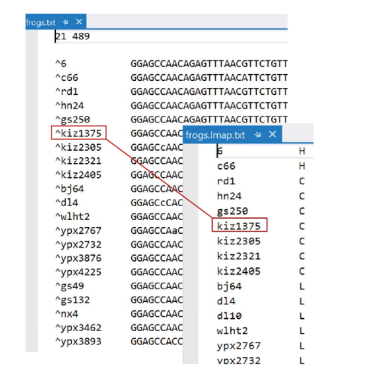
\includegraphics[scale=0.567890]{figures/fig-imap}
  \caption{An example Imap file showing the sequence ID in the Imap
    file corresponding to that in the sequence file. Note that the
    caret \^{} symbol is not allowed in the sequence ID of the Imap
    file but is required in the sequence label in the sequence data
    file.}
  \label{fig-imap}
\end{figure}

\section{Outgroups and Constraints File}
The \textbf{outgroups and constraints file} is optional and its name is
specified in the control file by setting variable
\texttt{constraintfile} to the name of the constraint file.
Topological constraints on species trees can only be specified for
analyses A01 (species tree inference with a fixed species
delimitation) and A11 (joint species tree inference and species
delimitation). See Chapter~\ref{analysismethods} for a detailed
description of the A01 and A11 methods of analysis.  Note that species
trees are always rooted in \textsc{bpp}, whether you use the clock or
relaxed clock. The control variable \texttt{constraintfile} in the
control file has the format
\begin{verbatim}
constraintfile = constraints.txt
\end{verbatim}
Inside the constraint file, three keywords are allowed:
\texttt{define}, \texttt{constraint}, and \texttt{outgroup}.  The
\texttt{define} keyword is used to assign a name or alias to a clade,
\texttt{constraint} defines a clade or subtree, and \texttt{outgroup}
means that species not on the list (the ingroup species) form a clade.
\begin{verbatim}
define g1 as (G,H);
# identical to constraint (D,E,F,(G,H));
constraint (D,E,F,g1);   
outgroup A,B,C;
constraint (A,B);
\end{verbatim}
Either the equal sign (=) or spaces can be used to separate the keyword from
the specified value. In the example above,
there are eight species in the dataset: A, B, C, D, E, F, G, and H.
Line 1 defines an alias \texttt{g1} for clade (G,H), which may be used
in subsequent \texttt{define} or \texttt{constraint} statements. Line
3 specifies A, B, C as the outgroups; this is interpreted to mean that
species not on the list, (that is, D, E, F, G and H) form a
clade. Since this information is already in line 2, line 3 has no
effect in this case.

The modifier keyword \texttt{NOT} (case-insensitive) can be used with
\texttt{define} to instead specify the complement of the species on the
list. Suppose in the data we have 10 species of ratites (flightless
birds), and two outgroup species, chicken and ostrich. You can specify
the constraint as follows:
\begin{verbatim}
define ratites as NOT (chicken, ostrich);
constraint = (chicken, (ostrich, ratites));
\end{verbatim}

Note that \textsc{bpp} interprets \texttt{outgroup} to mean that all
species not on the list form a clade. In theory the \texttt{outgroup}
keyword is unnecessary because you can always achieve the same thing
by using \texttt{define} (especially with the \texttt{NOT} option) and
\texttt{constraint}. However \texttt{outgroup} may be more convenient
or explicit in some situations. If there are four species
(A,B,C,D),
\begin{verbatim}
outgroup = B,C,D;
\end{verbatim}
achieves nothing since all the 15 rooted species trees are allowed,
whereas
\begin{verbatim}
outgroup = C,D;
\end{verbatim}
means (A,B) form a clade so that 3 rooted species trees are allowed.
Finally if multiple compatible constraints are specified, \textsc{bpp}
merges them into one so that
\begin{verbatim}
constraint (E,F,G,H);
constraint (F,G,H);
constraint (G,H);
\end{verbatim}
is equivalent to
\begin{verbatim}
constraint (E,(F,(G,H)));
\end{verbatim}
If any two constraints are in conflict, \textsc{bpp} will abort with
an error message. For example the following will cause an error.
\begin{verbatim}
constraint = (E,F,G,H);
constraint = (G,H);
constraint = (F,G);
\end{verbatim}

\section{Control File} \label{ctrlfile} The \textbf{control file} specifies
most aspects of a BPP analysis, including the names of input and
output files, choices of models, prior distributions on parameters,
etc.  The format is line oriented, with each line specifying the value
of a particular variable.  The default control file name is
\texttt{bpp.ctl}.  Lines beginning with \texttt{*} or \texttt{\#} are
comments and are ignored by the program.  Most often the order of the
lines is unimportant, but there are exceptions (as explained
below). Each non-commented line of the control file contains a
variable name and an assignment of one or more values to the
variable. The general syntax of a line in the control file is:
\begin{verbatim}
variable = value
\end{verbatim}
where \texttt{variable} is the name of a valid variable and
\texttt{value} is a list of one or more permissible values for the
variable.  Most variable assignments follow this format --- the
exceptions are described later.  BPP has complicated dependencies
among variables, both in terms of whether the variable needs to be
defined (or has a default value when undefined) and what
its permissible values are. Here we begin by defining
all the variable names, the syntax of their arguments and permissible
types (integers, floating point numbers, etc), and outline the
structure of dependencies among variables
(Table~\ref{variableTable}). Detailed definitions of the variables are
provided at the end of this section, ordered according to their
indexes in Table~\ref{variableTable}. If you are impatient to get started
using the program with worked examples, you might want to now skip
ahead to Section~\ref{examplecontrolfile} which explains the control
file variables in the context of a simple example dataset analysis.
You can later consult this section regarding particular
control file variables as the need arises.

Table~\ref{variableTable} lists all the variables that can be defined
in the BPP control file.  The first column lists an index used to
identify the variable in other columns of the table and to determine
the order in which the variables are defined in subsequent text. The
second column lists the variable name. The variable names are colored
to indicate the structure of their dependencies among variables as
follows:
\begin{itemize}
\item {\color{red} Red = variable always needs to be defined, has no
    default value, and does not depend on other variables.}
\item {\color{blue} Blue = variable always needs to be defined, has a
    default value if no value is provided in control file, and does
    not depend on other variables.}
\item {\color{yellow1} Yellow = whether variable needs to defined (and
    possibly also its permissible values) depends on the value of
    another variable.}
\item {\color{green1} Green = variable always needs to be defined and
    has no default value but its permissible values depend on the
    value of another variable.}
\end{itemize}
Column 3 lists the permissible types of each variable and the syntax
for specifying arguments in defining the variable. The variable types
are defined in Table~\ref{symbolTable}.
\begin{table}
  \begin{tabular}{@{}llr@{}}
    \toprule
    Symbol/Rule & Definition \\ \midrule
    b & Boolean (0,1) \\
    +d & Positive integer \\
    f & floating point number \\
    s & String (or character) \\
    t & Tree in Newick format \\
    x* & List of one or more elements of type x \\
    y [z] & z is a set of variables whose form is determined by y \\
    (w,z) & w and z are two different permissible types \\
    y [(w,z)] & whether w or z is the permissible type depends on value of y \\          
    \bottomrule
  \end{tabular}
  \caption{Symbols used to represent syntax and value types of
    variables in Table~\ref{variableTable}}
  \label{symbolTable}
\end{table}
Column~4 lists the condition (state of another variable) that either
determines whether the variable on that line exists (yellow1
variables) or determines its permissible values (blue and green
variables).  x[y] refers to value of argument y of the variable with
index x. Column~5 lists indexes of variables that either are
influenced by the variable (the notation ->[c,d] indicates that the
variable influences variables c and d) or variables that influence the
variable (the notation <-[a] indicates that variable a influences the
variable). If you are writing a control file from scratch, these
dependencies necessitate that you specify the red variables first,
followed by the blue (only needed if changing defaults) and then the
yellow/green.
\newpage
\begin{table}[h]
  \begin{center}
    {\small
    \begin{tabular}{@{}llllr@{}}
      \toprule
      Index & Variable & Values & Condition & Dependencies \\ \midrule
      1 & {\color{blue} seed} & (-d,+d) & True & None \\
      2 & {\color{blue} usedata} & b & True & None \\
      3 & {\color{red} outfile} & s & True& None \\
      4 & {\color{red} mcmcfile} & s & True & None \\
      5 & {\color{red} seqfile} & s & True & <-17 \\
      6 & {\color{red} finetune} & b [f*] & True & ->8 \\
      7 & {\color{red} print} & b b b b b & True & None \\
      8 & {\color{yellow1} burnin} & +d & True & <-6 \\
      9 & {\color{red} sampfreq} & +d & True & None \\
      10 & {\color{red} nsample} & +d & True & None \\
      11 & {\color{red} species\&tree} & +d s* +d* t & True & ->\{12,16,25\}  \\  
      12 & {\color{yellow1} Imapfile} & s & 11[1]>1 & <-11 \\
      13 & {\color{blue} speciesdelimitation} & b [b f*] & True & ->15 \\
      14 & {\color{blue} speciestree} & b & True & ->14 \\
      15 & {\color{yellow1} speciesmodelprior} & +d  & 13[1]=1 OR 14[1]=1 & <-\{13,14\} \\
      16 & {\color{green1} phase} & b* & 11[1] & <-11 \\
      17 & {\color{blue} nloci} & +d & True & ->5 <-31 \\
      18 & {\color{blue} model} & s & True & None \\
      19 & {\color{blue} Qrates} & b +f +f +f +f +f +f & 18=''7'' & <-18 \\
      20 & {\color{blue} basefreqs} & b +f +f +f +f & 18=''7'' & <-18 \\
      21 & {\color{blue} alphaprior} & f f +d & True & None \\
      22 & {\color{blue} cleandata} & b & True & None \\
      23 & {\color{red} thetaprior} & s [(f*, f f s)] & True & None \\
      24 & {\color{red} tauprior} & s f f & True & None \\
      25 & {\color{yellow1} phiprior} & f f & 11[4] & <-11 \\
      26 & {\color{blue} locusrate} & +d [(f f f s, s, )] & True & <-27 ->27 \\
      27 & {\color{blue} clock} & +d [f f f s s] & True & <-26 ->26 \\
      28 & {\color{blue} heredity} & +d [(f f, s)] & True & None \\
      29 & {\color{blue} checkpoint} & +d [(+d)] & True & None \\
      30 & {\color{blue} constraintfile} & s & True & None \\
      31 & {\color{yellow1} threads} & +d [ +d +d ] & True & ->17 \\
      \bottomrule
    \end{tabular}
    }
    \caption{List of BPP control variables. The column Variable
      contains the control file variable name, the column Values
      specifies using symbols the format of the values (symbols
      defined in Table~\ref{symbolTable}). The column Condition
      describes the conditions (if any) needed for the variable to be
      required. An entry of True in this column means that the
      variable is always required/defined although possibly not
      explicitly (there may be a default value). The column
      Dependencies lists the variables that either influence the
      variable (<-) or are influenced by the variable (->) with the
      variables denoted using their index from column Index.}
    \label{variableTable}
  \end{center}
\end{table}

\newpage
\subsection{BPP control file variables} \label{controlfilevariables}
\textbf{{\large 1}} \\
\noindent\rule{\textwidth}{0.8pt} \\
\textbf{{\Large \texttt{seed = (-d,+d)}}} \vspace{5pt}\\
\textbf{DESCRIPTION} \vspace{5pt}\\
Specifies the seed used for the random number generator.\vspace{5pt}\\
\textbf{VALUES} \vspace{5pt}\\
\textbf{\texttt{-d}}, use the wall clock (in Windows) or white noise (in Linux) to generate a seed (store seed in file \texttt{SeedUsed}).\vspace{5pt}\\
\textbf{\texttt{+d}}, use +d as the seed.\vspace{10pt}\\
\textbf{DEFAULT} \vspace{5pt}\\
\textbf{\texttt{-1}} \vspace{5pt}\\
\textbf{COMMENTS} \vspace{5pt}\\
Using the same positive integer seed will produce identical results in
different runs, which is useful for debugging, and using different
positive integers in different runs produces different results.  Using
$-d$, for example, $-1$, the computer's entropy generator is used as a source for the seed, and
different runs will produce different results. When evaluating MCMC convergence
by comparing results across different runs be sure to use -d. The positive integer
seed automatically generated when using option -d is stored in a file named SeedUsed and
can be used explicitly to replicate a result. It is recommended that
you run each analysis at least twice using different seeds to confirm that the results are stable across runs. \vspace{5pt}\\
\textbf{EXAMPLES} \vspace{5pt}\\
\textbf{\texttt{seed = -1}}\vspace{5pt}\\
\textbf{\texttt{seed = 278}}\vspace{10pt}\\
\textbf{{\large 2}} \\
\noindent\rule{\textwidth}{0.8pt} \\
\textbf{{\Large \texttt{usedata = b}}} \vspace{5pt}\\
\textbf{DESCRIPTION} \vspace{5pt}\\
Specifies whether data (likelihood+priors) are used in calculating probabilities during MCMC or only priors.\vspace{5pt}\\
\textbf{VALUES} \vspace{5pt}\\
\textbf{\texttt{0}}, use only the priors to calculate probabilities (likelihood constant).\vspace{5pt}\\
\textbf{\texttt{1}}, use likelihood and prior probabilities. \vspace{5pt}\\
\textbf{DEFAULT}\vspace{5pt}\\
\textbf{\texttt{1}} \vspace{5pt}\\
\textbf{COMMENTS} \vspace{5pt}\\
The \textbf{\texttt{0}} option can be used for debugging, or examining priors. When using option \textbf{\texttt{0}} a MCMC run produces samples from the prior for each variable. \vspace{5pt}\\
\textbf{EXAMPLES} \vspace{5pt}\\
\textbf{\texttt{usedata = 0}} \vspace{5pt}\\
\textbf{\texttt{usedata = 1}} \vspace{10pt}\\

\noindent\textbf{{\large 3}} \\
\noindent\rule{\textwidth}{0.8pt} \\
\textbf{{\Large \texttt{outfile = s}}} \vspace{5pt}\\
\textbf{DESCRIPTION} \vspace{5pt}\\
Sets the path/name of the output file to be the string \textbf{\texttt{s}} \vspace{5pt}\\
\textbf{VALUES} \vspace{5pt}\\
\textbf{\texttt{s}}, a string of characters specifying the directory path and name of file that will receive the program output. \vspace{5pt}\\
\textbf{EXAMPLES} \vspace{5pt}\\
\textbf{\texttt{outfile = /home/mickey/mouse\_out.txt}} \vspace{10pt}\\
\textbf{{\large 4}} \\
\noindent\rule{\textwidth}{0.8pt} \\
\textbf{{\Large \texttt{mcmcfile = s}}} \vspace{5pt} \\
\textbf{DESCRIPTION} \vspace{5pt}\\
Sets the name of the file receiving MCMC output to be the string \textbf{\texttt{s}} \vspace{5pt}\\
\textbf{VALUES} \vspace{5pt}\\
\textbf{\texttt{s}}, a string of characters specifying the directory path and name of file that will receive the MCMC output. \vspace{5pt}\\
\textbf{EXAMPLES} \vspace{5pt}\\
\textbf{\texttt{mcmcfile = /home/mickey/mouse\_mcmc.txt}} \vspace{5pt}\\
\textbf{\texttt{mcmcfile = mcmc.txt}} \vspace{10pt}\\
\textbf{{\large 5}} \\
\noindent\rule{\textwidth}{0.8pt} \\
\textbf{{\Large \texttt{seqfile = s}}} \vspace{5pt} \\
\textbf{DESCRIPTION} \vspace{5pt}\\
Sets the name of the file containing the sequence data to be the string \textbf{\texttt{s}} \vspace{5pt}\\
\textbf{VALUES} \vspace{5pt}\\
\textbf{\texttt{s}}, a string of characters specifying the directory path and name of file that contains the sequence data \vspace{5pt}\\
\textbf{EXAMPLES} \vspace{5pt}\\
\textbf{\texttt{seqfile = /home/mickey/mouse\_seq.txt}} \vspace{5pt}\\
\textbf{\texttt{seqfile = sequences.txt}} \vspace{10pt}\\

\textbf{{\large 6}} \\
\noindent\rule{\textwidth}{0.8pt} \\
\textbf{{\Large \texttt{finetune = b: [f*]}}} \vspace{5pt}\\
\textbf{DESCRIPTION} \vspace{5pt}\\
Determines whether step lengths in MCMC proposals are automatically optimized or manually set to fixed values as well as setting either the fixed step lengths (manual) or the starting step lengths (optimized). There are up to
15 proposals with step lengths that can be adjusted. Not all proposals are defined for any given choice of model and analysis,
however 15 values should always be specified when using manual as the order is fixed, step lengths specified for unused proposals will be ignored by the program. The sizes of proposal steps for each parameter are provided (from left to right) in the same order as listed (from top to bottom in table.
The proposals are as follows:
\begin{table}[h]
\begin{tabular}{ll}
\hline
Abbreviation & Parameter Proposal Description \\ \hline
Gage & Node age on gene tree \\
Gspr & Subtree pruning and regrafting move \\
thet & Theta \\
tau &  Tau \\
mix &  Mixing step (jointly changing mu, tau and gene tree node ages\\
lrht & empty \\
phi &  Introgression probability\\
pi &  Stationary frequencies of substitution model\\
qmat &  Q matrix elements of substitution model \\
alfa &  Alpha parameter of gamma model for rate variation among sites \\
mubr &  empty \\
nubr &  empty \\
mu\_i &  empty \\
nu\_i &  empty \\
brte &  empty \\ \hline
\end{tabular}
\end{table}
\vspace{5pt}\\
\textbf{VALUES} \vspace{5pt}\\
\textbf{\texttt{0: Gage Gspr thet tau mix lrht phi pi qmat alfa mubr nubr mu\_i nu\_i brte}}\\
Use fixed step lengths in MCMC proposals as specified, where Gage is the specified step length for proposal Gage, and so on. \vspace{5pt}\\
\textbf{\texttt{1: Gage Gspr thet tau mix lrht phi pi qmat alfa mubr nubr mu\_i nu\_i brte}}\\
Automatically optimize step lengths in MCMC proposals using specified initial step lengths. \vspace{5pt}\\
\textbf{DEFAULT} \vspace{5pt}\\
\textbf{\texttt{0}} \\
Manually fixes all step lengths to be $0.1$.\\
\textbf{\texttt{1}} \\
Fixes all initial proposal step lengths to $0.1$ prior to optimization.\\ 
\textbf{DEPENDENCIES} \vspace{5pt}\\
If \textbf{\texttt{b}} is set to 1 (automatic optimization) then \textbf{\texttt{burnin}} has to be >200. \vspace{5pt}\\
\textbf{COMMENTS} \vspace{5pt}\\
The first value, before the colon, is a switch, with 0 meaning no
automatic adjustments by the program and 1 meaning automatic
adjustments by the program.  Following the colon are the step lengths
for the proposals used in the program.  and then the step lengths
specified here will be the initial step lengths, and the program will
try to adjust them using the information collected during the burnin
step.  This option appears to work fine.  Some notes about manually
adjusting those finetune step lengths are provided below in section
3.2. \vspace{5pt}\\
\textbf{EXAMPLES} \vspace{5pt}\\
\textbf{\texttt{finetune = 0: .01 .02 .03 .04 .05 .01 .01 .01 .01 .01 .01 .01 .01 .01 .01}} \vspace{5pt}\\
\textbf{\texttt{finetune = 1}}\vspace{10pt}\\
\textbf{{\large 7}} \\
\noindent\rule{\textwidth}{0.8pt} \\
\textbf{{\Large \texttt{print = b b b b b}}} \vspace{5pt}\\
\textbf{DESCRIPTION} \vspace{5pt}\\
Specifies what information is saved to the output files during the
MCMC.
\vspace{5pt}\\
\textbf{VALUES} \vspace{5pt}\\
There are 5 boolean (0,1) variables that specify whether particular
variables are saved to file (1) or not saved (0). From left to right:
variable 1 specifies MCMC samples; variable 2 specifies locus-specific
rate parameters (rate $\mu_i$, variance parameter $\nu_i$ and
species-tree branch rates for locus $r_{ij}$); variable 3 specifies
locus-specific heredity scalars if those are estimated from the data;
variable 4 specifies locus-specific gene trees; and variable 5
specifies locus-specific substitution-rate parameters (qmat for the
$Q$ matrix, freqs for base
frequencies, and alpha for gamma rates for sites).  \vspace{5pt}\\
\textbf{EXAMPLES} \vspace{5pt}\\
\textbf{\texttt{print = 0 1 1 1 0}} \vspace{5pt}\\
\textbf{\texttt{print = 1 1 1 1 1}} \vspace{10pt}\\
\textbf{{\large 8}} \\
\noindent\rule{\textwidth}{0.8pt} \\
\textbf{{\Large \texttt{burnin = +d}}} \vspace{5pt}\\
\textbf{DESCRIPTION} \vspace{5pt}\\
Specifies the number of burn-in iterations that are executed in the
MCMC run before sampling begins.
\vspace{5pt}\\
\textbf{VALUES} \vspace{5pt}\\
\textbf{\texttt{+d}}, a positive integer specifying the number of burn-in iterations. \vspace{5pt}\\
\textbf{DEPENDENCIES} \vspace{5pt}\\
If \textbf{\texttt{finetune = 1}} (automatic optimization) then \textbf{\texttt{burnin}} has to be >200. \vspace{5pt}\\
\textbf{COMMENTS} \vspace{5pt}\\
The total number of MCMC iterations is \textbf{\texttt{burnin}} + \textbf{\texttt{nsample $\times$ sampfreq}}. \vspace{5pt}\\
\textbf{EXAMPLES} \vspace{5pt}\\
\textbf{\texttt{burnin = 100}} \vspace{5pt}\\
\textbf{\texttt{burnin = 10000}}\vspace{10pt}\\
\textbf{{\large 9}} \\
\noindent\rule{\textwidth}{0.8pt} \\
\textbf{{\Large \texttt{sampfreq = +d}}} \vspace{5pt}\\
\textbf{DESCRIPTION} \vspace{5pt}\\
Specifies the interval at which samples from the MCMC are to be written to the output file specified by \textbf{\texttt{mcmcfile}}. \vspace{5pt}\\
\textbf{VALUES} \vspace{5pt}\\
\textbf{\texttt{+d}}, a positive integer specifying the interval between samples from the MCMC. \vspace{5pt}\\
\textbf{COMMENTS} \vspace{5pt}\\
The total number of MCMC iterations is \textbf{\texttt{burnin}} + \textbf{\texttt{nsample $\times$ sampfreq}}. \vspace{5pt}\\
\textbf{EXAMPLES} \vspace{5pt}\\
\textbf{\texttt{sampfreq = 2}} \vspace{5pt}\\
\textbf{\texttt{sampfreq = 10}}\vspace{10pt}\\
\textbf{{\large 10}} \\
\noindent\rule{\textwidth}{0.8pt} \\
\textbf{{\Large \texttt{nsample = +d}}} \vspace{5pt}\\
\textbf{DESCRIPTION} \vspace{5pt}\\
Specifies the number of samples from the MCMC that are to be written to the output file specified by \textbf{\texttt{mcmcfile}}. \vspace{5pt}\\
\textbf{VALUES} \vspace{5pt}\\
\textbf{\texttt{+d}}, a positive integer specifying the number of MCMC samples. \vspace{5pt}\\
\textbf{COMMENTS} \vspace{5pt}\\
The total number of MCMC iterations is \textbf{\texttt{burnin}} + \textbf{\texttt{nsample $\times$ sampfreq}}. \vspace{5pt}\\
\textbf{EXAMPLES} \vspace{5pt}\\
\textbf{\texttt{nsample = 5000}} \vspace{5pt}\\
\textbf{\texttt{nsample = 25499}}\vspace{10pt}\\
\textbf{{\large 11}} \\
\noindent\rule{\textwidth}{0.8pt} \\
\textbf{{\Large \texttt{species\&tree = +d s*}}} \vspace{2pt}\\
\hspace*{9.2pc} \textbf{{\Large \texttt{+d*}}} \vspace{2pt}\\
\hspace*{9.2pc} \textbf{{\Large \texttt{t}}} \vspace{5pt}\\
\textbf{DESCRIPTION} \vspace{5pt}\\
Specifies the number of species, the species names, the maximum number of sequences (at any locus) for each species, and the species tree in Newick format (or species graph in extended Newick format in models with introgression).\vspace{5pt}\\
\textbf{VALUES} \vspace{5pt}\\
\textbf{\texttt{+d}}, a positive integer specifying the total number of species. \textbf{\texttt{s*}}, a list of \textbf{\texttt{+d}} strings specifying the name of each species. \textbf{\texttt{+d*}}, a list of \textbf{\texttt{+d}} positive integers specifying the maximum number of sequences (at any locus) for each species. \textbf{\texttt{t}}, a tree (or graph) in Newick format (or Newick extended format) specifying the relationships among species (and possibly introgression events). \vspace{5pt}\\
\textbf{DEPENDENCIES} \vspace{5pt}\\
The variable \textbf{\texttt{Imapfile}} must be specified only when
the number of species $\textbf{\texttt{+d}} > 1$. The length of the
boolean array specified for variable \textbf{\texttt{phase}} is equal
to the number of species \textbf{\texttt{+d}}. The variable
\textbf{\texttt{phiprior}} must be specified only if
\textbf{\texttt{t}} is an introgression graph.
\vspace{5pt}\\
\textbf{COMMENTS} \vspace{5pt}\\
See the subsection \emph{Notation for trees and introgression graphs}
for details on the format of \textbf{\texttt{t}}. The role of
\textbf{\texttt{t}} in the MCMC analysis depends on the value of the
\textbf{\texttt{speciestree}} variable. If
\textbf{\texttt{speciestree=1}} the variable \textbf{\texttt{t}}
specifies the starting tree for the MCMC analysis, otherwise if
\textbf{\texttt{speciestree=0}} it is the fixed tree used for
estimating parameters or the fixed guide tree for species
delimitation.
\vspace{5pt}\\
\textbf{EXAMPLES} \vspace{5pt}\\
\textbf{\texttt{species\&tree = 4  H  C  G  O}} \vspace{2pt}\\
\hspace*{7.2pc}  \textbf{\texttt{1  1  1  1}} \vspace{2pt}\\
\hspace*{7.2pc}  \textbf{\texttt{(((H, C), G), O);}} \vspace{10pt}\\
\textbf{{\large 12}} \\
\noindent\rule{\textwidth}{0.8pt} \\
\textbf{{\Large \texttt{Imapfile = s}}} \vspace{5pt}\\
\textbf{DESCRIPTION} \vspace{5pt}\\
Sets the path/name of the Imap file to be the string \textbf{\texttt{s}}. \vspace{5pt}\\
\textbf{VALUES} \vspace{5pt}\\
\textbf{\texttt{s}}, a string of characters specifying the directory path and name of a file that contains the species/sequence map information. \vspace{5pt}\\
\textbf{DEPENDENCIES} \vspace{5pt}\\
The variable \textbf{\texttt{Imapfile}} must be specified only when the number of species defined by the \textbf{\texttt{species\&tree}} variable $\textbf{\texttt{+d}} > 1$. \vspace{5pt}\\
\textbf{COMMENTS} \vspace{5pt}\\
See section~\ref{imapfile} for a complete description of the Imap file format. \vspace{5pt} \\
\textbf{EXAMPLES} \vspace{5pt}\\
\textbf{\texttt{Imapfile = /home/foo/bar\_Imap.txt}} \vspace{5pt}\\
\textbf{\texttt{Imapfile = Imap.txt}} \vspace{10pt}\\
\textbf{{\large 13}} \\
\noindent\rule{\textwidth}{0.8pt} \\
\textbf{{\Large \texttt{speciesdelimitation = b [b f*]}}} \vspace{5pt}\\
\textbf{DESCRIPTION} \vspace{5pt}\\
Specifies whether species delimitation is performed and if so
specifies the parameters of the species delimitation rjMCMC proposal
algorithm. \vspace{5pt}\\
\textbf{VALUES} \vspace{5pt}\\
\textbf{\texttt{0}}, specifies no species delimitation. \vspace{5pt}\\
\textbf{\texttt{1 0 $\epsilon$}}, specifies species delimitation with rjMCMC algorithm 0, with parameter $\epsilon$ as specified in equations 3 and 4 of \cite{Yang2010}.  Reasonable values for $\epsilon$ are 1, 2, 5, etc. \vspace{5pt}\\
\textbf{\texttt{1 1 $\alpha$ m}}, specifies rjMCMC algorithm 1, with
parameters $ \alpha$ and $m$ as specified in equations 6 and 7 of
\cite{Yang2010}. Reasonable values are $\alpha = 1, 1.5, 2$, etc. and $m = 0.5, 1, 2$. \vspace{5pt}\\
\textbf{DEFAULT} \vspace{5pt}\\
\textbf{\texttt{0}} \vspace{5pt}\\
\textbf{DEPENDENCIES} \vspace{5pt}\\
If \textbf{\texttt{speciesdelimitation = 1}} then \textbf{\texttt{speciesmodelprior}} must be defined. \vspace{5pt}\\
\textbf{EXAMPLES} \vspace{5pt}\\
\textbf{\texttt{speciesdelimitation = 1 0 2}} \vspace{5pt}\\
\textbf{\texttt{speciesdelimitation = 1 1 2 1}}\vspace{10pt}\\
\textbf{{\large 14}} \\
\noindent\rule{\textwidth}{0.8pt} \\
\textbf{{\Large \texttt{speciestree = b}}} \vspace{5pt}\\
\textbf{DESCRIPTION} \vspace{5pt}\\
Specifies whether the species tree is estimated or fixed in the MCMC
analysis.
\vspace{5pt}\\
\textbf{VALUES} \vspace{5pt}\\
\textbf{\texttt{0}}, specifies that species tree is fixed.  \vspace{5pt}\\
\textbf{\texttt{1}}, specifies that species tree is estimated. \vspace{5pt}\\
\textbf{\texttt{}} \vspace{5pt}\\
\textbf{DEFAULT} \vspace{5pt}\\
\textbf{\texttt{0}} \vspace{5pt}\\
\textbf{DEPENDENCIES} \vspace{5pt}\\
If \textbf{\texttt{speciestree = 1}} then \textbf{\texttt{speciesmodelprior}} must be defined. \vspace{5pt}\\
\vspace{5pt}\\
\textbf{COMMENTS} \vspace{5pt}\\
This option invokes the nearest-neighbor interchange (NNI) or
subtree-pruning-regrafting (SPR) algorithm to propose changes to the
species tree topology during the MCMC run.
\vspace{5pt}\\
\textbf{EXAMPLES} \vspace{5pt}\\
\textbf{\texttt{speciestree = 1}} \vspace{5pt}\\
\textbf{\texttt{speciestree = 0}}\vspace{10pt}\\
\textbf{{\large 15}} \\
\noindent\rule{\textwidth}{0.8pt} \\
\textbf{{\Large \texttt{speciesmodelprior}}} \vspace{5pt}\\
\textbf{DESCRIPTION} \vspace{5pt}\\
Specifies the prior distribution for rooted species trees and species delimitations. \vspace{5pt}\\
\textbf{VALUES} \vspace{5pt}\\
\textbf{\texttt{0}}, specifies equal probabilities for the labeled histories (rooted trees with the internal nodes ordered by age). \vspace{5pt}\\
\textbf{\texttt{1}}, specifies equal probabilities for the rooted species trees. \vspace{5pt}\\
\textbf{\texttt{2}}, specifies equal probabilities for the numbers of species ($1/s$ each for $1,2,\ldots,s$ species given $s$ populations) and divides the probability for any specific number of species among the compatible models (of species delimitation and species phylogeny) in proportion to the number of labeled histories. \vspace{5pt}\\
\textbf{\texttt{3}}, specifies equal probabilities for the numbers of species ($1/s$ each for $1,2,\ldots,s$ species given $s$ populations) and divides the probability for any specific number of species among the compatible models (of species delimitation and species phylogeny) uniformly. \vspace{5pt}\\
\textbf{DEPENDENCIES} \vspace{5pt}\\
The variable \textbf{\texttt{speciesmodelprior}} must be defined if either (or both) \textbf{\texttt{speciestree = 1}} or \textbf{\texttt{speciesdelimitation = 1}}. If \textbf{\texttt{speciestree = 1}} and \textbf{\texttt{speciesdelimitation = 0}} then only options \textbf{\texttt{speciesmodelprior = 0}} or \textbf{\texttt{speciesmodelprior = 1}} may be used.\vspace{5pt}\\
\textbf{COMMENTS} \vspace{5pt}\\
The priors specified by options 2 and 3 are discussed by
\cite{Yang2014a} and implemented by \cite{Yang2015}. The prior
specified by option 3 may be
suitable when there are many populations. \vspace{5pt}\\
\textbf{EXAMPLES} \vspace{5pt}\\
\textbf{\texttt{speciesmodelprior = 0}} \vspace{5pt}\\
\textbf{\texttt{speciesmodelprior = 3}}\vspace{10pt}\\
\textbf{{\large 16}} \\
\noindent\rule{\textwidth}{0.8pt} \\
\textbf{{\Large \texttt{phase = b*}}} \vspace{5pt}\\
\textbf{DESCRIPTION} \vspace{5pt}\\
Specifies whether the sequence data for each species is phased.
\vspace{5pt}\\
\textbf{VALUES} \vspace{5pt}\\
\textbf{\texttt{1}}, in position $i$ of the list indicates that data is unphased for species $i$ in the list of species in variable \textbf{\texttt{species\&tree}}, otherwise \textbf{\texttt{0}} indicates it is phased. \vspace{5pt}\\
\textbf{DEFAULT} \vspace{5pt}\\
\textbf{\texttt{0}} \vspace{5pt}\\
\textbf{DEPENDENCIES} \vspace{5pt}\\
The number of boolean (0,1) variables in the list must equal the number of species \textbf{\texttt{d+}} specified in the \textbf{\texttt{species\&tree}} variable. \vspace{5pt}\\
\textbf{COMMENTS} \vspace{5pt}\\
If at position $i$ the \textbf{\texttt{phase}} variable is 1, each
sequence from species $i$ is treated as an unphased diploid sequence,
with heterozygous sites represented using the ambiguity characters
\texttt{YRMKSW}.  The missing data tokens \texttt{N-?} are allowed and
are all treated as ?, but other ambiguity characters (\texttt{HBVD})
are not allowed.

For phasing, each sequence is expanded/resolved into two sequences,
and the program averages over possible phase resolutions according to
the approach of \citet{Gronau2011}.  For example, a sequence
\texttt{R...Y} with two heterozygous sites, \texttt{R} (meaning
\texttt{A/G}) and \texttt{Y} (meaning \texttt{C/T}), has two possible
phase resolutions:
\begin{enumerate}
\item \texttt{A...T} and \texttt{G...C}
\item \texttt{A...C} and \texttt{G...T}
\end{enumerate}
A sequence with no heterozygous sites will be phased/resolved into two
identical sequences.  The MSC model effectively averages over
different phase resolutions of the heterozygous sites in performing
the likelihood calculation.  The option may increase memory usage and
CPU time considerably if many sequences exist with many heterozygote
sites at a locus.  If the \textbf{\texttt{phase}} variable for a
species is 0, all sequences from that species are treated as resolved
haplotype sequences, and ambiguities are interpreted in the usual
way. For example, an ambiguity code \texttt{Y} at a position is
interpreted to mean that one sequence exists with an uncertain
nucleotide at that position that is either a T or a C.  The program
does not allow some sequences from a species to be phased and other
sequences from that same species to be unphased.  \vspace{5pt}\\
\textbf{EXAMPLES} \vspace{5pt}\\
\textbf{\texttt{phase = 0 0 0 0 1}} \vspace{5pt}\\
\textbf{\texttt{phase = 1 1 1 1 1}}\vspace{10pt}\\
\textbf{{\large 17}} \\
\noindent\rule{\textwidth}{0.8pt} \\
\textbf{{\Large \texttt{nloci = +d}}} \vspace{5pt}\\
\textbf{DESCRIPTION} \vspace{5pt}\\
Specifies the number of loci present in the sequence data file
specified by variable \textbf{\texttt{seqfile}}
that will be analysed. \vspace{5pt}\\
\textbf{VALUES} \vspace{5pt}\\
\textbf{\texttt{+d}}, a positive integer specifying the number of loci to be analyzed. \vspace{5pt}\\
\textbf{DEFAULT} \vspace{5pt}\\
If \textbf{\texttt{nloci}} is not specified, all the loci present in the sequence file specified by \textbf{\texttt{seqfile}} will be analysed. \vspace{5pt}\\
\textbf{DEPENDENCIES} \vspace{5pt}\\
\textbf{\texttt{nloci}} must be less than or equal to the number of loci available in the sequence file specified by \textbf{\texttt{seqfile}}.  \vspace{5pt}\\
\textbf{COMMENTS} \vspace{5pt}\\
If \textbf{\texttt{nloci}} is less than the number of loci present in
the file specified by \textbf{\texttt{seqfile}} only the first
\textbf{\texttt{nloci}} present
in that file wil be analysed. \vspace{5pt}\\
\textbf{EXAMPLES} \vspace{5pt}\\
\textbf{\texttt{nloci = 1}} \vspace{5pt}\\
\textbf{\texttt{nloci = 2000}}\vspace{10pt}\\
\textbf{{\large 18}} \\
\noindent\rule{\textwidth}{0.8pt} \\
\textbf{{\Large \texttt{model = s [s]}}} \vspace{5pt}\\
\textbf{DESCRIPTION} \vspace{5pt}\\
Specifies the DNA substitution model (or amino acid substitution model) that will be used. For DNA sequences
the simplest (default) model that can be chosen is the Jukes-Cantor (JC69) model and the most complex is the
General Time-Reversible (GTR) model. A range of models of intermediate complexity are also available. For
amino acid sequences, most of the commonly used amino acid substitution matrix models are available. If a model other than \texttt{Custom}
is specified it will apply to all loci. If \texttt{Custom filename} is specified, an additional file \texttt{filename} must be provided that contains
one or more lines with the format:
\begin{verbatim}
loci_indices data_type model
\end{verbatim}
where \texttt{loci\_indices} is an index or range of indexes for loci (indexed according to their order of occurrence in the sequence data file),
\texttt{data\_type} is either \texttt{DNA} or \texttt{AA}, and model specifies the substitution model variable for the indexed loci as described above.
For example, the entry
\begin{verbatim}
1-10 DNA JC69
11 AA DAYHOFF
\end{verbatim}
specifies that loci 1 to 10 comprise DNA sequences that will have the \texttt{JC69} model applied to them, while locus 11 is an amino acid sequence
that will have the \texttt{DAYHOFF} model applied to it.
\vspace{5pt}\\
\textbf{VALUES} \vspace{5pt}\\
For DNA sequences: \textbf{\texttt{JC69}}, \textbf{\texttt{K80}}, \textbf{\texttt{F81}}, \textbf{\texttt{HKY}}, \textbf{\texttt{T92}},
\textbf{\texttt{TN93}}, \textbf{\texttt{F84}}, \textbf{\texttt{GTR}}. \vspace{5pt}\\
For amino acid sequences: \textbf{\texttt{DAYHOFF}}, \textbf{\texttt{LG}}, \textbf{\texttt{DCMUT}}, \textbf{\texttt{JTT}}, \textbf{\texttt{MTREV}},
\textbf{\texttt{WAG}}, \textbf{\texttt{RTREV}}, \textbf{\texttt{CPREV}}, \textbf{\texttt{VT}}, \textbf{\texttt{BLOSUM62}}, \textbf{\texttt{MTMAM}},
\textbf{\texttt{MTART}}, \textbf{\texttt{MTZOA}}, \textbf{\texttt{PMB}}, \textbf{\texttt{HIVB}}, \textbf{\texttt{HIVW}}, \textbf{\texttt{JTTDCMUT}},
\textbf{\texttt{FLU}}, and \textbf{\texttt{STMTREV}}. \vspace{5pt}\\
Among-locus model variation: \textbf{\texttt{Custom filename}}. \vspace{5pt}\\
\textbf{DEFAULT} \vspace{5pt}\\
\textbf{\texttt{JC69}} \vspace{5pt}\\
\textbf{DEPENDENCIES} \vspace{5pt}\\
If \textbf{\texttt{model = GTR}} the variables \textbf{\texttt{Qrates}}
and \textbf{\texttt{basefreqs}} can be optionally defined which provide priors on the rate matrix and base frequencies, respectively (default priors will be used otherwise).
\vspace{5pt}\\
\textbf{EXAMPLES} \vspace{5pt}\\
\textbf{\texttt{model = GTR}} \vspace{5pt}\\
\textbf{\texttt{model = CPREV}}\vspace{5pt}\\
\textbf{\texttt{model = Custom models.txt}}\vspace{10pt}\\
\textbf{{\large 19}} \\
\noindent\rule{\textwidth}{0.8pt} \\
\textbf{{\Large \texttt{Qrates = b +f +f +f +f +f +f}}} \vspace{5pt}\\
\textbf{DESCRIPTION} \vspace{5pt}\\
Specifies whether the exchangeability parameters in the GTR model are
fixed or variable and
either their fixed values or prior relative mean values. \vspace{5pt}\\
\textbf{VALUES} \vspace{5pt}\\
\textbf{\texttt{b}}, specifies either fixed (1) or variable (0) exchangeability parameters in the GTR model. \vspace{5pt}\\
\textbf{\texttt{+f +f +f +f +f +f}}, specify the exchangeability
parameters in the order $a, b, c, d, e, f$ for TC, TA, TG, CA, CG, and
AG, as described in \citealt{Yang1994a}.
\vspace{5pt}\\
\textbf{DEFAULT} \vspace{5pt}\\
\textbf{\texttt{0 1 2 1 1 2 1}} \vspace{5pt}\\
\textbf{DEPENDENCIES} \vspace{5pt}\\
The variable \textbf{\texttt{Qrates}} is defined only if
\textbf{\texttt{model = GTR}}.
\vspace{5pt}\\
\textbf{COMMENTS} \vspace{5pt}\\
Two example cases are discussed here with either fixed, or variable
rates.  The following specifies fixed rates:
\begin{verbatim}
Qrates = 1  2 1 1 1 1 2
\end{verbatim}
This specifies fixed rates at $a = 2, b = c = d = e = 1$ and $f = 2$,
so that the transition rate is twice as high as the transversion rate,
and the model corresponds to K80 or HKY.  Note that only the relative
rates matter, because the rate matrix ($Q$) is scaled so that the
average rate (over the base frequencies) is 1 and branch lengths are
measured in the expected number of mutations/substitutions per site.
Nevertheless the program expects six rate parameters.
\begin{verbatim}
Qrates = 0  10 5 5 5 5 10 
\end{verbatim}
This specifies variable rates with a prior on $a, b, c, d, e$ that is
a Dirichlet distribution for every locus.  The above specifies Dir(10,
5, 5, 5, 5, 10), with parameters
$\alpha_a = 10, \alpha_b = \alpha_c = \alpha_d = \alpha_e = 10$, and
$\alpha_f = 10$.  The rates generated from the Dirichlet sum to 1, and
they are rescaled.  Note that larger values for those parameters mean
less variance, while the mean for $a$, say, is given by
$\alpha_a/\alpha$ with
$\alpha = \alpha_a + \alpha_b + \alpha_c + \alpha_d + \alpha_e +
\alpha_f$.
This specifies an average transition/transversion rate ratio of 2 (if base frequencies are all fixed at $\frac{1}{4}$). \vspace{5pt}\\
\textbf{EXAMPLES} \vspace{5pt}\\
\textbf{\texttt{Qrates = 1  2 1 1 1 1 2}} \vspace{5pt}\\
\textbf{\texttt{Qrates = 0  1 1 1 1 1 1}}\vspace{10pt}\\
\textbf{{\large 20}} \\
\noindent\rule{\textwidth}{0.8pt} \\
\textbf{{\Large \texttt{basefreqs = b +f +f +f +f}}} \vspace{5pt}\\
\textbf{DESCRIPTION} \vspace{5pt}\\
Specifies whether the base frequency parameters are fixed or variable
and either their fixed values or prior relative mean values. \vspace{5pt}\\
\textbf{VALUES} \vspace{5pt}\\
\textbf{\texttt{b}}, specifies either fixed (1) or variable (0) base frequency parameters in the GTR model. \vspace{5pt}\\
\textbf{\texttt{+f +f +f +f}}, specify the base frequency parameters in the order TCAG. \vspace{5pt}\\
\textbf{DEFAULT} \vspace{5pt}\\
\textbf{\texttt{0 1 1 1 1}} \vspace{5pt}\\
\textbf{DEPENDENCIES} \vspace{5pt}\\
The variable \textbf{\texttt{basefreqs}} is defined only if
\textbf{\texttt{model = GTR}}.
\vspace{5pt}\\
\textbf{COMMENTS} \vspace{5pt}\\
The parameters $\pi_T, \pi_C, \pi_A, \pi_G$ can be either fixed or
variable with a prior specified by the Dirichlet distribution
with $\alpha$ parameters specifying the relative mean frequencies. \vspace{5pt}\\
\textbf{EXAMPLES} \vspace{5pt}\\
\textbf{\texttt{basefreqs = 1 0.15 0.35 0.15 0.35 }} \vspace{5pt}\\
\textbf{\texttt{basefreqs = 0  10  10 10  10 }}\vspace{10pt}\\
\textbf{{\large 21}} \\
\noindent\rule{\textwidth}{0.8pt} \\
\textbf{{\Large \texttt{alphaprior = f f +d }}} \vspace{5pt}\\
\textbf{DESCRIPTION} \vspace{5pt}\\
Specifies the prior probability density for the shape parameter
controlling the pattern of among-site rate variation.
\vspace{5pt}\\
\textbf{VALUES} \vspace{5pt}\\
\textbf{\texttt{f f +d}}, specify the $\alpha_p$ and $\beta_p$
parameters of the prior on the Gamma shape parameter and the number of
rate
categories ncatG, respectively. \vspace{5pt}\\
\textbf{DEFAULT} \vspace{5pt}\\
$\alpha=\infty$ (no rate variation among sites) \vspace{5pt}\\
\textbf{COMMENTS} \vspace{5pt}\\
Among-site rate variation is assumed to follow a Gamma distribution
with a mean of 1 and shape parameter $\alpha$. The variance of rates
among sites is $1/\alpha$ and therefore a smaller $\alpha$ specifies
more rate variation.  A discrete distribution is used to efficiently
approximate the Gamma distribution and ncatG is the number of rate
categories used in the approximation -- more rate categories provide a
better approximation but incur greater computational expense. A value
for ncatG of 4 is recommended. The prior on $\alpha$ is also a Gamma
distribution with parameters $\alpha_p$ and $\beta_p$.  The variance
and mean of the prior on $\alpha$ are:
\begin{eqnarray}
  \textrm{Mean}(\alpha) & = & \frac{\alpha_p}{\beta_p}, \nonumber \\
  \textrm{Var}(\alpha) & = & \frac{\alpha_p}{\beta_p^2} \nonumber
\end{eqnarray}
\textbf{EXAMPLES} \vspace{5pt}\\
\textbf{\texttt{alphaprior = 1 1 4}} \vspace{10pt}\\
\textbf{{\large 22}} \\
\noindent\rule{\textwidth}{0.8pt} \\
\textbf{{\Large \texttt{cleandata = b}}} \vspace{5pt}\\
\textbf{DESCRIPTION} \vspace{5pt}\\
Specifies whether columns in the alignment which have gaps or
ambiguity characters will be removed prior to analysis, or will
instead be retained for use in the likelihood calculation.
\vspace{5pt}\\
\textbf{VALUES} \vspace{5pt}\\
\textbf{\texttt{0}}, specifies that columns in the alignment which
have gaps or ambiguity
characters will be treated as missing data and used in the likelihood calculation. \vspace{5pt}\\
\textbf{\texttt{1}}, specifies the removal of columns in the alignment
which have gaps or ambiguity
characters. \vspace{5pt}\\
\textbf{DEFAULT} \vspace{5pt}\\
\textbf{\texttt{0}} \vspace{5pt}\\
\textbf{EXAMPLES} \vspace{5pt}\\
\textbf{\texttt{cleandata = 1}} \vspace{5pt}\\
\textbf{\texttt{cleandata = 0}}\vspace{10pt}\\
\textbf{{\large 23}} \\
\noindent\rule{\textwidth}{0.8pt} \\
\textbf{{\Large \texttt{thetaprior =  s [(f*, f f s)] }}} \vspace{5pt}\\
\textbf{DESCRIPTION} \vspace{5pt}\\
Specifies the distribution model and parameters of the prior
distribution on the contemporary and ancestral population parameters
$\theta$ and whether the MCMC integrates over the parameters or the
integration is instead performed analytically.
\vspace{5pt}\\
\textbf{VALUES} \vspace{5pt}\\
\textbf{\texttt{s}}, specifies the form of the prior distribution
on theta and should be either \texttt{invgamma}, \texttt{gamma} or
\texttt{beta} to specify either an inverse gamma, gamma, or beta
distribution, respectively.
\textbf{\texttt{[(f*, f f s)]}}, specifies the parameters of the prior
distribution. The form for the parameters depends on the type of distribution specified
in the first argument. The permissible combinations of distributions and parameters
are:
\begin{verbatim}
invgamma a b
invgamma a b e
\end{verbatim}
which specifies an inverse gamma prior with $\alpha$ and $\beta$ parameters a and b, respectively. The first entry specifies
that $\theta$s are integrated over analytically and the second entry (with trailing e) specifies that $\theta$s are estimated.
\begin{verbatim}
gamma a b
\end{verbatim}
which specifies a gamma prior with $\alpha$ and $\beta$ parameters a and b, respectively.
\begin{verbatim}
beta p q l u
\end{verbatim}
which specifies a beta prior constrained to the interval $(l,u)$ with parameters p and q, respectively.
All the distributions above, except the inverse Gamma distribution (without the e argument) integrate over the $\theta$
parameters numerically as part of the MCMC, estimating the posterior
distribution of $\theta$ for each population.
\vspace{5pt}\\
\textbf{COMMENTS} \vspace{5pt}\\
The inverse-gamma prior \texttt{invgamma a b}, where a and b are the parameters $\alpha$ and $\beta$,
has mean and variance:
\begin{eqnarray}
  \textrm{Mean}(\theta) & = & \frac{\beta}{\alpha - 1}, \nonumber \\
    \textrm{Var}(\theta) & = & \frac{\beta^2}{(\alpha - 1)^2 (\alpha - 2)}. \nonumber
\end{eqnarray}
For example, if
$\alpha=3$ $\beta=0.002$ the mean is $0.002/(3 – 1) = 0.001$ (one
variable site per kb on average).  Note that all $\theta$ parameters
in the MSC model (for both modern species and extinct ancestral
species) are assigned the same specified prior distribution with identical
parameters.  The inverse-gamma is a conjugate prior for $\theta$ (Hey
and Nielsen, 2007), which means that both the prior and the posterior
of $\theta$ will be inverse-gamma.  Use of the conjugate prior allows
the $\theta$ parameters to be integrated out analytically, and thus
the dimension of the parameter space is reduced.  This typically leads
to improved mixing of the MCMC.  However, with this option, the
posterior of the $\theta$ parameters will not be produced.  To
estimate the $\theta$ parameters when using an inverse gamma prior,
add the letter e (or E) on the line, as follows
\begin{verbatim}
thetaprior = 3 0.002 e
\end{verbatim}
Whether $\theta$s are integrated out or estimated, other results (such as the posterior 
probability of species trees or species-delimitation models) should be identical
if the same prior is used. The analytical integration of $\theta$ is only possible
with an inverse gamma prior distribution, if any other prior is used
the $\theta$s are automatically estimated and the E flag is not needed and should not be used.
The gamma prior \texttt{gamma a b}, where a and b are the parameters $\alpha$ and $\beta$,
has mean and variance:
\begin{eqnarray}
  \textrm{Mean}(\theta) & = & \frac{\alpha}{\beta}, \nonumber \\
  \textrm{Var}(\theta) & = & \frac{\alpha}{\beta^2}. \nonumber
\end{eqnarray}
For example, if $\alpha=0.001$ and $\beta=1$ the mean is $0.001/1 = 0.001$ (one
variable site per kb on average).
The beta prior \texttt{beta p q l u} has mean and variance:
\begin{eqnarray}
  \textrm{Mean}(\theta) & = & \frac{p u + q l}{p + q}, \nonumber \\
  \textrm{Var}(\theta) & = & \frac{p q (u - l)^2}{(p + q)^2 (p + q + 1)}. \nonumber                              
\end{eqnarray}
For example, with \texttt{beta 2 18 1e-6 0.1} the mean is
$[2(0.1)+18(10^{-6})]/[2+18] = 0.0100009$ (10 variable sites per kb on average),
\vspace{5pt}\\
\textbf{EXAMPLES} \vspace{5pt}\\
\textbf{\texttt{thetaprior = invgamma 3 0.002}} \vspace{5pt}\\
\textbf{\texttt{thetaprior = invgamma 4 0.001 e}}\vspace{5pt}\\
\textbf{\texttt{thetaprior = beta 2 18 1e-6 0.1}}\vspace{5pt}\\
\textbf{\texttt{thetaprior = beta 2 18 1e-6 0.01}}\vspace{5pt}\\
\textbf{\texttt{thetaprior = beta 1 10 0.0001 0.2}}\vspace{5pt}\\
\textbf{\texttt{thetaprior = gamma 0.001 1}}\vspace{10pt}\\

\textbf{{\large 24}} \\
\noindent\rule{\textwidth}{0.8pt} \\
\textbf{{\Large \texttt{tauprior = s f f}}} \vspace{5pt}\\
\textbf{DESCRIPTION} \vspace{5pt}\\
Specifies the prior probability distribution of the divergence time
parameter for the root in the species tree.
\vspace{5pt}\\
\textbf{VALUES} \vspace{5pt}\\
\textbf{\texttt{s f f}}, specifies either the gamma or inverse gamma prior
distribution and the $\alpha$ and $\beta$ parameters,
respectively for $\tau_0$, the divergence time parameter for the root in the species
tree.
\begin{verbatim}
gamma a b
invgamma a b
\end{verbatim}
specifies a gamma distribution, or an inverse gamma distribution, respectively with
a and b to be the parameters $\alpha$ and $\beta$, respectively.
\vspace{5pt}\\
\textbf{COMMENTS} \vspace{5pt}\\
If the specified prior on $\tau_0$, the age of the root of the tree is an
inverse-gamma distribution IG($\alpha, \beta$) with $\alpha > 2$ the
mean and variance are:
\begin{eqnarray}
  \textrm{Mean}(\tau_0) & = & \frac{\beta}{\alpha - 1}, \nonumber \\
  \textrm{Var}(\tau_0) & = & \frac{\beta^2}{(\alpha - 1)^2 (\alpha - 2)}. \nonumber
\end{eqnarray}
If the prior is a gamma distribution the mean and variance are:
\begin{eqnarray}
  \textrm{Mean}(\tau_0) & = & \frac{\alpha}{\beta}, \nonumber \\
  \textrm{Var}(\tau_0) & = & \frac{\alpha}{\beta^2}. \nonumber
\end{eqnarray}
The remaining species divergence times are generated from the uniform
Dirichlet distribution \citep[][eq.~2]{Yang2010}.  As an example,
suppose that \texttt{tauprior = 3 0.03} specifies the prior for
$\tau_0$, the divergence time parameter for the root in the species
tree.  The mean of $\tau_0$ is then $0.03/(3 – 1) = 0.015$ (which
means 1.5\% of sequence divergence between the root of the species
tree and the present time).  If the mutation rate is $10^{–9}$
mutations/site/year, this distance will translate to an
absolute prior mean divergence time of 15 MY. \vspace{5pt}\\
\textbf{EXAMPLES} \vspace{5pt}\\
\textbf{\texttt{tauprior = invgamma 3 0.03}} \vspace{5pt}\\
\textbf{\texttt{tauprior = gamma 0.01 1}}\vspace{10pt}\\
\textbf{{\large 25}} \\
\noindent\rule{\textwidth}{0.8pt} \\
\textbf{{\Large \texttt{phiprior = f f}}} \vspace{5pt}\\
\textbf{DESCRIPTION} \vspace{5pt}\\
Specifies the parameters of the prior distribution on $\varphi$, the
introgression probability under the MSci model.
\vspace{5pt}\\
\textbf{VALUES} \vspace{5pt}\\
\textbf{\texttt{f f}}, specify the parameters $\alpha$ and $\beta$, respectively, of the beta distribution prior $\textrm{B}(\alpha,\beta)$ for $\varphi$. \vspace{5pt}\\
\textbf{DEPENDENCIES} \vspace{5pt}\\
If the \textbf{\texttt{species\&tree}} variable \textbf{\texttt{t}}
specifies a tree with introgression nodes then
\textbf{\texttt{phiprior}} must be defined.
\vspace{5pt}\\
\textbf{COMMENTS} \vspace{5pt}\\
The introgression probability $\varphi$ takes values on the interval
$(0,1)$ and the prior distribution for $\varphi$ is assumed to be beta
$\textrm{B}(\alpha, \beta)$ which has mean and variance:
\begin{eqnarray}
  \textrm{Mean}(\varphi) & = & \frac{\alpha}{\alpha+\beta}, \nonumber \\
  \textrm{Var}(\varphi) & = & \frac{\alpha \beta}{(\alpha + \beta)^2 (\alpha + \beta + 1)}. \nonumber
\end{eqnarray}
For example, \texttt{phiprior = 1 1} specifies the beta prior
$\textrm{B}(\alpha,\beta)$ with $\alpha = 1$ and $\beta
= 1$ for  $\varphi$, which has a mean of $1/2$ and a variance of $1/12$. \vspace{5pt}\\
\textbf{EXAMPLES} \vspace{5pt}\\
\textbf{\texttt{phiprior = 1 1}} \vspace{5pt}\\
\textbf{\texttt{phiprior = 1.5 1.5}}\vspace{10pt}\\
\textbf{{\large 26}} \\
\noindent\rule{\textwidth}{0.8pt} \\
\textbf{{\Large \texttt{locusrate = +d[(f f f s, s)]}}} \vspace{5pt}\\
\textbf{DESCRIPTION} \vspace{5pt}\\
Specifies the model of substitution rate variation among loci, as well
as the parameters, and the prior on the parameters of the model.
\vspace{5pt}\\
\textbf{VALUES} \vspace{5pt}\\
\textbf{\texttt{d+[(f f f s, s)]}}, specifies the model and
parameters. The variable d+ takes one of 3 possible values with
different numbers of additional variables depending on d+. The
permissible combinations are:
\begin{table}[H]
  \begin{tabular}{@{}lll@{}}
    \toprule
    \textbf{d+} & \textbf{{[}args{]}}  & \textbf{Description} \\ \midrule
    0 &  & Loci have same rate \\
                &  &  \\
    1 & f f f s & Locus rates variable and estimated \\
                & $\alpha_{\bar{\mu}} \,\, \beta_{\bar{\mu}} \,\, \alpha_{\mu_i}$ prior & \\
    2 & s & Locus rates variable and specified \\ 
                & Filename with locus rates & \\ \bottomrule
  \end{tabular}
\end{table}
\noindent
where $\alpha_{\bar{\mu}}$ and $\beta_{\bar{\mu}}$ are the parameters
of the Gamma distribution prior on the average rate among loci
$\bar{\mu}$ and $\alpha_{\mu_i}$ is the parameter of the prior on the
rate at the $i$th locus given $\bar{\mu}$. The prior variable must be
either \texttt{iid} for a conditional iid (hierarchical) prior on
$\mu_i$ or \texttt{dir} for a Gamma-Dirichlet prior. The prior
variable is optional, if it is not specified \texttt{iid} is used.
\vspace{5pt}\\
\textbf{DEFAULT} \vspace{5pt}\\
\textbf{\texttt{0}} \vspace{5pt}\\
\textbf{DEPENDENCIES} \vspace{5pt}\\
If both the \texttt{prior} option for the variable \texttt{locusrate}
and the \texttt{prior} option
for the variable \texttt{clock} are set, they should take the same value.  \vspace{5pt} \\
\textbf{COMMENTS} \vspace{5pt}\\
The setting \texttt{locusrate = 0} (default) means that all loci have
the same mutation rate.  Setting \texttt{locusrate = 1 f f f s}
specifies a model with rate variation among loci in which rates are
estimated from the sequence data.  Including the first integer (1)
which species the model there are 5 arguments, the last one (prior)
being optional.  Parameters $\alpha_{\bar{\mu}}$ and
$\beta_{\bar{\mu}}$ specify the shape and rate parameters of the gamma
distribution for the mean rate across loci ($\bar\mu$), while
$\alpha_{\mu_i}$ and prior are used to specify the locus rates
($\mu_i$) given the mean rate ($\bar\mu$). The option prior can take
two values dir (for Gamma-Dirichlet rates for loci), and iid (for
conditional i.i.d.\ or hierarchical prior).  \texttt{locusrate = 2
  LocusRateFileName} specifies the fixed-rates model of locus-rate
variation \citep{Burgess2008}.  This is the strategy used by
\citet{Yang2002}, with the relative rates estimated by the distance to
an outgroup species.  The relative locus rates are listed in the file:
there should be as many numbers in the file, separately by spaces or
line returns, as the number of loci (nloci).  The program re-scales
those rates so that the average across all loci is 1 and then use
those relative rates as fixed constants.  Specifically the mean rate
across loci ($\bar{\mu}$) is assigned a gamma prior:
\begin{displaymath}
  \bar{\mu} = \mathrm{G}(\alpha_{\bar{\mu}},\beta_{\bar{\mu}}),
\end{displaymath}
with mean and variance
\begin{eqnarray}
  \textrm{Mean}(\bar{\mu}) & = & \frac{\alpha_{\bar{\mu}}}{\beta_{\bar{\mu}}}, \nonumber \\
  \textrm{Var}(\bar{\mu}) & = & \frac{\alpha_{\bar{\mu}}}{\beta_{\bar{\mu}}^2}. \nonumber 
\end{eqnarray}
When there are no fossil calibrations in the species tree, the rates
should all be relative.  In this case we suggest fixing
$\alpha_{\bar{\mu}}=\beta_{\bar{\mu}}=0$ (with 0 causing the program
to fix both parameters at $\infty$), and the program will fix the mean
rate across loci at $\bar\mu = 1$.  Otherwise one can use equal and
large values such as $\alpha_{\bar{\mu}}=100$ and
$\beta_{\bar{\mu}}=100$, so that $\bar\mu$ is nearly fixed at 1.
Given the mean rate $\bar\mu$, two priors are available to specify the
locus rates $\mu_i$, with $i = 1, 2, \cdots, L$, where $L$ is the
number of loci (\texttt{nloci}).  If \texttt{prior = dir} (for
Gamma-Dirichlet distribution of locus rates), the total rate
$L\bar\mu$, given the mean rate ($\bar\mu$), is partitioned into locus
rates ($\mu_i$), using the concentration parameter $\alpha_{\mu_i}$
The model and notation follow \citet[][eq.~4]{Burgess2008} and
\citet[][eqs.~3-5]{dosReis2014}.  If \texttt{prior = iid} (for
conditional-i.i.d.\ or hierarchical prior of locus rates), the locus
rates ($\mu_i$) are i.i.d.\ given the mean rate ($\bar\mu$):
\begin{displaymath}
  \mu_i \sim \mathrm{G}(\alpha_{\mu_i},\alpha_{\mu_i}/\bar{\mu}).
\end{displaymath}
This model is described in \citet[][eq.~8]{Zhu2015} and is also
implemented in \textsc{mcmctree}.  In both the Gamma-Dirichlet and the
conditional i.i.d.\ models, parameter $\alpha_{\mu_i}$ is inversely
related to the extent of rate variation among loci, with a large
$\alpha_{\mu_i}$ meaning similar rates among loci.  If all loci are
noncoding, the rates are probably similar, so $\alpha_{\mu_i} =$ 10 or
20 may be reasonable, while for coding loci or exons,
$\alpha_{\mu_i} =$ 2 or 1 may be appropriate.  The $\alpha_{\mu_i}$
parameter may affect the estimates of the population size parameter
($\theta$) for the root node on the species tree \citep{Burgess2008}.
The $L$ locus rates ($\mu_i$) are parameters in the model.  If
$\alpha_{\bar{\mu}} > 0$, the mean rate ($\bar\mu$) is a parameter as
well.
\vspace{5pt}\\
\textbf{EXAMPLES} \vspace{5pt}\\
\textbf{\texttt{locusrate = 0}} \vspace{5pt}\\
\textbf{\texttt{locusrate = 2 rates.txt}}\vspace{5pt}\\
\textbf{\texttt{locusrate = 1 0 0 2}} \vspace{5pt}\\
\textbf{\texttt{locusrate = 1 2 3 2 dir}} \vspace{5pt}\\
\textbf{\texttt{locusrate = 1 1 1 1 iid}} \vspace{10pt}\\
\textbf{{\large 27}} \\
\noindent\rule{\textwidth}{0.8pt} \\
\textbf{{\Large clock = +d [f f f s s] }} \vspace{5pt}\\
\textbf{DESCRIPTION} \vspace{5pt}\\
Specifies whether a strict molecular clock (equal substitution rates
among lineages) is used or instead a specific variable clock model
(allowing variation in substitution rates among lineages).  If a
variable clock model is specified, the priors on the parameters of the
variable clock model
are also specified.\vspace{5pt}\\
\textbf{VALUES} \vspace{5pt}\\
\textbf{\texttt{+d}}, specifies a strict clock (1), a variable clock
with independent rates among branches (2), or a variable clock with
autocorrelated rates between ancestral and descendent branches (3).
\vspace{5pt}\\
\textbf{\texttt{f f f s s}}, are required when \texttt{clock =} 2 or 3
and specify respectively the parameters $\alpha_{\bar{\nu}}$,
$\beta_{\bar{\nu}}$ and $\alpha_{\nu_i}$, the prior distribution for
the locus rate ($\mu_i$) which is either \texttt{dir} for Dirichlet or
\texttt{iid} for conditional i.i.d (hierarchical) prior, and the
distribution for the branch rates ($r_{ij}$) given the locus rate
($\mu_i$) which is either \texttt{G} for Gamma or \texttt{LN} for
log-normal. Parameters $\alpha_{\bar{\nu}}$ and $\beta_{\bar{\nu}}$
are the parameters of the gamma distribution for the average of
variances across loci ($\bar\nu$), while $\alpha_{\nu_i}$ and
\texttt{prior} are used to specify the variance ($\nu_i$) for locus
$i$ given the average ($\bar\nu$).  The specification of the
distribution of $\nu_i$ given $\bar\nu$ follows the same procedure as
the specification of the distribution of $\mu_i$ given the mean rate
$\bar\mu$ when modeling among-locus rate variation; see notes above
about the \texttt{locusrate} variable.
\vspace{5pt}\\
\textbf{DEFAULT} \vspace{5pt}\\
\textbf{\texttt{1}} \vspace{5pt}\\
\textbf{DEPENDENCIES} \vspace{5pt}\\
If both the \texttt{prior} option for the variable \texttt{locusrate}
and the \texttt{prior} option
for the variable \texttt{clock} are set, they should take the same value.  \vspace{5pt} \\
\textbf{COMMENTS} \vspace{5pt}\\
As an example, the specification (\texttt{clock = 2 10.0 100.0 5.0 iid
  G}) specifies a local-clock model in which the mutation rate drifts
over branches, independently among loci. A detailed explanation is as
follows.  First $\bar\nu$ is assigned a gamma distribution
$G(10.0, 100.0)$, with mean 0.1.  Given $\bar\nu$, the conditional
i.i.d.\ prior means that
$\nu_i \sim G(\alpha_{\nu_i}, \alpha_{\nu_i}/\bar\nu)$ with shape
parameter $\alpha_{\nu_i} = 5.0$ and mean $\bar\nu$, for
$i = 1, 2, \cdots, L$.  Note that $\alpha_{\nu_i}$ is inversely
related to the variance of $\nu_i$: use small values of
$\alpha_{\nu_i}$ (2, 1, or 0.5) if you believe that $\nu_i$ varies
among loci (meaning that the clock nearly holds at some loci but is
seriously violated at others).

As another example, the specification (\texttt{clock = 2 10.0 100.0
  5.0 dir LN}) means that $\bar\nu$ is assigned a gamma prior
$G(10.0, 100.0)$, and then the sum $L\bar\nu$ is partitioned into
$\nu_i$ (for $i = 1, 2, \cdots, L$) according to the Dirichlet
distribution (\texttt{prior = dir}) with concentration parameter
$\alpha_{\nu_i} = 5.0$.  Again large $\alpha_{\nu_i}$ means the same
extent of clock violation at different loci.

Given the locus rate $\mu_i$ (specified using the \texttt{locusrate}
variable) and the variance $\nu_i$ (specified using the \texttt{clock}
variable) for locus $i$, the different lineages may have different
rates at the locus, and those rates are independent among loci.  If
distribution specified is \texttt{G} (for gamma), the rate for
species-tree branch $j$ at locus $i$ has the following gamma
distribution
\begin{equation}
  r_{ij} | \mu_i, \nu_i \sim \mathrm{G}(\mu_i^2/\nu_i, \mu_i/\nu_i).
\end{equation}
This has mean $\mu_i$ and variance $\nu_i$.  Alternatively if
distribution = \texttt{LN} (for log-normal), the rate for species-tree
branch $j$ at locus $ i $ has the following the log-normal
distribution
\begin{equation}
  r_{ij} | \mu_i, \nu_i \sim \mathrm{LN}(\mu_i, \nu_i),
\end{equation}
where $\mu_i$ is the mean of the LN distribution and $\nu_i$ is the
variance parameter of the lognormal.  Note that the rate-drift model
specifies rates for branches on the species tree (rather than on the
gene tree) for each locus, and gene-tree branches residing in the same
population or species have the same rate.  For example, if all
sequences at a locus are from the same species and all coalescent
events occur in that species (before reaching an ancestral species),
all branches on the gene tree will have the same rate even if the
relaxed-clock model allows rates among species.  In contrast, if a
gene-tree branch passes several species or populations, the different
segments of the branch will have different rates.  The branch length
on the gene tree is calculated by summing up the lengths of those
segments (with the length of each segment being the product of the
rate and the time duration for the segment).

The option \texttt{clock = 3} is similar to clock 2 but specifies the
autocorrelated-rates model. \texttt{clock = 3} with the log-normal
distribution (LN) specifies the geometric Brownian motion model of
\citet{Rannala2007}.  This assigns a rate to each species-tree branch,
that is, to the mid-point of the branch.  Given the rate at the
species-tree root ($\mu_i$ at locus $i$), the rates for the two
branches around the root are specified.  Then given the rate for each
ancestral branch, the rates for its two daughter branches are
specified, by integrating over the rate at the internal node that is
ancestral to the daughter branches. See figure 1 and equations 3-8 in
\citet{Rannala2007}.  The rates for all species-tree branches are thus
assigned through a pre-order tree traversal, starting from the root
moving to the tips, until all branches are visited.  If \texttt{clock
  = 3} is specified with the gamma distribution (option \texttt{G}),
the model works as follows, using a similar pre-order tree traversal.
First the two branches at the species-tree root have the gamma
distribution with mean $\mu_i$ and variance $\nu_i$.  Then given the
rate for each ancestral branch, the rates for its two daughter
branches are specified as independent gamma variables with the mean to
be the rate of the parental branch and with the variance to be
$\nu_i$.  Clock 3 is currently implemented for the MSC model only and
is unavailable under the MSci model.

Note that a larger variance $\nu_i$ implies a more serious violation
of the molecular clock at locus $i$.  Also note that $\nu_i$ will be
similar to $\bar\nu$, especially if $\alpha_{\nu_i}$ is large, and
$\bar\nu$ has prior mean $\alpha_{\bar{\nu}} / \beta_{\bar{\nu}}$.  If
$\alpha_{\bar{\nu}} = 10$ and $\beta_{\bar{\nu}} = 100$, the prior
mean will be 0.1. Thus, for the log-normal model $\nu = 0.5$
represents a serious violation of the clock while $\nu < 0.1$ represents only a slight violation. \vspace{5pt}\\
\textbf{EXAMPLES} \vspace{5pt}\\
\textbf{\texttt{clock = 1}} \vspace{5pt}\\
\textbf{\texttt{clock = 2 10.0 100.0 5.0 dir LN}}\vspace{5pt}\\
\textbf{\texttt{clock = 3 10.0 50.0 3.0 dir G}}\vspace{10pt}\\
\textbf{{\large 28}} \\
\noindent\rule{\textwidth}{0.8pt} \\
\textbf{{\Large \texttt{heredity = +d [(f f, s, )]}}} \vspace{5pt}\\
\textbf{DESCRIPTION} \vspace{5pt}\\
Specifies whether proportional differences exist between all $\theta$
values for different loci, and if so whether the proportionality
multipliers (called inheritance scalars) are estimated from the data,
or set to specified fixed values. If inheritance scalars are
estimated, the parameters of the prior also must be specified.
\vspace{5pt}\\
\textbf{VALUES} \vspace{5pt}\\
\textbf{\texttt{+d}}, specifies whether no differences in $\theta$
exist among loci (0), proportional differences exist and inheritance
scalars are estimated (1), or proportional
differences exist and inheritance scalars are fixed to specified values (2). \vspace{5pt}\\
\textbf{\texttt{f f}}, is only specified when \texttt{+d} is 1 and
specifies the $\alpha$ and
$\beta$ parameters, respectively, of the Gamma prior on the scalar $s_i$ for locus $i$. \vspace{5pt}\\
\textbf{\texttt{s}}, is only specified when \texttt{+d} is 2 and
specifies the name of a file containing $L$ (number of loci) heredity
scalars (which must be positive numbers) separated by spaces or
linebreaks.
\vspace{5pt}\\
\textbf{DEFAULT} \vspace{5pt}\\
\textbf{\texttt{0}} \vspace{5pt}\\
\textbf{COMMENTS} \vspace{5pt}\\
\texttt{heredity = 0} is the default and constrains $\theta$ to be
equal across loci. \texttt{heredity = 1} or \texttt{2} specifies two
models that allow $\theta$ to vary among loci, which may be useful for
analyses combining data from autosomal loci, loci on sex chromosomes,
and/or mitochondrial loci. Such mixed data, may be expected to have
proportional differences in effective population sizes among loci so
that inheritance scalars \citep[][]{Hey2004} should be applied.  For
example, in diploid sexual organisms with strict maternal inheritance
of mtDNA we expect the effective population size of a mitochondrial
locus to be $1/4$ that of a nuclear locus.  Other factors such as
natural selection may also cause $\theta$ to deviate from the neutral
expectation even among autosomal loci.  \textsc{BPP} implements two
options for allowing such variations.  The first option
(\texttt{heredity = 1}) specifies that locus-specific inheritance
scalars $s_i$ be estimated, using a Gamma prior with parameters
$\alpha$ and $\beta$ specified by the user. The prior mean and
variance of $s_i$ are
\begin{eqnarray}
  \textrm{Mean}(s_i) & = & \frac{\alpha}{\beta}, \nonumber \\
  \textrm{Var}(s_i) & = & \frac{\alpha}{\beta^2}. \nonumber 
\end{eqnarray}
For example, \texttt{(heredity = 1 4 4)} specifies a Gamma prior
$\textrm{G}(4, 4)$, with mean $4/4 = 1$ and variance $1/4$, for the
inheritance scalar at each locus.  The MCMC then generates the
posterior distribution of $s_i$ for each locus. The second option
(\texttt{heredity = 2}) allows the user to specify the $s_i$ in a file
so they remain fixed constants during the MCMC run.
\vspace{5pt}\\
\textbf{EXAMPLES} \vspace{5pt}\\
\textbf{\texttt{heredity = 0}} \vspace{5pt}\\
\textbf{\texttt{heredity = 1 4 4}}\vspace{5pt}\\
\textbf{\texttt{heredity = 2 scalars.txt}} \vspace{10pt}\\
\textbf{{\large 29}} \\
\noindent\rule{\textwidth}{0.8pt} \\
\textbf{{\Large \texttt{checkpoint = +d [(+d)]}}} \vspace{5pt}\\
\textbf{DESCRIPTION} \vspace{5pt}\\
Specifies whether one or more checkpoint files are created to allow
the BPP program to resume using the current state of the MCMC at the
iteration during which the checkpoint file was created.
\vspace{5pt}\\
\textbf{VALUES} \vspace{5pt}\\
\textbf{\texttt{+d[(+d)]}}, specifies the iteration at which the first
checkpoint file is created (first argument) and how frequently
checkpoint files are subsequently created (second optional argument).
\vspace{5pt}\\
\textbf{DEFAULT} \vspace{5pt}\\
If the checkpoint value is undefined no checkpoint file is created.
\vspace{5pt}\\
\textbf{COMMENTS} \vspace{5pt}\\
The checkpoint files are named OUTFILE.Z.chk where outfile is the name
specified by the \texttt{outfile} variable and Z is the number of the
checkpoint file (the first checkpoint file is labeled 1, the second 2,
and so on). To resume execution of the program starting from a
checkpoint use the BPP \texttt{--resume} switch followed by the
checkpoint file name.  For example, \texttt{bpp --resume
  outrun1.1.chk}.
\vspace{5pt}\\
\textbf{EXAMPLES} \vspace{5pt}\\
\textbf{\texttt{checkpoint = 100000}} \vspace{5pt}\\
\textbf{\texttt{checkpoint = 100000 10000}} \vspace{10pt}\\
\textbf{{\large 30}} \\
\noindent\rule{\textwidth}{0.8pt} \\
\textbf{{\Large \texttt{constraintfile = s}}} \vspace{5pt}\\
\textbf{DESCRIPTION} \vspace{5pt}\\
Specifies the name of a file containing information for placing
topological constraints on inferred trees and specifying outgroups for
tree rooting.
\vspace{5pt}\\
\textbf{VALUES} \vspace{5pt}\\
\textbf{\texttt{s}}, a string specifying the name of the constraint
file.
\vspace{5pt}\\
\textbf{DEFAULT} \vspace{5pt}\\
If \texttt{constraintfile} is undefined no constraints or outgroups
are used in the analysis.
\vspace{5pt}\\
\textbf{EXAMPLES} \vspace{5pt}\\
\textbf{\texttt{constraintfile = myconstraints.txt}} \vspace{5pt}\\
\textbf{{\large 31}} \\
\noindent\rule{\textwidth}{0.8pt} \\
\textbf{{\Large \texttt{threads = +d [+d +d]}}} \vspace{5pt}\\
\textbf{DESCRIPTION} \vspace{5pt}\\
Specifies the number of CPU threads to be used and optionally the specific threads
to be used.
\vspace{5pt}\\
\textbf{VALUES} \vspace{5pt}\\
\textbf{\texttt{+d} [+d +d]}, either 1 or 3 positive integers. A single integer argument specifies the number
of threads to use. If three integers are given the first specifies the number of threads, the second
specifies the index of the first thread used and the third specifies the increment. For example,
\textbf{\texttt{12 4 1}} specifies that 12 threads should be used, the first with index 4 and incrementing
by one so that threads 4-15 are used.
\vspace{5pt}\\
\textbf{DEFAULT} \vspace{5pt}\\
If \texttt{threads} is undefined, the calculations for each locus are placed on different threads when possible.  
\vspace{5pt}\\
\textbf{DEPENDENCIES} \vspace{5pt}\\
The number of specified threads cannot exceed the number of loci specified. \vspace{5pt}\\
\textbf{EXAMPLES} \vspace{5pt}\\
\textbf{\texttt{threads = 4}} \vspace{5pt}\\
\textbf{\texttt{threads = 8 4 1}} \vspace{5pt}\\


\subsection{Example control file} \label{examplecontrolfile}
To examine the structure of a typical BPP control file, we consider
the example file \texttt{A00.bpp.ctl} contained in the BPP
distribution subdirectory \texttt{data/frogs}.  The goal here is to
provide an example of a correctly formatted control file and briefly
explain the syntax and meaning of specified variables, as well as
proposing some conventions for writing optional comments in control
files.  An exhaustive description of all control file variables, their
effects, and permissible values is provided in the definitions of
section~\ref{controlfilevariables} and Table~\ref{variableTable}.  In
depth descriptions of specific model and prior choices can be found in
Chapters~\ref{substitutions}, and~\ref{introgression}  Control files illustrating the 4
methods of analysis A00, A01, A10 and A11 are found in
Chapter~\ref{analysismethods} The content of the control file
\texttt{A00.bpp.ctl} is displayed below:

\begin{verbatim}
seed =  -1

seqfile = frogs.txt
Imapfile = frogs.Imap.txt
outfile = out.txt
mcmcfile = mcmc.txt

# fixed species tree and delimitation
speciesdelimitation = 0 
speciestree = 0

species&tree = 4  K  C  L  H
               9  7 14  2
               (((K, C), L), H);

# sequence data are unphased for all 4 populations
phase =   1  1  1  1

# 0: no data (prior); 1:seq like
usedata = 1  

# number of data sets in seqfile
nloci = 5  

# remove sites with ambiguity data (1:yes, 0:no)?
cleandata = 0    

# invgamma(a, b) for theta
thetaprior = invgamma 3 0.004 E  

# invgamma(a, b) for root tau & Dirichlet(a) for other tau's
tauprior = invgamma 3 0.002    

*     heredity = 1 4 4
*     locusrate = 1 5

# finetune for GBtj, GBspr, theta, tau, mix, locusrate, seqerr
finetune =  1: 5 0.001 0.001  0.001 0.3 0.33 1.0  

# MCMC samples, locusrate, heredityscalars, Genetrees
print = 1 0 0 0   

burnin = 8000

sampfreq = 2

nsample = 100000
\end{verbatim}

\begin{mdframed}
  \textbf{A comment about comments} \\
  Optional comments may be added to the control file. If either a '\#'
  or a '*' symbol occurs on a line, everything following the symbol up
  to the end of the line will be ignored by the BPP program.  This
  allows optional comments to be added by the user either to explain
  choices (or meanings) of variables, or to retain optional
  alternative variable settings for future use. The control files
  presented in this documentation use the different comment-initiating
  symbols for distinct purposes:
  \begin{enumerate}
  \item '\#' initializes a comment that lists and/or explains the
    possible settings of the variable found immediately below the
    comment.
  \item '*' initializes a comment that retains deactivated variable
    settings (for future use).  If an alternative to a defined
    variable it follows that variable.
  \end{enumerate}
  It is good practice to make use of these conventions for comments in
  your own bpp control files.
\end{mdframed}

\subsubsection{Explanation of the control file variables}
Here we walk through the variables in the above control file example
explaining the meaning of each and the valid values that can be
specified. An exhaustive description of all control file variables and
permissible values is given in Table~\ref{variableTable}.
\begin{verbatim}
seed = -1
\end{verbatim}
This line specifies the seed value used to initialize the random
number generator. Because BPP uses pseudorandom numbers to drive a
stochastic algorithm for inference the results will vary between
analyses initiated with different seeds, but will be identical if the
same seed is used (because pseudorandom numbers are generated using a
deterministic algorithm started with the value of seed).  Setting
\texttt{seed = -1} specifies that BPP use the clock on the computer to
generate a seed. With this setting, every run of the program will
automatically be started with a different seed. The seed that was used
for a run is stored in a file generated by the program called
SeedUsed.
\begin{verbatim}
seqfile = frogs.txt
Imapfile = frogs.Imap.txt
outfile = out.txt
mcmcfile = mcmc.txt
\end{verbatim}
These lines specify the names of the files used to run the program and
summarize the output.  The program will assume that all these files
are located in the current working directory since no path is
specified. The line \texttt{seqfile = frogs.txt} specifies that the
sequence data are in the file named \texttt{frogs.txt}. See
section~\ref{seqfile} for a description of the sequence data file
format.  The line \texttt{Imapfile = frogs.Imap.txt} specifies that
the map file is named \texttt{frogs.Imap.txt}. See
section~\ref{imapfile} for a description of the map file format.  The
lines \texttt{outfile = out.txt} and \texttt{mcmcfile = mcmc.txt}
specify that the program output and mcmc samples are printed to files
named \texttt{out.txt} and \texttt{mcmc.txt}, respectively.  The
format of the output file depends on the type of analysis being
performed and is described in Chapter~\ref{analysismethods}
\begin{verbatim}
# fixed species tree
speciesdelimitation = 0 
speciestree = 0
\end{verbatim}
The line \texttt{speciesdelimitation = 0 } specifies that the number
of species is fixed (not delimited) and the line \texttt{speciestree =
  0} specifies that the species phylogeny (topology) is fixed (not
estimated). This combination specifies an analysis of type A00, which
is parameter estimation under a MSC using multiple-loci and
multiple-species data on a fixed species tree \citep{Rannala2003,
  Burgess2008}. Analysis A00 is described in detail in
section~\ref{a00}.
\begin{verbatim}
species&tree = 4  K  C  L  H
               9  7 14  2
               (((K, C), L), H);
\end{verbatim}
The line \texttt{species\&tree = 4 K C L H} specifies the number of
species/populations and their names.  This example specifies 4 species
in the data, which are K, C, L and H.  The next line \texttt{ 9 7 14
  2} specifies the maximum number of sequences at any locus for each
species/population (in the same order as the species listing on the
previous line).  This example specifies a maximum of 9 sequences for
K, 7 for C, 14 for L and 2 for H.  The program interprets these
numbers as follows.  First, if the number of sequences for a species
is 2 or greater, $\theta$ for that species will be a parameter
estimated by the program.  Second, the sum of the numbers of sequences
over all species specifies the maximum number of sequences at a locus.
However, specifying 2 sequences for a species when there are actually
10 sequences for that species at some loci in the data file has no
harmful effects.  Note that if there are $s$ species in the species
tree, the model will minimally contain the following parameters:
$s – 1$ species divergence times ($\tau$s) and $s – 1$ ancestral
species $\theta$s.  A $\theta$ parameter will also exist for each
contemporary species with at least two sequences present at some
locus. If the data are for a single species/population, the model will
contain one parameter only, $\theta$ for that species.

The line \texttt{(((K, C), L), H);} specifies the (fixed) species tree
in Newick format ending with a semicolon (;).  This example specifies
a tree with no introgression (the MSC model). Specification of the
MSci model with introgression is different (see
Chapter~\ref{introgression} for a description of the MSci model). The
Newick and extended Newick formats for specifying phylogenetic trees
are described in Chapter~\ref{introgression} and a good overview is
found at \url{https://en.wikipedia.org/wiki/Newick_format}.

\begin{verbatim}
# sequence data are unphased for all 4 populations
phase =   1  1  1  1
\end{verbatim}
The \texttt{phase} variable is specified using a boolean (0/1)
indicator variable for each species/population, with 0 (the default)
specifying that sequences from that species are fully phased
haplotypes and 1 specifying they are unphased diploid sequences.  If
this line is omitted, all sequences are assumed to be fully phased
(that is, value 0 for all species).  The program does not allow some
sequences from a species to be phased while other sequences from that
same species are unphased.  If the variable is 1, each sequence from
that species is treated as an unphased diploid sequence, with
heterozygous sites represented using ambiguity characters
\texttt{YRMKSW}. The chararcters \texttt{N}, \texttt{-} and \texttt{?}
are allowed in the sequence file and are all treated as \texttt{?},
but other ambiguities (HBVD) are not allowed.  Each sequence is then
expanded/resolved into two sequences, and the program averages over
all the possible phase resolutions according to the approach of
\citet{Gronau2011}.  For example a sequence with two heterozygous
sites R and Y is resolved into two possible haplotypes: (i) A...T and
G...C, and (ii) A...C and G...T.  Note that this option forces a
sequence with no heterozygote sites to be phased/resolved into two
identical sequences.

The MSC model averages over different phase resolutions of the
heterozygote sites in the likelihood calculation.  This option may
increase the memory usage and CPU time considerably if there are many
sequences with many heterozygote sites at one locus.  The simulation
program MCcoal has been modified to simulate diploid unphased data as
well.  This allows one to use simulations to examine the difference
between the analysis of the full data and the unphased data.  If the
phase flag for a species is 0, all sequences from that species are
treated as resolved haplotype sequences, and ambiguities are
interpreted in the usual way (for example, Y means one nucleotide that
is either T or C).

\begin{verbatim}
# 0: no data (prior); 1:seq like
usedata = 1  
\end{verbatim}
The line \texttt{\textbf{usedata = 1}} specifies that the likelihood
is used in the MCMC run to generate the posterior distribution of
parameters. Setting this to 0 allows one to run the MCMC without
sequence data to generate the prior (mostly used for debugging).

\begin{verbatim}
# number of data sets in seqfile
nloci = 5  
\end{verbatim}
The line \texttt{nloci = 5} specifies the number of loci (alignments)
to be 5.  There may be more loci in the sequence data file than is
specified here. For example, if 200 loci exist in the sequence data
file and you specify \texttt{nloci = 2} in the control file,
\textsc{BPP} will read the first two loci only.

\begin{verbatim}
# remove sites with ambiguity data (1:yes, 0:no)?
cleandata = 0    
\end{verbatim}
The line \texttt{cleandata = 0} specifies that columns in the
alignment which have gaps or ambiguity characters are retained and
used in the likelihood calculation. Setting \texttt{cleandata = 1}
instead specifies that such data are removed prior to analysis.
\begin{verbatim}
# invgamma(a, b) for theta
thetaprior = invgamma 3 0.004 E  
\end{verbatim}
The line \texttt{thetaprior = 3 0.004 E} specifies the inverse-gamma
prior IG($\alpha, \beta$) for the $\theta$ parameters, with the mean
to be $\beta/(\alpha-1)$.  In the example, the mean is
$0.004/(3 – 1) = 0.002$ (two substitutions per kb on average) and the
option E specifies that the program analytically integrates over
$\theta$s.  Note that all $\theta$ parameters in the MSC model (for
both modern species and extinct ancestral species) are assigned the
inverse-gamma prior with the same parameters.

\begin{mdframed}
  \textbf{Analytical integration of $\theta$ and the inverse gamma prior} \\
  The inverse-gamma is a conjugate prior for $\theta$
  \cite[][]{HeyNielsen2007}, which means that both the prior and the
  posterior of $\theta$ will be inverse-gamma.  Use of the conjugate
  priors allows the $\theta$ parameters to be integrated out
  analytically, and thus the dimension of the parameter space is
  reduced.  This typically leads to improved mixing of the MCMC.
  However, with this option, the posterior of the $\theta$ parameters
  will not be produced.  To estimate the $\theta$ parameters, add the
  letter e (or E) on the line, as follows
\begin{verbatim}
thetaprior = invgamma 3 0.002 e
\end{verbatim}
  Whether $\theta$s are integrated out or estimated, other results
  (such as the posterior of the $\theta$ parameters or the posterior
  probability of species trees or species-delimitation models) should
  be identical.  A useful strategy may be to run the A01, A10, and A11
  analyses without estimating the $\theta$ parameters, and after the
  MAP model (the best species tree or the best species delimitation
  model) is identified, run the A00 analysis with the model fixed to
  estimate all parameters.

  Some notes about the inverse-gamma distribution.  Since
  \textsc{BPP}3.4, both the $\theta$ and $\tau$ parameters are
  assigned the inverse gamma priors rather than the gamma priors in
  version 3.3 or earlier.  One difference is that the gamma is
  light-tailed while the inverse-gamma is heavy-tailed, so that the
  inverse-gamma may be less influential than the gamma if your prior
  mean is much too small.  The inverse-gamma distribution
  IG($\alpha, \beta$) has mean $m = \alpha/(\beta-1)$ if $\alpha > 1$
  and variance $s^2 = \beta^2/[(\alpha-1)^2(\alpha-2)]$ if
  $\alpha > 2$, while the coefficient of variation is
  $s/m = \sqrt{1/(\alpha-2)}$.  If little information is available
  about the parameters, you can use $\alpha = 3$ for a diffuse prior
  and then adjust the $\beta$ so that the mean looks reasonable. For
  example, for the human species, $\theta_H \approx 0.0006$, which
  means that two random sequences from the human population are
  different at ~0.06\% of sites, less than 1 difference per kb.  A
  sensible diffuse prior is then \texttt{thetaprior = 3 0.002}, with
  mean $0.002/(3 – 1) = 0.001$.
\end{mdframed}

\begin{verbatim}
# invgamma(a, b) for root tau & Dirichlet(a) for other tau's
tauprior = invgamma 3 0.002    
\end{verbatim}
The line \texttt{tauprior = 3 0.002} specifies the inverse-gamma prior
IG($\alpha, \beta$) for $\tau_0$, the divergence time parameter for
the root in the species tree.  Other divergence times are generated
from the uniform Dirichlet distribution \citep[][eq.~2]{Yang2010}. In
the example, the mean is $0.002/(3 – 1) = 0.001$ (which means 0.1\%
average sequence divergence between the root of the species tree and
the present time).  If the mutation rate is $10^{–9}$
mutations/site/year, this distance will translate to a divergence time
of 1~MY.

\begin{verbatim}
# finetune for GBtj, GBspr, theta, tau, mix, locusrate, seqerr
finetune =  1: 5 0.001 0.001  0.001 0.3 0.33 1.0  
\end{verbatim}
The line \texttt{finetune = 1: 5 0.001 0.001 0.001 0.3 0.33 1.0 }
specifies the step lengths used in proposals for the parameters of the
MCMC algorithm. These step lengths can affect both mixing and
convergence of the MCMC. The first value, before the colon (1 in the
example), is a boolean switch, with 1 specifying automatic adjustments
of step lengths by the program and 0 specifying no automatic
adjustments.  Following the colon are the step lengths for the
proposals used in the program.  If you choose to let the program
adjust the step lengths, burnin has to be >200, and the step lengths
specified here will then be the initial step lengths, with the program
adjusting/optimizing step lengths using the information collected
during the burnin step. Automatic adjustment works well in most cases
and is usually the best option.  Some notes about manually adjusting
the step lengths are provided below in section~?.

\begin{verbatim}
# MCMC samples, locusrate, heredityscalars, Genetrees
print = 1 0 0 0   

burnin = 8000

sampfreq = 2

nsample = 100000
\end{verbatim}
The line \texttt{print = 1 0 0 0} specifies the information that is
printed out during the MCMC run. It has several boolean variables (0
for off and 1 for on) that control the printouts during the MCMC.  The
first variable specifies whether the MCMC samples are written into the
main sample file (mcmc.txt).  The second flag is for locus-specific
rate parameters (rate $\mu_i$, variance parameter $\nu_i$ and
species-tree branch rates for locus $r_{ij}$). The third flag is for
locus-specific heredity scalars if those are estimated from the data.
The fourth flag is for printing locus-specific gene trees.  The fifth
flag is for printing locus-specific substitution-rate parameters (qmat
for the $Q$ matrix, freqs for base frequencies, and alpha for gamma
rates for sites).

MCMC samples are taken after the burnin (8000 iterations), and in this
example, are taken every 2 iterations, with a total of 100,000 samples
taken.  The total number of MCMC iterations is \texttt{burnin} +
\texttt{sampfreq} $\times$ \texttt{nsample}.  The resulting file can
be large.  For analysis A00 (\texttt{speciesdelimitation = 0,
  speciestree = 0}), this file can be analysed using R or
\textsc{tracer}.  For other analyses (A01, A10, and A11), the
dimension of the sample is changing and cannot be analysed using such
traceplot programs.

\begin{mdframed}
  \textbf{Combining results from different runs} \\
  The variable setting \texttt{print = -1} specifies that \textsc{BPP}
  will not perform an MCMC analysis and will instead read an existing
  MCMC sample file and summarize the results.  Thus, with setting
  \texttt{print = 1}, the \texttt{mcmc.txt} file receives the MCMC
  program output, but with \texttt{print = -1}, it instead provides
  the program input.  When using this option be careful not to
  overwrite files that you intended to keep.  The \texttt{print = -1}
  option is useful for combining MCMC samples from multiple runs to
  produce the posterior summary.  Suppose you run the same analysis 3
  times in different directories -- you can merge the mcmc.txt files
  from the three runs into one file and run the program using the
  \texttt{print = -1} option to summarize the posterior for the
  combined sample. Note that if you forced one or more of the jobs to
  terminate (using the Unix kill command for example) the last line of
  each mcmc.txt file may incomplete. If that is the case, you should
  delete the incomplete line. The header lines of any files being
  concatenated should also be deleted.  Do not combine the MCMC
  samples from different types of analyses (i.e., using different data
  files and/or variable settings or priors).
\end{mdframed}

\chapter{Substitution Models} \label{substitutions}
BPP includes several models that allow more realistic representations
of the processes underlying the evolution of DNA and amino acid
sequences. Fundamental to all molecular phylogeographic analyses is
the model of the nucleotide or amino acid substitution process
itself. DNA substitution models can accomodate different rates of
substitution between nucleotides due to factors such as transition
versus transversion bias and unequal stationary nucleotide
frequencies.  BPP allows the use of many different DNA base substitution
and amino acid substitution models. For DNA sequences, the models
range from a simple Jukes-Cantor model (computationally efficient) to a sophisticated General
Time-Reversible (GTR) model (computationally expensive but more
realistic).  For closely related species the Jukes-Cantor model is
often adequate, while the GTR often performs better for more distantly
related species. The remaining DNA substitution models (K80, F81,
HKY, T92, TN93, and F84) are all special cases (submodels) of the GTR model
and are of intermediate complexity, usually having one or two free
parameters \citep[see][]{Yang2014b}. Many fixed substitution matrix
models (no free parameters) for modeling substitutions among amino
acid sequences are also available. 

Another factor to consider is variation in overall (or average)
substitution rates.  The overall rate of substitution can vary in
multiple ways and, based on empirical evidence, this type of variation
is one of the most important factors to accommodate during
phylogeographic inference.  There are 3 distinct types of substitution
rate variation that can be accommodated using the models implemented
in BPP: rate variation among sites, rate variation among loci, and
rate variation among species (or populations). Substitution rate
variation among sites, or among loci, is a common pattern and
is likely due to the pervasive effects of negative (purifying)
selection. Variation of substitution rates among species (or
populations) is more often observed among distantly related species
and may reflect the effects of differential selection, evolution of
DNA repair mechanisms, or other factors.

This Chapter briefly describes the models of DNA substitution, and of
substitution rate variation, implemented in BPP, the parameters and
priors associated with these models, and how to specify the different
models in the BPP control file.

\newpage
\section{DNA Substitution Models}
\subsection{Jukes-Cantor model}
One of the earliest and simplest models of DNA substitution, the
Jukes-Cantor model, assumes that all possible changes
between the 4 nucleotides have equal rates and thus the stationary
frequencies of bases are $1/4$ each. This model is the default in BPP
and will be used if no model is specified in the control file. The
control file variable \texttt{model} specifies the substitution model
and the explicit specification of the JC69 model is:
\begin{verbatim}
model = JC69
\end{verbatim}
The JC69 model appears exceedingly unrealistic. However, for closely
related sequences (with few multiple substitutions) it often performs
as well as more sophisticated models while incurring much less
computational expense. There are no parameters associated with the
JC69 model (other than the substitution rate) so no additional control
file variables associated with the JC69 substitution model need to be
specified.

\subsection{GTR model}
The General Time-Reversible (GTR) model implemented in BPP
allows different rates of substitution between different nucleotide
pairs, with the constraint that the process is ``reversible'' so that,
for example, the rate of transition from A to T equals the rate of
transition from T to A and so on.  The GTR model accommodates factors
such as transition-transversion bias and should be used when sequences
are more divergent (distantly related species). The control file
specification of the GTR model is:
\begin{verbatim}
model = GTR
\end{verbatim}
Note that if the GTR model is used, two other variables may be
specified in the control file: \texttt{Qrates} and
\texttt{basefreqs}. The \texttt{Qrates} variable specifies whether the
exchangeability parameters of the GTR model are fixed or variable as
well as either their fixed values, or prior mean values,
respectively. The control file specification is:
\begin{verbatim}
Qrates = B a b c d e f
\end{verbatim}
The variable \texttt{B} is either 0 (variable exchangeability
parameters) or 1 (fixed exchangeability parameters).  The variables
\texttt{a b c d e f} are positive numbers specifying the
exchangeability parameters for TC, TA, TG, CA, CG and AG substitutions
respectively \cite[see][]{Yang1994a}. Note that TC is the rate of
either T->C or C->T substitutions.  Note that only the relative rates
matter because the rate matrix is scaled to have an overall average
substitution rate of 1. Thus, for the model of fixed rates if x is any
positive number a b c d e f and xa xb xc xd xe xf are equivalent
specifications.  An example with fixed rates is as follows:
\begin{verbatim}
Qrates = 1  2 1 1 1 1 2
\end{verbatim}
which specifies $a=2,b=c=d=e=1,f=2$ so that the transition rate is
twice as high as the transversion rate, corresponding to a K80 or HKY
model.  In most cases, users will want to use the GTR model with
exchangeability parameters variable. Using this specification, the
posterior distribution of the parameters will be estimated from the
data.  An example with variable rates is as follows:
\begin{verbatim}
Qrates = 0  10 5 5 5 5 10
\end{verbatim}
The absolute magnitude of the numbers \emph{does matter} in this case
as it determines the variance of the prior probability distribution on
exchangeability parameters. The variance is inversely proportional to
the absolute magnitude of the variables. The prior on the free
parameters $a, b, c, d, e$ is a Dirichlet distribution with parameters
\begin{displaymath}
  \alpha_a = 10, \alpha_b = \alpha_c = \alpha_d = \alpha_e = 5, \texttt{and} \, \alpha_f = 10 
\end{displaymath}
The rates generated from the Dirichlet sum to 1 and are rescaled.  If
we define
\begin{displaymath}
  \alpha = \alpha_a + \alpha_b + \alpha_c + \alpha_d + \alpha_e + \alpha_f
\end{displaymath}
then the mean for $a$ is $\alpha_a/\alpha$ and the variance for $a$ is
\begin{displaymath}
  \textrm{Var}(a) = \frac{\frac{\alpha_a}{\alpha}\left(1-\frac{\alpha_a}{\alpha}\right)}{\alpha + 1}.
\end{displaymath}
The means and variances of the other parameters are the same
(substituting subscripts).  Thus, in this example, the mean for $a$ is
$\alpha_a/\alpha = 10/40 = 1/4$ and the variance is
$(1/4)(3/4)/41 = 4.6 \times 10^{-3}$.  The prior specified above has
an average transition-transversion rate ratio of 2 (if base
frequencies are all fixed at 1/4).

The other control file variable that must be specified when using the
GTR model is the \texttt{basefreqs} variable which specifies whether
the stationary nucleotide (base) frequencies are fixed, or variable,
and either their fixed values, or relative prior means,
respectively. The control file specification is:
\begin{verbatim}
basefreqs = B T C A G
\end{verbatim}
where B is either 0 (variable base frequencies) or 1 (fixed base
frequencies) and T C A and G are numbers specifying the frequencies of
bases T, C, A and G, respectively.  An example with fixed base
frequencies is as follows:
\begin{verbatim}
basefreqs = 1  0.1 0.2 0.2 0.5
\end{verbatim}
In most cases, users will want to use the variable base frequencies
setting which specifies that the posterior distribution of base
frequencies is estimated from the data. An example with variable base
frequencies is as follows:
\begin{verbatim}
0  10 10 10 10
\end{verbatim}
Here the 4 variables T C A G specify the alpha parameters of a
Dirichlet prior distribution on the nucleotide frequencies. So, the
prior mean frequency of base A in this example is $10/40 = 1/4$ and
the variance is $(1/4)(3/4)/41 = 4.6 \times 10^{-3}$. As noted above
when discussing the Dirichlet prior for exchangeability parameters the
absolute magnitude of the variables determines the variance of the
Dirichlet prior.
If a GTR model is chosen and \texttt{Qrates} and \texttt{basefreqs} are
not specified in the control file default values of \texttt{Qrates = 0 1 2 1 1 2 1}
and \texttt{basefreqs = 0 1 1 1 1} will be used.
\subsection{Other DNA substitution models}
A range of models are available that fall between the JC69 model and
the GTR model in terms of complexity and number of parameters.
The additional models available include: K80, F81, HKY, T92, TN93, and F84. The
priors on the parameters of these models are pre-specified by the program.
\subsection{Amino acid substitution models}
There are many amino acid substitution models available. These models
completely specify the substitution matrix so there are no free parameters.
Many of the models are described in \citet{Yang2014b}. The available models
are: DAYHOFF, LG, DCMUT, JTT, MTREV, WAG, RTREV, CPREV, VT, BLOSUM62, MTMAM, MTART, MTZOA, PMB, HIVB, HIV,W, JTTDCMUT, FLU, and STMTREV.
\subsection{Custom among-locus model variation}
If a single substitution model is specified, all loci are assigned that model.
The control file option \texttt{model = Custom filename} can be used to assign
different models among loci, where the models are specified in the file \texttt{filename}.
This file should contain one or more lines with the format:
\begin{verbatim}
loci_indices data_type model
\end{verbatim}
where \texttt{loci\_indices} is an index or range of indexes for loci (indexed according to their order of occurrence in the sequence data file),
\texttt{data\_type} is either \texttt{DNA} or \texttt{AA}, and model specifies the substitution model variable for the indexed loci as described above.
For example, the entry
\begin{verbatim}
1-10 DNA JC69
11 AA DAYHOFF
\end{verbatim}
specifies that loci 1 to 10 comprise DNA sequences that will have the \texttt{JC69} model applied to them, while locus 11 is an amino acid sequence
that will have the \texttt{DAYHOFF} model applied to it.
\section{Models of Substitution Rate Variation}
\subsection{Among-site rate variation}
Substitution rates vary among sites due to many factors, including
purifying selection in coding regions.  BPP allows among-site rate
variation to be accomodated using the canonical Gamma distributed rate
variation model (see Yang 1994). In this model, the mean rate among
sites is constrained to be 1 so that the expected number of
substitutions on a branch is proportional to its length (in units of
expected substitutions). If the mean of the Gamma distribution is
fixed, the only free parameter is the shape parameter $\alpha$. The
variance of rates among sites is $1/\alpha$ and therefore a smaller
$\alpha$ specifies more rate variation.  Gamma distributed rate
variation is specified using the control file variable
\texttt{alphaprior}. If this variable is not set the default is
$\alpha = \infty$ so that the variance is zero (rates are constant
among sites).  The prior on $\alpha$ is also a Gamma distribution with
parameters $\alpha_p$ and $\beta_p$.  The control file specification
is as follows:
\begin{verbatim}
alphaprior = a b ncatG
\end{verbatim}
where $a = \alpha_p$ and $b = \beta_p$ are the parameters of the Gamma
distributed prior on the parameter $\alpha$ and \texttt{ncatG} is the
number of rate categories used to approximate the Gamma distribution.
A discrete distribution is used to efficiently approximate the Gamma
distribution and ncatG is the number of rate categories used in the
approximation -- more rate categories provide a better approximation
but incur greater computational expense. A value for ncatG of 4 is
recommended.  The variance and mean of the prior on $\alpha$ are:
\begin{eqnarray}
  \textrm{Mean}(\alpha) & = & \frac{\alpha_p}{\beta_p}, \nonumber \\
  \textrm{Var}(\alpha) & = & \frac{\alpha_p}{\beta_p^2} \nonumber
\end{eqnarray}
As an example, the setting \texttt{alphaprior = 1 1 4} specifies a
prior on the shape parameter $\alpha$ (with 4 rate categories) that
has a mean and variance of 1, thus the expected variance of $\alpha$
is also 1. This is a fairly diffuse (uninformative) prior.

\subsection{Among-locus rate variation}
Empirical evidence suggests that substitution rates can vary
substantially among loci, probably reflecting the influences of
selection. BPP incorporates a hierarchical prior to model rate
variation among loci.  The models implemented in BPP allow each locus
to have a different substitution rate.  For $L$ loci (alignments),
there are $L$ substitution rate parameters, where $\mu_i$ is the rate
at the $i$th locus.
\subsubsection{Prior distribution of the mean rate among loci}
The mean rate across loci is
\begin{displaymath}
  \bar{\mu} = \frac{1}{L} \sum_{i=1}^L \mu_i.
\end{displaymath}
The prior distribution for the mean rate across loci $\bar{\mu}$ is a
Gamma distribution with parameters $\alpha_{\bar{\mu}}$ and
$\beta_{\bar{\mu}}$ and mean and variance,
\begin{eqnarray}
  \textrm{Mean}(\bar{\mu}) & = & \frac{\alpha_{\bar{\mu}}}{\beta_{\bar{\mu}}}, \nonumber \\
  \textrm{Var}(\bar{\mu}) & = & \frac{\alpha_{\bar{\mu}}}{\beta_{\bar{\mu}}^2}. \nonumber
\end{eqnarray}
If there are no fossil calibrations in the species tree, the rates
should all be relative.  In this case, to avoid overparameterization
we suggest fixing the mean substitution rate across loci to be
$\bar\mu = 1$. This is done by setting
$\alpha_{\bar{\mu}} = \beta_{\bar{\mu}} = \infty$ (see discussion of
control file settings below), or setting both these parameters to
large values such as $\alpha_{\bar{\mu}} = \beta_{\bar{\mu}} = 100$,
in which case $\bar{\mu}$ is nearly fixed.

\subsubsection{Prior distribution for locus-specific rates given mean rate among loci}
Conditioning on the mean rate $\bar\mu$, two priors are available to
specify the probability distribution of locus-specific rates, $\mu_i$.
The control file variable argument \texttt{prior} (see discussion of
control file settings below) can take two values \texttt{dir} (for
Gamma-Dirichlet rates for loci), and \texttt{iid} (for conditional
i.i.d.\ or hierarchical prior).  If \texttt{prior = dir}
(Gamma-Dirichlet distribution of locus rates), the total rate
$L\bar\mu$, given the mean rate ($\bar\mu$), is partitioned into locus
rate variables , $\mu_i$, that are constrained to sum to $L\bar\mu$
and have a Dirichlet distribution with concentration parameter
$\alpha_\mu$.  The model and notation follow
\citet[][eq.~4]{Burgess2008} and \citet[][eqs.~3-5]{dosReis2014}.  If
\texttt{prior = iid} (Conditional-i.i.d.\ or hierarchical prior of
locus rates), the locus rates, $\mu_i$, are independent and
identically distributed i.i.d.\ given the mean rate $\bar\mu$, so the
prior distribution of $\mu_i$ is:
\begin{displaymath}
  \mathtt{P}(\mu_i) = \textrm{Gamma}(\alpha_{\mu_i}, \alpha_{\mu_i/\bar{\mu}}).
\end{displaymath}
This model is described in \citet[][eq.~8]{Zhu2015} and implemented in
\textsc{mcmctree}.  In both the Gamma-Dirichlet and the Conditional
i.i.d.\ models, the parameter $\alpha_{\mu_i}$ is inversely related to
the extent of rate variation among loci, with a large $\alpha_{\mu_i}$
meaning similar rates among loci (less rate variation).  If all loci
are noncoding, the rates are probably similar, so $\alpha_{\mu_I} =$
10 or 20 may be reasonable, while for coding loci or exons,
$\alpha_{\mu_i} = 2$ or 1 may be appropriate.  The $\alpha_{\mu_i}$
parameter may affect the estimates of the population size parameter
($\theta$) for the root node on the species tree \citep{Burgess2008}.
The $L$ locus rates ($\mu_i$) are parameters in the model.  If
$\alpha_{\bar{\mu}} > 0$, the mean rate, $\bar\mu$, is a parameter as
well.

\subsubsection{Control file settings for locusrate}
The \texttt{locusrate} variable takes from 1 and 5 arguments. In the
case of 5 arguments the form is shown below, with the last argument
(prior) being optional.
\begin{verbatim}
locusrate = rate_variation a_mubar b_mubar a_mui prior 
\end{verbatim}
The rate\_variation variable is either 0 (no rate variation, the
default), 1 (rate variation with rates inferred) or 2 (rate variation
with fixed user-specified rates).  If rate\_variation = 0 no other
variables are specified, if rate\_variation = 2 then a second argument
specifies the name of a file containing $L$ specified fixed rates, one
for each locus. If rate\_variation = 1 the additonal variables
\texttt{a\_mubar} and \texttt{b\_mubar} specify the shape and rate
parameters ($\alpha_{\bar{\mu}}$ and $\beta_{\bar{\mu}}$) of the gamma
distribution that is the prior for the mean rate across loci
(\texttt{mubar} or $\bar\mu$), and variable \texttt{a\_mui}
($\alpha_{\mu_i}$) and \texttt{prior} are used to specify parameter of
the prior on the locus rates ($\mu_i$) given the mean rate ($\bar\mu$)
and the form of that prior (\texttt{dir} or \texttt{iid}).  Some
example configuration file settings are:
\begin{verbatim}
#  (0: No rate variation among loci.  This is default)
locusrate = 0
# (1: estimate locus rates mui)
locusrate = 1 10 10 5.0 iid
# (1: estimate locus rates mui)
locusrate = 1  0  0 5.0 iid
# (2: locus rates from file)
locusrate = 2 LocusRateFileName    
\end{verbatim}
Note that \texttt{locusrate = 2 LocusRateFileName} specifies the
fixed-rates model of locus-rate variation \citep{Burgess2008}.  This
is the strategy used by \citet{Yang2002}, with the relative rates
estimated by the distance to an outgroup species.  The relative locus
rates are listed in the file: there should be as many numbers in the
file, separately by spaces or line returns, as the number of loci
(\texttt{nloci}).  The program re-scales those rates so that the
average across all loci is 1 and then use those relative rates as
fixed constants.  The following example nearly fixes (first line), or
fixes (second line) the mean rate $\bar{\mu}$.  This is the
recommended practice when no fossil calibrations are available:
\begin{verbatim}
# locusrate = 1 a_mubar b_mubar a_mui <prior>
# (1: estimate locus rates mui)
locusrate = 1 10 10 5 iid
# (1: estimate locus rates mui, mubar=1 fixed)
locusrate = 1  0  0 5 iid      
\end{verbatim}
Note that \texttt{a\_mubar = 0} and \texttt{b\_mubar = 0} (with 0
meaning $\infty$) cause the program to fix $\bar{\mu}$, while equal
and large values such as \texttt{a\_mubar = 100} and \texttt{b\_mubar
  = 100} cause cause $\bar\mu$ to be nearly fixed at 1.

\begin{mdframed}
  \textbf{The locus-rate prior in IMa.}  The model of variable rates
  among loci implemented here has some differences from a similar
  model implemented in the \textsc{IMa} program \citep{Hey2004}.  The
  biggest difference appears to be the parameterization.  \textsc{BPP}
  defines mutation rate on a per-nucleotide basis, so the prior
  specifies that the expectation of the mutation rate per site is
  constant among loci.  \textsc{IMa} defines mutation rate on a
  per-locus basis, so its prior specifies that the expectation of the
  mutation rate per locus is the same among loci.  If locus one has
  100 sites and locus two has 1000 sites, then \textsc{IMa} assumes
  that the per-site rate for locus one is 10 times for locus two,
  while \textsc{BPP} assumes the same per-site rate.  Also
  \textsc{IMa} constrains the geometric mean of rates across loci to
  be one, while \textsc{BPP} constrains their arithmetic mean to be
  one.
\end{mdframed}

\subsection{Among-species rate variation}
The strict molecular clock model of evolution assumes that rates of
substitution for a particular gene, or genomic region, are the same in
different species. Early applications of relative rates tests
suggested that this assumption is often violated in empirical data,
probably due to factors such as selection and in more distantly
related species evolving DNA repair and proof-reading mechanisms.

One can allow rates of substitution to vary in an arbitrary way be
inferring unrooted phylogenetic trees but this does not allow species
divergence times to be estimated. Relaxed clock models allow the rate
of substitution to vary among contemporary and ancestral species but
with some constraints which allow species divergence times to be
estimated. The BPP program implements two relaxed clock models, as
well as a strict molecular clock model. The two relaxed clock models
differ in terms of their assumptions about rates in ancestor and
descendent species. The autocorrelated rates model assumes that
descendents have rates that are correlated with the rate in the
ancestor, while independent rates model assumes that the rates on each
branch are iid from a common distribution.  For the independents rates
model, the variance of the distribution of rates among branches
determines the degree of departure from a molecular clock - a low
variance means that the rates are almost clocklike (vary little among
branches).

\subsubsection{Variation in the degree of departure from a molecular clock among loci}
For a given set of species some loci may have rates that are highly
clock-like while other loci may have much greater variation in
substitution rates among species (branches of the species tree). To
accomodate this, the variance of the substitution rate among species
is allowed to vary among loci. The prior distribution of the average
variance $\bar{\nu}$ for all loci is
\begin{displaymath}
  P(\bar{\nu}) = \textrm{Gamma}(\alpha_{\bar{\nu}},\beta_{\bar{\nu}}),
\end{displaymath}
so that the expected average variance is
$\alpha_{\bar{\nu}}/\beta_{\bar{\nu}}$.  If this value is larger loci
depart more from the molecular clock on average.  Conditional on the
average variance parameter $\bar{\nu}$ the prior for the variance
$\nu_i$ at locus $i$ can be either a Gamma-Dirichlet distribution or a
Conditional i.i.d distribution (controlfile variables \texttt{dir} and
\texttt{iid}, respectively).  Both distributions have a parameter
$\alpha_{\nu_i}$ that determines the variance of the variance in rates
across loci.  The specification of the distribution of $\nu_i$ given
the mean $\bar\nu$ follows the same procedure as the specification of
the distribution of the locus-specific substitution rate $\mu_i$ given
the mean rate $\bar\mu$ in the previous section; see notes above about
the locusrate variable.  Note that $\alpha$ (control file variable
\texttt{a\_vi}) is inversely related to the variance in $\nu_i$: use
small values of $\alpha$ (2, 1, or 0.5) if you believe that $\nu_i$
varies among loci (meaning that the clock nearly holds at some loci
but is seriously violated at others).

\subsubsection{Relaxed clock with i.i.d rates among branches}
The independent rates model of the relaxed molecular clock assumes
that for locus $i$ each branch has a rate that is independent and
identically distributed (i.i.d). The distribution has mean $\mu_i$
specified by the \texttt{locusrate} model and variance $\nu_i$
specified by the prior distribution for rates among loci discussed
above.  Two distributions are available: a Gamma distribution or a
log-normal distribution (control file variables \texttt{LN} and
\texttt{G}, respectively).  Given the locus rate $\mu_i$ (specified
using the \texttt{locusrate} variable) and the variance $\nu_i$
(specified using the \texttt{clock} variable) for locus $i$, the
different lineages may have different rates at the locus, and those
rates are independent among loci.  If distribution = G (for gamma),
the rate for species-tree branch $j$ at locus $i$ has the following
gamma distribution
\begin{equation}
  r_{ij} | \mu_i, \nu_i \sim G(\mu_i^2/\nu_i, \mu_i/\nu_i).
\end{equation}
This has mean $\mu_i$ and variance $\nu_i$.

Alternatively if distribution = \texttt{LN} (for log-normal), the rate
for species-tree branch $j$ at locus $ i $ has the following the
log-normal distribution
\begin{equation}
  r_{ij} | \mu_i, \nu_i \sim \mathrm{LN}(\mu_i, \nu_i),
\end{equation}
where $\mu_i$ is the mean of the LN distribution and $\nu_i$ is the
variance parameter of the lognormal.

\subsubsection{Relaxed clock with autocorrelated rates among branches}
The autocorrelated-rates model (control file option \texttt{clock =
  3}) with the log-normal distribution (LN) specifies the geometric
Brownian motion model of \citet{Rannala2007}.  This assigns a rate to
each species-tree branch, that is, to the mid-point of the branch.
Given the rate at the species-tree root ($\mu_i$ at locus $i$), the
rates for the two branches around the root are specified.  Then given
the rate for each ancestral branch, the rates for its two daughter
branches are specified, by integrating over the rate at the internal
node that is ancestral to the daughter branches. See figure 1 and
equations 3-8 in \citet{Rannala2007}.  The rates for all species-tree
branches are thus assigned through a pre-order tree traversal,
starting from the root moving to the tips, until all branches are
visited.

If the gamma distribution (G) is instead used the model works as
follows, using a similar pre-order tree traversal.  First the two
branches at the species-tree root have the gamma distribution with
mean $\mu_i$ (\texttt{mu\_i}) and variance $\nu_i$ (\texttt{nu\_i}).
Then given the rate for each ancestral branch, the rates for its two
daughter branches are specified as independent gamma variables with
the mean to be the rate of the parental branch and with the variance
to be $\nu_i$.  The autocorrelated relaxed clock model is only
implemented for the MSC model and is not available when using the MSci
model.

\begin{mdframed}
  \textbf{Rates vary among species tree branches}\\
  The rate-drift model specifies rates for branches on the species
  tree (rather than on the gene tree) for each locus, and gene-tree
  branches residing in the same population or species have the same
  rate.  For example, if all sequences at a locus are from the same
  species and all coalescent events occur in that species (before
  reaching an ancestral species), all branches on the gene tree will
  have the same rate even if the relaxed-clock model allows rates to
  vary among species.  In contrast, if a gene-tree branch passes
  several species or populations, the different segments of the branch
  will have different rates.  In that case, the branch length on the
  gene tree is the sum of the lengths of those segments (with the
  length of each segment being the product of the rate and the time
  duration for the segment).
\end{mdframed}

\subsubsection{Control file settings for clock}
The \texttt{clock} variable takes 6 arguments when using a relaxed
clock as follows:
\begin{verbatim}
clock = clock_type a_vbar b_vbar a_vi prior dist
\end{verbatim}
the argument \texttt{clock\_type} takes on of three values: 1 (strict
clock, default), 2 (relaxed clock with i.i.d rates) and 3 (relaxed
clock with autocorrelated rates).  In the case of the strict clock
there are no additional arguments. The next two variables
\texttt{a\_vbar} and \texttt{b\_vbar} specify the parameters
($\alpha_{\bar{\nu}}$ and $\beta_{\bar{\nu}}$) of the Gamma prior
specifying the average rate variance across loci (see above).  The
variable \texttt{a\_vi} specifies the variance parameter of the prior
on the locus specific variance, $\alpha_{\nu_i}$ (see above). The
variable \texttt{prior} is either \texttt{iid} or \texttt{dir} and
specifies the prior on $\nu_i$ given $\bar{\nu}$ (see above). The
variable \texttt{dist} is either \texttt{LN} or \texttt{G} specifying
either a Gamma distribution of a log-normal distribution for the
branch rates conditional on the locus rate $\mu_i$ and among-branch
variance $\nu_i$.

Several example control file entries for the \texttt{clock} variables
are provided below:
\begin{verbatim}
# (1: strict clock, default)
clock = 1 
# (2: independent-rates)
clock = 2 10.0 100.0 5.0 iid G
# (3: correlated-rates)
clock = 3 10.0 100.0 5.0 iid G
\end{verbatim}
The specification (\texttt{clock = 2 10.0 100.0 5.0 iid G}) means the
following.  First $\bar\nu$ is assigned a gamma distribution
$G(10.0, 100.0)$, with mean 0.1.  Given $\bar\nu$, the conditional
i.i.d.\ prior means that $\nu_i \sim G(\alpha, \alpha/\bar\nu)$ with
shape parameter $\alpha = 5.0 $ (\texttt{a\_vi}) and mean $\bar\nu$,
for $i = 1, 2, \cdots, L$.  As another example, the specification
(\texttt{clock = 2 10.0 100.0 5.0 dir LN}) means that $\bar\nu$ is
assigned a gamma prior $G(10.0, 100.0)$, and then the sum $L\bar\nu$
is partitioned into $\nu_i$ (for $i = 1, 2, \cdots, L$) according to
the Dirichlet distribution (\texttt{prior = dir}) with concentration
parameter $\alpha = 5.0$ (\texttt{a\_vi}).  Again large $\alpha$ means
the same extent of clock violation at different loci.

\begin{mdframed}
  \textbf{Choosing $\alpha_{\bar{\nu}}$ and $\beta_{\bar{\nu}}$}\\
  A larger variance $\nu_i$ represents a greater violation of the
  molecular clock at locus $i$.  Note that $\nu_i$ will be similar to
  $\bar\nu$, especially if $\alpha_{\bar{\nu}}$ (\texttt{a\_vi}) is
  large, and $\bar\nu$ has prior mean
  $\alpha_{\bar{\nu}}/\beta_{\bar{\nu}}$.  If (\texttt{a\_vbar = 10
    b\_vbar = 100}), the prior mean will be 0.1.  For the log-normal
  model $\nu = 0.5$ suggests a serious violation of the clock while
  $\nu < 0.1$ represents only a slight violation.
\end{mdframed}

\chapter{Introgression Models}\label{introgression}
Another important factor influencing the results of species tree
inference is introgression (gene flow) between species (or
populations). BPP also implements a model of episodic introgression
between species or populations \cite{Flouri2020a} as well as a model of
ongoing gene flow (IM).  Since version 4.1,
\textsc{bpp} implements the MSci model \cite{Flouri2020a} and since version
4.4 it implements the IM model.  Currently, introgression (MSci) and
ongoing gene flow (IM) analyses can only be performed using the A00 method of
analysis (fixed species tree and delimitation, see
Chapter~\ref{analysismethods}).  In other words, the user has to
specify the number of introgression events (or bands of gene flow),
their directions, and the populations involved on a fixed species tree. The
program will then estimate the parameters of the MSci (or IM) models using MCMC.
We hope to implement MCMC moves that change the MSci (or IM) models and
species tree topology in the future.

\section{Features of the Basic MSci Model}
The MSci model involves three types of parameters: the species
divergence or hybridization times ($\tau$s), the population size
parameters ($\theta$s), and the introgression probabilities
($\varphi$s). The control file must specify an extended Newick format
tree with one or more introgression events as well as a prior
distribution for the introgression probability $\varphi$. The MSci
model is specified in the \texttt{species\&tree} block using the
extended Newick notation \citep{Cardona2008}
(fig.~\ref{fig-msci-models}).
\begin{verbatim}
species&tree = 3  A  B  C
10 10 10
((A, (C)H[&phi=0.5,&tau-parent=yes])S, (H[&tau-parent=yes], B) T)R;
\end{verbatim}
The rules for the extended Newick format are as follows.  `(A, B)S'
specifies two branches from S to A and from S to B, while ‘(A)H’
specifies one branch from H to A.  Every branch in the tree model is
represented once.  Each tip species occurs once.  Internal nodes for
speciation nodes may and may not be labeled, but hybridization nodes
must be labeled.  The extended Newick notation is not unique.

Each hybrid node has two parental species.  Models A-C are
distinguished using a meta-data variable \texttt{tau-parent}.  The
value yes means that the parental population exists and has a separate
age parameter $\tau$, with an associated $\varphi$ parameter, while
the value no means that such parameters do not exist.  For example, in
model (A), $\tau_S$, $\tau_T$, $\theta_{Hl}$ (for H-left), and
$\theta_{Hr}$ (for H-right) are all parameters; in model (B), $\tau_S$
and $\theta_{Hl}$ are not parameters in the model while $\tau_T$ and
$\theta_{Hr}$ are parameters; and finally in model (C), none of those
four parameters exists in the model.  Model (D) specifies a
bidirectional introgression event between species A and B.
\begin{figure} [t]
  \centering 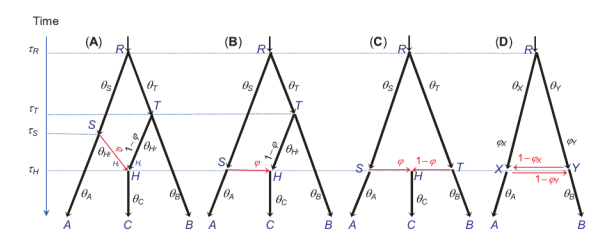
\includegraphics[scale=0.7890]{figures/fig-msci-models}
  \caption{Four different types of MSci models implemented in
    \textsc{bpp}.  The models are
    specified using the extended Newick format, as follows: \\
    \texttt{
      (A): ((A, (C)H[\&phi=0.5,\&tau-parent=yes])S, (H[\&tau-parent=yes], B) T)R; \\
      (B): ((A, (C)H[\&phi=0.5,\&tau-parent=no])S, (H[\&tau-parent=yes], B) T)R; \\
      (C): ((A, (C)H[\&phi=0.5,\&tau-parent=no])S, (H[\&tau-parent=no], B) T)R; \\
      (D): ((A, (B) Y[\&phi=0.3])X, (X[\&phi=0.1])Y)R; \\
      (D): ((A, (B)Y)X, (X)Y)R; \\
      (D): ((A, Y)X, (B, X)Y) R; \\
      (D): ((A, y)x, (B, x) y) r; } } \label{fig-msci-models}
\end{figure}
The control file variable \texttt{phiprior} specifies the prior
probability for the $\varphi$ parameter, which is a beta distribution
with parameters $a$ and $b$.  The syntax is
\begin{verbatim}
phiprior = a b
\end{verbatim}
where $a$ and $b$ are positive numbers. For example, \texttt{phiprior
  = 1 1} specifies the beta prior beta($a, b$) with $a = 1$ and
$b = 1$ for $\varphi$, the introgression probability under the MSci
model.

\chapter{Odds and Ends}


\begin{verbatim}
heredity = 0       # (0: No variation)
heredity = 1 4 4   # (1: estimate, & a_gamma b_gamma)
heredity = 2 heredity.txt      # (2: from file)
\end{verbatim}

\texttt{heredity = 0} is the default and means that $\theta$ is the
same for all loci. \texttt{heredity = 1} or \texttt{2} specifies two
models that allow $\theta$ to vary among loci, which may be useful for
combined analysis of data from autosomal, mitochondrial, X and Y loci.
With such mixed data, the effective population sizes are different
among loci, so that a heredity multiplier \citep[inheritance
scalars][]{Hey2004} should be applied.  Other factors such as natural
selection may also cause $\theta$ to deviate from the neutral
expectation.  \textsc{BPP} implements two options for this.  The first
option (\texttt{heredity = 1}) is to estimate the multipliers from the
data, using a gamma prior with parameters $\alpha$ and $\beta$
specified by the user.  In the example above, a gamma prior $G(4, 4)$,
with mean $4/4 = 1$, is specified for the multiplier for each locus.
The MCMC should then generate a posterior for the multiplier for each
locus.  The second option (\texttt{heredity = 2}) is for the user to
specify the multipliers in a file, and the multipliers will then be
used as fixed constants in the MCMC run.  The file simply contains as
many numerical values as the number of loci, separated by spaces or
line breaks.


\begin{table}
  \centering
  \caption{Heredity scalars}

   \begin{tabular}{lc}
     \toprule \\
     Genome	& Heredity scalar\\
     \midrule \\
     Nuclear  & autosome	1 \\
     X chromosome &	0.75 \\
     Y chromosome & 0.25 \\
     Mitochondrial & 0.25 \\
     \bottomrule
   \end{tabular}  \label{table-heredity-scalar}
 \end{table}

 Note.--- The effect of the locus-specific mutation rates and the
 locus-specific heredity multipliers are different.  A locus rate is
 used to multiply all $\theta$s and $\tau$s for the locus, while a
 heredity multiplier is used to multiply all $\theta$ parameters for
 the locus but not the $\tau$s.  Nevertheless, those parameters are
 quite likely to be strongly correlated, especially when the species
 tree is small.

 \red{Ziheng note on 3 March 2011. The model of sequence errors is
   rewritten, so that the old option is unavailable.  Use
   \texttt{sequenceerror = 0}.}


 \chapter{Methods of Analysis} \label{analysismethods} Here we
 describe the specifics of the four different types of analyses that
 BPP can perform and illustrate them using several of
 the example control files provided in the
 \texttt{examples} subdirectory of the BPP distribution. Briefly, BPP is
 capable of analyzing sequence data using 4 distinct phylogeographical
 models. The 4 models are determined by the combinations of two
 possible settings for each of the two Boolean control file variables
 \texttt{speciesdelimitation} (0 = no species delimitation, 1 =
 species delimitation) and \texttt{speciestree} (0 = fixed species
 tree, 1 = inferred species tree). Therefore, analysis A00 infers the
 biogeographical parameters $\theta$ and $\tau$ on a fixed (user
 specified) tree with a fixed (delimited) number of
 species/populations as described in \cite{Rannala2003}.  Analysis A10
 delimits the number of species and infers biogeographical parameters
 using a fixed species tree (guide tree) as described in
 \cite{Yang2010}.  Analysis A01 infers the species tree and
 biogeographical parameters using a fixed number of species
 (delimitation) as described in \cite{Rannala2017}.  Analysis A11
 jointly infers the species tree, species delimitation and
 biogeographical parameters as described in \cite{Yang2014a}. Under
 Model A00 it is also possible to include a model of either instantaneous
 introgression or ongoing gene flow -- examples of such analyses are given in
 Chapter~\ref{introgression}.
 For each of these 4 major types of analyses the control file specifications
 will differ as well as the form of output printed to the screen and output
 files. Therefore, we will include two subsections in our discussion
 of each analysis method: input and output. Here we only consider the
 control file variables specific to the methods of analysis under
 consideration. For a general discussion of other control file
 variables see the example control file discussed in
 section~\ref{ctrlfile}. Note that for most analyses the output printed
 to screen during the run and that printed to the specified output
 file will be identical.

 It is important to note that only analysis A00 applies within-model inference.
 There is one specified model in that case (the MSC with a fixed species tree)
 and the parameters are well defined, with the objective being to estimate those
 parameters.  In contrast, analyses A01, A10, and A11 all apply trans-model
inference. They move between different models, and the main objective
is to calculate the posterior probabilities of the models.  Each is an
instance of the MSC model, but the species delimitation (the number and
nature of the species) and/or the species phylogeny may differ between models.
In analyses A01, A10, and A11, the prior specified using control file variable
\texttt{thetaprior} applies to all $\theta$ parameters in all models.
Similarly, all MSC models specifying two or more delimited species have a
parameter $\tau_0$ (the divergence time of the root), and these
parameters (for different models) are assigned the same prior,
specified by the \texttt{tauprior} control file variable.

 
 \section{A00: Estimating $\theta$s and $\tau$s} \label{a00} Analysis
 A00\texttt{(speciesdelimitation = 0, speciestree = 0)}, requires a
 user-specified species tree topology, given by variable
 \texttt{species\&tree} in the control file, and infers the $\theta$
 and $\tau$ parameters on this fixed tree.  The theory underlying
 estimation of species divergence times and population sizes ($\tau$s
 and $\theta$s) under the MSC model when the species phylogeny is
 given is described in \citep{Rannala2003}.  Note that if there are
 $s$ species in the species tree, the model will minimally contain the
 following parameters: $s – 1$ species divergence times ($\tau$s) and
 $s – 1$ ancestral species $\theta$s.  A $\theta$ parameter will also
 exist for each contemporary species with at least two sequences
 present at some locus. If the data are for a single
 species/population, the model will contain one parameter only,
 $\theta$ for that species. If there is only one species, the MSC
 model becomes the single-population coalescent
 \citep{Kingman1982}. We will provide examples of both a single
 population analysis (using the control file \texttt{yu2001.bpp.ctl})
 and a multi-species analysis (using the control file
 \texttt{A00.bpp.ctl}).


\begin{mdframed}
  \textbf{How many $\theta$ and $\tau$ parameters exist?} \\
  The number of parameters that \textsc{BPP} includes in the MSC or
  MSci models depends on the data configuration. The program always
  includes $\theta$ and $\tau$ parameters for each internal node
  (ancestral species) on the species tree, but includes a $\theta$ for
  an extant species (tip) if and only if that species has at least 2
  sequences at some loci.  If two or more sequences for a species are
  specified in the control file but there are at most 0 or 1 sequence
  per locus for that species in the sequence data file, $\theta$ for
  that species will not be identifiable or estimable.  In that case,
  the posterior for the parameter will be the prior.  Nevertheless,
  other results (such as the posterior distribution for other
  parameters or posterior probabilities for species trees and species
  delimitations) will still be correct.  The same applies to other
  more complex cases of missing data and parameter non-identifiability.
  As an example, suppose the species tree and the numbers of sequences
  for two kinds of loci are as follows: \\
  ((A,B), (C,D)) \\
  locus configuration 1:  1 1 0 0 \\
  locus configuration 2:  2 0 0 1 \\
  In this case, $\theta_A$, $\theta_{AB}$, $\theta_{ABCD}$,
  $\tau_{AB}$, and $\tau_{ABCD}$ are identifiable while $\theta_B$,
  $\theta_C$, $\theta_D$, $\theta_{CD}$ and $\tau_{CD}$ are not.  Ii
  is impossible to estimate $\theta_D$ , $\theta_{CD}$ and $\tau_{CD}$
  as no data are available from species C.
\end{mdframed}

\subsection{Input A00 (single population)}
Our first example is a dataset of human sequence data generated by
\citet{Yu2001}. The control file is found in the BPP distribution at
location:
\begin{verbatim}
examples/yu2001/yu2001.bpp.ctl
\end{verbatim}
The data comprise 61 phased sequences for a single locus that will be
analyzed to estimate the single parameter $\theta$.  There is no need
to specify an Imap file, or tag the sequence names in the sequence
file (\texttt{yu2001.txt}); the sequence names are read and then
ignored.  Multiple loci may be included in the sequence file. The
contents of the control file \texttt{yu2001.bpp.ctl} are shown below:


\begin{verbatim}
seed = -1

seqfile = yu2001.txt
outfile = out.txt
mcmcfile = mcmc.txt

# fixed species delimitation and species tree
speciesdelimitation = 0 
speciestree = 0

species&tree = 1  H
                  61  

# 0: no data (prior); 1:seq like
usedata = 1

# number of data sets in seqfile
nloci = 1    

# remove sites with ambiguity data (1:yes, 0:no)?
cleandata = 0    

# gamma(a, b) for theta
thetaprior = gamma 2 2000

# auto (0 or 1): finetune for GBtj, GBspr, theta, tau, mix, locusrate, seqerr
finetune = 1: 2 0.00001 0.0001  0.0005 0.5 0.2 1.0  

# MCMC samples, locusrate, heredityscalars, genetrees, locussubstitution
print = 1 0 0 0  

burnin = 4000
sampfreq = 2
nsample = 10000
\end{verbatim}

\noindent
The two lines:
\begin{verbatim}
speciesdelimitation = 0 
speciestree = 0
\end{verbatim}
specify that the species delimitation (number of species) is fixed as
well as the species tree topology. In this case,
there is no species tree and only a single species exists.  There is
no need for a species tree, so the block for specifying species names
and species tree looks like this:
\begin{verbatim}
species&tree = 1  H
                  61
\end{verbatim}
\noindent
The line:
\begin{verbatim}
# gamma(a, b) for theta
thetaprior = gamma 2 2000
\end{verbatim}
specifies a gamma distribution for the prior on $\theta$ with
parameters $\alpha = 2$ and $\beta = 2000$ which has mean $0.001$ and
variance $5 \times 10^{-7}$.

\subsection{Output A00 (single population)}
When BPP is run using the above control file a summary of the progress
of the MCMC analysis is printed to screen. Here, we briefly explain what
this output means. The different analyses presented in this chapter
all produce a similar form of output when the program is running, but
the number of columns and their specific content varies somewhat.
Omitting some mostly irrelevant output related to the adjustment of
proposal moves, the output to screen when this control file is run
appears as follows:
\begin{verbatim}
     |  Acceptance proportions  |
Prgs | Gage Gspr thet  tau  mix | mthet1       log-PG         log-L
-------------------------------------------------------------------
 -15%  0.71 0.18 0.30 0.00 0.38   0.0004    467.11472  -12721.22305  0:01
 (some output omitted here)
   5%  0.71 0.29 0.33 0.00 0.24   0.0004    428.40742  -12721.09413  0:05
  10%  0.71 0.29 0.31 0.00 0.25   0.0003    480.92848  -12720.75185  0:06
  15%  0.71 0.29 0.30 0.00 0.24   0.0003    476.37432  -12720.65199  0:08
  20%  0.71 0.29 0.31 0.00 0.23   0.0003    441.36960  -12720.92326  0:09
  25%  0.71 0.29 0.32 0.00 0.23   0.0003    443.51740  -12720.85802  0:10
  30%  0.71 0.29 0.31 0.00 0.23   0.0003    441.93616  -12720.86033  0:11
  35%  0.71 0.29 0.31 0.00 0.23   0.0003    495.50716  -12720.84565  0:12
  40%  0.71 0.29 0.31 0.00 0.23   0.0003    452.82049  -12720.87810  0:13
  45%  0.71 0.29 0.31 0.00 0.23   0.0003    461.93346  -12720.94582  0:15
  50%  0.71 0.29 0.32 0.00 0.23   0.0004    463.85955  -12721.01005  0:16
  55%  0.71 0.29 0.32 0.00 0.23   0.0004    463.42744  -12720.98006  0:17
  60%  0.71 0.29 0.32 0.00 0.23   0.0004    478.52797  -12721.03353  0:18
  65%  0.71 0.29 0.32 0.00 0.23   0.0004    499.97705  -12720.96168  0:19
  70%  0.71 0.29 0.32 0.00 0.23   0.0004    455.32489  -12720.93611  0:20
  75%  0.71 0.29 0.32 0.00 0.23   0.0004    439.21544  -12720.99190  0:22
  80%  0.71 0.29 0.32 0.00 0.23   0.0004    461.56954  -12721.00180  0:23
  85%  0.71 0.29 0.32 0.00 0.23   0.0004    469.53443  -12720.99823  0:24
  90%  0.71 0.29 0.32 0.00 0.23   0.0004    455.60303  -12720.99213  0:25
  95%  0.71 0.29 0.32 0.00 0.23   0.0004    454.07141  -12721.00745  0:26
 100%  0.71 0.29 0.32 0.00 0.23   0.0004    461.01044  -12720.97549  0:27

0:27 spent in MCMC

          theta_1H	lnL
mean      0.000352  -12720.995649
median    0.000337  -12720.726000
S.D       0.000116  2.936769
min       0.000089  -12735.535000
max       0.001293  -12712.774000
2.5%      0.000170  -12727.454000
97.5%     0.000617  -12716.086000
2.5%HPD   0.000145  -12726.920000
97.5%HPD  0.000574  -12715.718000
ESS*      757.838791  1180.434956
Eff*      0.075784  0.118043
\end{verbatim}

\noindent
The line:
\begin{verbatim}
     |  Acceptance proportions  |
Prgs | Gage Gspr thet  tau  mix | mthet1       log-PG         log-L
-------------------------------------------------------------------
\end{verbatim}

\noindent
is a header that explains the content of each column printed during
the run.  The \texttt{Prgs} (progress) column will appear in all
analyses and indicates the percentage of the MCMC iterations that have
been completed. If this number is negative it indicates that the
program is still running the burn-in iterations.  For example,
\texttt{-15\%} means that 15 percent of the burn-in iterations remain
to be completed. The next 5 columns are the current acceptance
proportions for different parameter proposals in the MCMC. The
proposals are defined as follows:
\begin{itemize}
\item \texttt{Gage}: proposal to change ages of nodes on gene trees
\item \texttt{Gsbr}: proposal to change gene tree topology using SPR
  move
\item \texttt{thet}: proposal to change $\theta$ parameter
\item \texttt{tau}: proposal to change $\tau$ parameter
\item \texttt{mix}: mixing step proposal
\end{itemize}
In the output the acceptance proportions are stable. The fifth column
(the $\tau$ proposal acceptance proportion) is zero; this is expected
because there are no species divergence times ($\tau$s) in the model
when only a single species exists.  Column 7, labeled \texttt{mthet1}
gives the current average (mean) value of theta in the MCMC.  Columns
8 and 9 are the log probability of the coalescent model
(\texttt{log-PG}) and the log-likelihood of the sequence data on the
gene tree (\texttt{log-L}). Check that the acceptance proportions are
in a reasonable range (about 20\% to 40\% for continuous parameters
such as $\theta$). If you need to terminate the program before it
finishes, you can do so using the key combination {\color{red}\texttt{Ctrl-C}}
(e.g., hold down the Control key and then press the C key).
The final screen output, printed after the MCMC is
completed, summarizes the posterior parameter estimates for $\theta$
(\texttt{theta\_1H}) in the second column. The posterior mean in the
first row, for example, is $0.000352$ and the lower and upper limits
of the highest posterior density (HPD) set of values are in rows 8 and
9, respectively. In this case, the HPD credibility interval for
$\theta$ is $(0.000145,0.000574)$.

\subsection{Input A00 (multiple populations)}
Our second example is a dataset of frog sequence data generated by \cite{Zhou2012}.
This same dataset will also be used to illustrate analyses A01, A10 and A11.
The control file is found in the BPP distribution at location:
\begin{verbatim}
examples/frogs/A00.bpp.ctl
\end{verbatim}
The data comprise 5 loci for 4 populations, with the number of sequences at each locus varying
between 21 and 30. We will be estimating $\theta$s for each of the 4 contemporary and 3 ancestral populations
as well as the 3 species divergence times ($\tau$s). The contents of the control file
\texttt{A00.bpp.ctl} are shown below:

\begin{verbatim}
seed =  -1

seqfile = frogs.txt
Imapfile = frogs.Imap.txt
outfile = out.txt
mcmcfile = mcmc.txt

# fixed number of species/populations
speciesdelimitation = 0 

# fixed species tree
speciestree = 0

species&tree = 4  K  C  L  H
                    9  7 14  2
                 (((K, C), L), H);

# unphased data for all 4 populations
phase =   1  1  1  1

# use sequence likelihood                  
usedata = 1

nloci = 5  

# do not remove sites with ambiguity data
cleandata = 0    

# gamma(a, b) for theta (estimate theta)
thetaprior = gamma 2 2000 

# invgamma(a, b) for root tau & Dirichlet(a) for other tau's
tauprior = invgamma 3 0.002 

# finetune for GBtj, GBspr, theta, tau, mix, locusrate, seqerr
finetune =  1: 5 0.001 0.001  0.001 0.3 0.33 1.0  

# MCMCsamples, locusrate, heredityscalars, genetrees, substitutionparams
print = 1 0 0 0 0   

burnin = 8000
sampfreq = 2
nsample = 100000
\end{verbatim}

\noindent
As in the previous analysis, the two lines:
\begin{verbatim}
speciesdelimitation = 0 
speciestree = 0
\end{verbatim}
specify that the species delimitation (number of species) is fixed as
well as the species tree topology. In this case,
a species tree is specified along with population labels.
The block for specifying species names
and the species tree looks like this:

\begin{verbatim}
species&tree = 4  K  C  L  H
                    9  7 14  2
                 (((K, C), L), H);
\end{verbatim}

\noindent
The first line above lists the number of species (populations) which is
4 in this example. This is followed
by the label for each species (these should match the labels in the map
file):
\begin{verbatim}
K  C  L  H
\end{verbatim}
The next line specifies the maximum number of sequences per
species in the same order as the species labels:
\begin{verbatim}
9  7 14  2
\end{verbatim}
the actual number of sequences at any locus must be less than this value.
The third line is a rooted phylogenetic tree topology specified in
Newick format:
\begin{verbatim}
(((K, C), L), H);
\end{verbatim}
The next line specifies that the loci for each of the 4 populations
are unphased:
\begin{verbatim}
phase = 1 1 1 1
\end{verbatim}
The specified phase variables should include a 0 or 1 (Boolean) entry for each population, 
where the populations are assumed to be in the same order as specified above
(in the \texttt{species\&tree} block)
and the Boolean variable indicates that the sequence data for a population
are either unphased (1) or phased (0). Ambiguity characters are used to represent
genotypes for unphased sequences (see Section~\ref{controlfilevariables}).
In the example data the sequences are unphased for all 4 populations.
Currently, it is not possible to have partially phased data (e.g., only
some loci unphased in a particular population). The program will infer
the phase as part of the analysis.

Unlike the earlier single population analysis, in which we estimated a
single $\theta$ parameter, in the multipopulation analysis we will be
estimating multiple $\theta$s (one for each population) and divergence
times ($\tau$s) between populations. Thus, we have prior distributions
for both $\theta$ and $\tau_0$. The lines below specify a gamma distribution
as the prior for $\theta$ with parameters $\alpha = 2$ and $\beta = 2000$
(the prior mean and variance of $\theta$ are $0.001$ and $0.0000005$):
\begin{verbatim}
# gamma(a, b) for theta
thetaprior = gamma 2 2000 
\end{verbatim}
The lines:
\begin{verbatim}
# invgamma(a, b) for root tau & Dirichlet(a) for other tau's
tauprior = invgamma 3 0.002 
\end{verbatim}
specify an inverse gamma distribution as a prior for
the root age and the remaining $\tau$s have a uniform Dirichlet
distribution conditional on the root age (the prior mean and variance of the
root age are $0.001$ and $0.000001$,respectively):

\newpage
\subsection{Output A00 (multiple populations)}
When BPP is run using the above control file a summary of the progress of the
MCMC is again printed to screen as follows:
{ \scriptsize
\begin{verbatim}
     |  Acceptance proportions  |
Prgs | Gage Gspr thet  tau  mix | mthet1 mthet2 mthet3   mtau1  mtau2  mtau3       log-PG        log-L
------------------------------------------------------------------------------------------------------
  -3%  0.65 0.10 0.43 0.04 0.12   0.0031 0.0095 0.0068  0.0021 0.0015 0.0014   1204.63468  -4458.38814
 (some output omitted here)
   5%  0.64 0.26 0.30 0.28 0.27   0.0035 0.0096 0.0067  0.0019 0.0018 0.0017   1225.51650  -4443.85539  1:09
  10%  0.65 0.27 0.30 0.28 0.28   0.0035 0.0095 0.0068  0.0019 0.0018 0.0018   1202.62497  -4445.50020  1:47
  15%  0.64 0.27 0.30 0.28 0.28   0.0034 0.0095 0.0068  0.0019 0.0018 0.0017   1211.95125  -4446.35694  2:25
  20%  0.64 0.26 0.31 0.28 0.28   0.0034 0.0095 0.0067  0.0018 0.0018 0.0017   1211.09206  -4445.74292  3:05
  25%  0.64 0.26 0.31 0.28 0.28   0.0034 0.0096 0.0067  0.0018 0.0018 0.0017   1222.97603  -4446.12020  3:43
  30%  0.64 0.26 0.31 0.28 0.28   0.0034 0.0096 0.0067  0.0018 0.0018 0.0017   1216.60217  -4445.55424  4:21
  35%  0.64 0.26 0.31 0.28 0.28   0.0034 0.0096 0.0067  0.0018 0.0018 0.0017   1260.59722  -4445.22113  5:00
  40%  0.64 0.26 0.31 0.28 0.27   0.0034 0.0096 0.0067  0.0018 0.0018 0.0017   1269.45020  -4445.20340  5:38
  45%  0.65 0.26 0.31 0.28 0.27   0.0034 0.0096 0.0067  0.0018 0.0018 0.0017   1243.07668  -4445.00207  6:16
  50%  0.65 0.26 0.31 0.28 0.27   0.0034 0.0096 0.0067  0.0018 0.0018 0.0017   1229.59858  -4445.04036  6:55
  55%  0.64 0.26 0.31 0.28 0.27   0.0034 0.0096 0.0067  0.0018 0.0018 0.0017   1209.31273  -4445.43161  7:33
  60%  0.64 0.26 0.31 0.28 0.27   0.0034 0.0096 0.0067  0.0018 0.0018 0.0017   1206.22162  -4445.53994  8:11
  65%  0.64 0.26 0.31 0.28 0.27   0.0034 0.0096 0.0067  0.0018 0.0018 0.0017   1190.78837  -4445.21618  8:50
  70%  0.64 0.26 0.31 0.28 0.27   0.0034 0.0096 0.0067  0.0018 0.0018 0.0017   1203.82684  -4445.04124  9:30
  75%  0.64 0.26 0.31 0.28 0.27   0.0034 0.0096 0.0067  0.0018 0.0018 0.0017   1186.32176  -4445.00578  10:09
  80%  0.64 0.26 0.31 0.28 0.27   0.0034 0.0096 0.0067  0.0018 0.0018 0.0017   1222.75718  -4444.94315  10:47
  85%  0.64 0.26 0.31 0.28 0.27   0.0034 0.0096 0.0067  0.0018 0.0018 0.0017   1228.39106  -4444.68671  11:26
  90%  0.64 0.26 0.31 0.28 0.27   0.0034 0.0096 0.0067  0.0018 0.0018 0.0017   1228.72385  -4444.54844  12:04
  95%  0.64 0.26 0.31 0.28 0.27   0.0034 0.0096 0.0067  0.0018 0.0018 0.0017   1223.25921  -4444.25455  12:43
 100%  0.64 0.26 0.31 0.28 0.27   0.0034 0.0096 0.0067  0.0018 0.0018 0.0017   1199.52731  -4444.17857  13:21
}
13:21 spent in MCMC

          theta_1K  theta_2C  theta_3L	theta_4H  theta_5KCLH theta_6KCL theta_7KC tau_5KCLH tau_6KCL tau_7KC lnL
mean      0.003422  0.009588  0.006683  0.003031  0.003720  0.001577  0.001648  0.001823  0.001787  0.001710  -4444.16
median    0.003351  0.009492  0.006599  0.002932  0.003642  0.001412  0.001463  0.001809  0.001773  0.001700  -4443.69
S.D       0.000747  0.001461  0.001118  0.000819  0.000944  0.000899  0.000954  0.000234  0.000230  0.000238  11.615936
min       0.001309  0.004913  0.003258  0.000866  0.001131  0.000029  0.000039  0.001047  0.001043  0.000772  -4496.72
max       0.008147  0.017569  0.012778  0.009724  0.010355  0.008461  0.008987  0.003140  0.003113  0.002847  -4403.99
2.5%      0.002171  0.006999  0.004743  0.001729  0.002100  0.000325  0.000340  0.001404  0.001375  0.001271  -4468.01
97.5%     0.005084  0.012720  0.009104  0.004919  0.005780  0.003751  0.003991  0.002319  0.002280  0.002209  -4422.74
2.5%HPD   0.002071  0.006802  0.004595  0.001566  0.001949  0.000142  0.000164  0.001396  0.001342  0.001252  -4467.06
97.5%HPD  0.004928  0.012469  0.008903  0.004650  0.005573  0.003312  0.003512  0.002308  0.002237  0.002185  -4421.90
ESS*      2721.25   8954.56   5279.29   11762.38  1199.63   4543.27   3299.32   850.33    970.61    932.00    420.40
Eff*      0.027213  0.089546  0.052793  0.117624  0.011996  0.045433  0.032993  0.008503  0.009706  0.009320  0.004204

\end{verbatim}
}
There are again 5 acceptance proportions for the 5 parameter proposals, but now the current mean values of 6
parameters are printed. The current mean values of $\theta$ for nodes 1, 2 and 3 (\texttt{mthet1 mthet2 mthet3})
are printed -- which are $\theta$s of the contemporary species K, C and L, and those of
the 3 $\tau$s (\texttt{mtau1  mtau2  mtau3}) which are the divergence times for ancestral species
KCLH, KCL and KC, respectively. If there are many populations/species only the first few $\tau$s will be printed to
screen but all the $\tau$s will be available in the summary created at the end of the run (see below).
When the run finishes, a final block is written summarizing the results. The first two
rows give the mean and median of the posterior distribution for each parameter. This is followed by
summaries of the statistical uncertainty: the standard deviation (S.D.) of the posterior distribution;
the minimum (min) and maximum (max) values; the lower and upper bounds of the 95\%
\href{https://en.wikipedia.org/wiki/Credible_interval}{Credible Interval} (2.5\% and 97.5\%);
the lower and upper bounds of the \href{https://en.wikipedia.org/wiki/Credible_interval}{Highest Posterior Density (HPD) Interval} (2.5\%HPD and 97.5\%HPD);
the Effective Sample Size (ESS*); and the Efficiency (Eff*). Larger values for ESS* and Eff* indicate better
mixing and more reliable estimates.
The above information is also printed (along with other technical details of the run)
to the output file specified by the \texttt{outfile} variable in the control file (in our example, \texttt{out.txt}).
A tree file in NEXUS/Newick format is also created and placed in the file named FigTree.tre which is formatted
for viewing/printing using the \href{http://tree.bio.ed.ac.uk/software/figtree/}{Figtree} program

\subsection{MCMC output file}
A file will be produced (with a name specified by the control file variable \texttt{mcmcfile}) that contains the mcmc samples from the run for
all the $\theta$ and $\tau$ parameters. When running under analysis method A00 the contents of this file can be analyzed using a program
such as \href{}{Tracer} to visually examine the convergence and mixing of the MCMC run. However, the other three analysis methods (A01, A10 and A11) are trans-model analyses in which the number of parameters and or/the meaning of the parameters changes as the chain runs so it is not
correct to examine the trace plot without conditioning on a particular model.

\subsection{Adjusting step lengths for MCMC moves (finetune)}

You can use the automatic adjustment of the finetune variable (MCMC
step lengths), which appears to be reliable, but make sure that the
acceptance proportions are neither too small nor too large.  Below are
notes for manual adjustments of the step lengths.  Often I use
automatic adjustments to generate good step lengths and then copy them
into the control file, so that the next time the automatic procedure
starts with already good step lengths.

Below are some notes about adjusting the step lengths manually
(finetune = 0).

First note the following line in the control file ChenLi2001.bpp.ctl.
Here finetune = 0 means that MCMC step lengths will not be adjusted
automatically, and they are used as given.
\begin{verbatim}
finetune = 0: .01 .02 .03 .04 .05 .01 .01  # auto (0 or 1): MCMC step lengths
\end{verbatim}
There are seven finetune steplengths here.  They are in a fixed order
and always read by the program even if the concerned proposal is not
used.  The first five of them are $\epsilon_1$, $\epsilon_2$,
$\epsilon_3$, $\epsilon_4$, and $\epsilon_5$, described in
\citep{Rannala2003}. These are the step lengths used in the MCMC
proposals that (1) change internal node ages in the gene tree, (2)
prune and re-graft nodes in the gene tree, (3) update $\theta$, (4)
update $\tau$s using the rubber-band algorithm, and (5) implements the
mixing step.  The 6th and 7th are for the proposals that change the
locus rates or heredity multipliers and that change the sequencing
errors, respectively.  If the model assumes the same rate for all loci
and does not use heredity multipliers, the 6th proposal step is not
used.  If the model assumes no sequencing errors, the 7th step is not
used.  The acceptance proportions for the first five proposals are
always printed out on the screen, but those for the 6th and 7th are
printed out only if the concerned proposal is used in the model.  In
the example above, only the first five proposals are used in the
algorithm and we will change the step lengths so that the acceptance
proportions become close to 30\%.  If the acceptance proportion is too
small (say, <0.10)), decrease the corresponding finetune parameter.
If the acceptance proportion is too large (say, >0.80), increase the
finetune parameter.

Run the program for a small number of iterations and look at the
screen output for the acceptance proportions.
{\small
\begin{verbatim}
lnpG0 = 2440.0952  lnL0 = -43946.6769
 0% 0.13 0.00 0.00 0.04 0.43  0.0009 0.0009 0.0008  0.0150 0.0067 0.0057 2399.70 -43752.8348  0:05
 5% 0.14 0.00 0.00 0.04 0.44  0.0009 0.0009 0.0008  0.0148 0.0064 0.0057 2340.71 -43738.0172  0:09
10% 0.14 0.00 0.00 0.04 0.44  0.0009 0.0009 0.0008  0.0149 0.0064 0.0056 2383.91 -43739.3830  0:14
\end{verbatim}
}
Here the second acceptance proportion, at 0.00, is much too small,
which means that the corresponding step-length (0.02 in the control
file) is much too large.  Terminate the run (Ctrl-C) and decrease the
value in the control file.  Then run the program again (use the up and
down arrow keys to retrieve past commands).  Repeat this process a few
times until every acceptance proportion is neither too small nor too
large.  In this example, changing 0.02 to 0.002 brings the acceptance
proportion to ~24\%, which is slightly too small but already good
enough.

Those MCMC proposals are used in all four analyses (A00, A01, A10,
A11), so that the description here applies to all of them.  Note that
the finetune parameters affect the efficiency of the MCMC or how fast
one can obtain reliable results.  In theory they do not change the
results if all runs using different finetune parameters are long
enough to generate reliable results.





\newpage

\texttt{A01} means species tree estimation when the assignments and
delimitation are fixed.
\begin{verbatim}
speciesdelimitation = 0    *
speciestree = 1    * NNI/SPR over species trees
speciesmodelprior = 1  * 0: uniform LH; 1:uniform rooted trees; 2: uniformSLH; 3: uniformSRooted
\end{verbatim}

This invokes the NNI or SPR algorithm to change the species tree
topology, while species delimitation is fixed (so that the number of
species and the assignment of individuals to species are fixed).

A10, for species delimitation using a user-specified guide tree
\citep{Yang2010, Rannala2013}, is specified using

\begin{verbatim}
speciesdelimitation = 1 0 2   * speciesdelimitation algorithm0 and finetune(e)
speciesdelimitation = 1 1 2 1 * speciesdelimitation algorithm1 finetune (a m)
speciesmodelprior = 1  * 0: uniform LH; 1:uniform rooted trees
\end{verbatim}

The first line specifies rjMCMC algorithm 0, with $\epsilon = 2$ in
equations 3 and 4 of \cite{Yang2010}.  Reasonable values for
$\epsilon$ are 1, 2, 5, etc. \\ The second line specifies rjMCMC
algorithm 1, with $ \alpha = 2$ and $m = 1$ in equations 6 and 7 of
\cite{Yang2010}. Reasonable values are $\alpha = 1, 1.5, 2$, etc. and
$m = 0.5, 1, 2$, etc.

The two algorithms in theory should produce identical results.  The
variable \texttt{speciesmodelprior} specifies Priors 0 and 1.  Prior 0
means equal probabilities for labeled histories (which are rooted
trees with internal nodes ordered by their age).  This is the prior
used by \cite[][eq.~2]{Yang2010}.  Prior 1 means equal probabilities
for rooted trees.  This is now the default.  The prior with the user
specified probabilities for nodes described by \cite{Rannala2013} is
deleted since version 2.3(?).

\texttt{A11}, for joint species delimitation and species tree
inference or for unguided species delimitation \cite{Yang2014a}, is
specified as follows.
\begin{verbatim}
speciesdelimitation = 1 0 2    * rjMCMC speciesdelimitation algorithm0(e)
*speciesdelimitation = 1 1 2 1  * rjMCMC speciesdelimitation algorithm1(a m)
speciestree = 1    * NNI over species trees
speciesmodelprior = 1  * 0: uniform LH; 1:uniform rooted trees; 2: uniformSLH; 3: uniformSRooted
\end{verbatim}

In this case, \textsc{bpp} will use the rjMCMC algorithm (either
algorithm 0 or algorithm 1 of \cite{Yang2010} to change the species
delimitation model and the NNI/SPR move to change the species tree
topology.

For A11, \texttt{speciesmodelprior} can take the four values 0, 1, 2,
3, which mean Priors 0, 1, 2, 3, respectively.  As mentioned above,
Prior 1 (which is the default) assigns equal probabilities to the
rooted species trees, while Prior 0 means equal probabilities for the
labeled histories (rooted trees with the internal nodes ordered by
age).  Priors 2 and 3 assign equal probabilities for the numbers of
species (1/s each for 1, 2, ..., s species given s populations) and
then divided up the probability for any specific number of species
among the compatible models (of species delimitation and species
phylogeny) either uniformly [Prior 3] or in proportion to the labeled
histories [Prior 2].  Priors 2 and 3 are mentioned by \cite{Yang2014a}
and implemented by \cite{Yang2015}.  Prior 3 may be suitable when
there are many populations.





\section{A01: Species Tree Estimation}

Suppose we use the control file bpp.4s.ctl to run analysis A01:
species tree estimation with species delimitation and assignment fixed
(speciesdelimitation = 0, speciestree = 1).

The screen output will look like this:

\begin{verbatim}
 5% 0.28 0.28 0.28 0.35 0.29  0.0000  0.0033 0.0138 2403.43 -43721.0651  0:13
10% 0.27 0.27 0.27 0.36 0.30  0.0000  0.0028 0.0142 2304.08 -43723.0804  0:21
15% 0.26 0.27 0.26 0.36 0.30  0.0000  0.0025 0.0143 2308.11 -43723.8564  0:27
  ^^ Pjump for MCMC moves ^^  PSPR   theta  tau     lnpG    E(lnL)
\end{verbatim}

Here the five Pjump values are the acceptance proportions for the five
conventional MCMC moves, as discussed above.  PSPR is the acceptance
proportion for the SPR/Nodeslider moves that change the species
phylogeny \cite{Rannala2017}.  The next two numbers are posterior
means of $\theta$ for the root population (-1 is printed if $\theta$s
are integrated out) and $\tau_0$ for the root age.  The last two
numbers are the log MSC gene-tree density \citep{Rannala2003} and the
average log sequence likelihood \cite{Felsenstein1981}.

\textbf{The MCMC sample} of species trees is collected in the file
mcmc.txt.  Below are two lines from that file.  The numbers after :
are the branch lengths ($\tau$s), while those after \# are $\theta$s.
I hope to change the output format to be more consistent with the
Newark format.

\begin{verbatim}
(((H #0.000708: 0.004728, C #0.000740: 0.004728) #0.002814: 0.001190, G #0.000574: 0.005918) #0.004132: 0.007626, O #0.002036: 0.013544) #0.003835;
(((H #0.000708: 0.004728, C #0.000740: 0.004728) #0.002814: 0.001190, G #0.000574: 0.005918) #0.003740: 0.007351, O #0.002786: 0.013268) #0.003506;
\end{verbatim}

The \textsc{bpp} summary of the sample will look like the following.
\begin{verbatim}
Read tree sample, count trees & splits
tree 20000  (((H, C), G), O);
20001 trees read, 1 distinct trees.

Species in order:
1. H
2. C
3. G
4. O

(A) Best trees in the sample (1 distinct trees in all)
20001  1.00000  1.00000  (O, (G, (H, C)));

(B) Best splits in the sample of trees (2 splits in all)
20001   1.00000  1100
20001   1.00000  1110

(C) Majority-rule consensus tree
(O, (G, (H, C) #1.000000) #1.000000);

(D) Best tree (or trees from the mastertree file) with support values
(O, (G, (H, C) #1.000000) #1.000000);  [P = 1.00000]
\end{verbatim}

Section (A) lists the species trees in decreasing order of posterior
probabilities.  From this you can easily identify the 95\% or 99\%
credibility set of species trees.  Section (B) lists the splits (or
bipartitions) and their posterior probabilities.  The splits here take
into account the location of the root, and may be different from the
splits for unrooted trees.  Section (C) prints the majority-rule
consensus tree, with posterior probabilities for nodes.


\subsection{A10: species delimitation using rjMCMC}

We apply rjMCMC algorithm to the frogs data (A10:
\texttt{speciesdelimitation = 1, speciestree = 0}).
\begin{verbatim}
cd frogs\r1
..\..\bin\bpp ..\A10.bpp.ctl
\end{verbatim}
\textbf{The screen output} will look like the following.  The species
delimitation models that can be generated from the fixed guide tree
are listed, together with their prior probabilities calculated by
\textsc{bpp}.  (As a check, if you use \texttt{usedata = 0}, the MCMC
should be sampling from this prior distribution.)  The species
delimitation model is represented using four 0-1 flags for the four
interior nodes 6, 7, 8, 9 in the guide tree, with 0 for ‘collapsed’
and 1 for ‘resolved’.  Note that the tips in the guide tree are
numbered 1, 2, $\cdots, s$ for $s$ potential species, while the
interior (ancestral) nodes are numbered
$s + 1, s + 2, \cdots, 2s – 1$, with $s + 1$ to be the root of the
guide tree.  The numbering is through a tree-traversal algorithm,
fixed by the program.  This same order is used to specify the
divergence time parameters ($\tau$s), so you can work out the order by
looking at the list of nodes in the screen output (look at the
``population by population table'', ``\# species divergence times in
the order:'', etc.).
\begin{adjustwidth}{-100pt}{100pt}
{\small
\begin{verbatim}
Number of species-delimitation models =  5
delimitation model   1: 000  prior  0.20000
delimitation model   2: 100  prior  0.20000
delimitation model   3: 101  prior  0.20000
delimitation model   4: 110  prior  0.20000
delimitation model   5: 111  prior  0.20000

[Note: Ancestral nodes in order:   5 KCLH  6 KC  7 LH]

MCMC settings: 8000 burnin, sampling every 2, 100000 samples
Approximating posterior, using sequence data
(Settings: cleandata=1 print=1 saveconP=1 moveinnode=1)

Starting rjMCMC...
PrSplit = 0.500000
rj algorithm 1: new theta from G(a=2.00, m=1.00)

Starting species-delimitation model: 111

root dist = 0.00095

Initial parameters, np = 3.
Genetrees generated from the MSC density.
0.00108  0.00074  0.00075
lnpG0 =  752.4533  lnL0 = -3402.2670
-3% 0.70 0.13 0.00 0.20 0.36   3 0.0198 111 P[5]=0.8750  -1.0000 0.0007  787.23 -3127.1399
(nsteps = 5)
Current Pjump:      0.69618  0.13189  0.00000  0.19758  0.35650
Current finetune:   5.00000  0.00100  0.00100  0.00100  0.30000
New     finetune:  18.97702  0.00041  0.00001  0.00063  0.36913

-2% 0.70 0.30 0.00 0.19 0.27   3 0.0209 111 P[5]=0.8575  -1.0000 0.0007  775.05 -3125.7744
(nsteps = 5)
Current Pjump:      0.69565  0.29861  0.00000  0.18742  0.27050
Current finetune:  18.97702  0.00041  0.00001  0.00063  0.36913
New     finetune:  71.87933  0.00041  0.00000  0.00037  0.32779

-1% 0.70 0.31 0.00 0.20 0.33   3 0.0126 111 P[5]=0.8990  -1.0000 0.0007  732.14 -3126.0675
(nsteps = 5)
Current Pjump:      0.69528  0.30537  0.00000  0.20442  0.33250
Current finetune:  71.87933  0.00041  0.00000  0.00037  0.32779
New     finetune:  99.00000  0.00042  0.00000  0.00024  0.37030

 0% 0.69 0.30 0.00 0.23 0.26   3 0.0165 111 P[5]=0.9215  -1.0000 0.0007  723.36 -3125.7568  0:11

(nsteps = 5)
Current Pjump:      0.69354  0.29812  0.00000  0.23367  0.26400
Current finetune:  99.00000  0.00042  0.00000  0.00024  0.37030
New     finetune:  99.00000  0.00042  0.00000  0.00018  0.31993

 5% 0.70 0.30 0.00 0.29 0.34   2 0.0260 110 P[5]=0.8731  -1.0000 0.0007  773.34 -3125.8363  0:25
10% 0.70 0.30 0.00 0.30 0.34   3 0.0234 111 P[5]=0.8778  -1.0000 0.0007  745.39 -3125.8263  0:39
15% 0.70 0.30 0.00 0.30 0.34   2 0.0225 110 P[5]=0.8879  -1.0000 0.0007  762.56 -3125.9276  0:53

^^ Pjump for MCMC moves ^^       Prj      P[model 5]     theta    tau   lnpG     E(lnL)
\end{verbatim}
}
\end{adjustwidth}

The starting species delimitation model is generated by choosing at
random one of the models defined by the guide tree or starting tree.

After the chain has started, the five ratios after the \% sign are the
acceptance proportions for the conventional MCMC moves discussed
above.

Next there are three numbers related to the rjMCMC move, highlighted
in red above.  The rest of the line shows the posterior mean for
$\theta$ for the root and posterior mean for $\tau_0$ (which exist in
all species-tree or species delimitation models), the current log MSC
density and average log sequence likelihood The three numbers related
to the rjMCMC move, ``2 0.0225 110'' in the example, mean that the
current model is 110 (using the flags of fig.  1 in Yang and Rannala,
2010), and the rjMCMC move has the acceptance proportion 0.0225.
[What does the number 2 mean?]  In general the larger this proportion,
the more efficient the rjMCMC algorithm is.  However there is no
optimal acceptance proportion for the rjMCMC move, and a value close
to 0 may not necessarily mean a problem.  If one model has posterior
probability close to 1, the acceptance proportion should be near 0 as
well.  Thus both poor mixing of the rjMCMC algorithm and extreme
posterior model probabilities can cause the acceptance proportion for
the rjMCMC to be close to 0.  It has been noted that if the rjMCMC
algorithm is suffering from poor mixing, different starting species
trees often lead to different results.

Next the posterior probability for the best species-tree model (the
most frequently visited tree model up to now) is printed.  In the
example, ``P[5]=0.8879'' means tree model 5 (111) is the most favoured
model, with the posterior at 0.8879.

After the MCMC is finished, the program will summarize the sample.
The output looks like the following.  The seven delimitation models
are listed again, together with their posterior and prior
probabilities.

\begin{verbatim}
Summarizing the species-delimitation sample in file mcmc.txt

Number of species-delimitation models =  5
model    prior  posterior
1  000   0.20000   0.00000
2  100   0.20000   0.00000
3  101   0.20000   0.00038
4  110   0.20000   0.10019
5  111   0.20000   0.89943

[Note: Ancestral nodes in order:   5 KCLH  6 KC  7 LH]

Guide tree with posterior probability for presence of nodes
((K, C) #0.999620, (L, H) #0.899810) #1.000000;
\end{verbatim}
The MCMC sample file mcmc.txt.  As the number of parameters changes
when the rjMCMC moves between models, the mcmc sample file may not be
very useful, so you can ignore it.  Right now the header line is
generated using the starting species tree and should be ignored.
After the header line, each line of output has the following numbers,
separated by TABs: iteration number, the number of parameters, the
tree, the sampled parameter values, and lnL.  {\small
\begin{verbatim}
Gen	np	tree	tau_5KCLH	tau_6KC	tau_7LH	lnL
2	3	111	0.00079675	0.0007372	0.00065989	-3122.248
4	3	111	0.00074995	0.00067776	0.00059457	-3122.427
...
786	3	111	0.00037556	0.00010047	2.5634e-05	-3129.184
788	3	111	0.00065693	7.9848e-05	3.6489e-05	-3116.988
790	2	110	0.00044831	5.7933e-05	-3125.574
792	2	110	0.00060611	0.00029978	-3122.610
794	2	110	0.00060611	0.00048884	-3122.912
796	2	110	0.00041675	0.00027494	-3130.812
798	2	110	0.00034214	0.0002618	-3142.615
800	3	111	0.00044038	0.00033698	9.8583e-05	-3129.386
802	3	111	0.00060202	0.00047807	7.7594e-05	-3121.725
\end{verbatim}
} If you know the unix command grep, you can retrieve the lines for
the same tree model to summarize the posterior for parameters in that
model.

{\small
\begin{verbatim}
grep "3 111" mcmc.txt > result.Tree111.txt
\end{verbatim}
} In theory this should give you the same posterior as if you run
analysis A00 with the species tree fixed at tree 111.  In practice I
think it is simpler that you edit the Imap file and the control file
to run analysis A00.

\begin{mdframed}
  \textbf{Running rjMCMC Algorithms.}
  \begin{itemize}
  \item The rjMCMC algorithms for species delimitation allow the chain
    to move from one model to another but can have mixing problems.
    Check that similar results are produced from multiple runs using
    Algorithm0 and Algorithm1 regardless of the starting species tree.

    The starting tree is chosen by the program at random and will vary
    among runs.  Make sure that some of your runs are started with the
    one-species model, some from the fully resolved tree, and some
    from other trees in between.  If you get consistent results among
    runs with different starting trees and using the two algorithms,
    you are unlikely to have a convergence or mixing problem.

    If you have a computer with multicore, you can run those different
    combinations or replicates in different folders at the same time.

  \item In medium-sized or large datasets with multiple loci, we have
    come across cases where the chain is stuck at the one-species
    model, or have difficulty moving into the one-species model.  The
    problem is less common when there are only 1 or 2 loci.  If you
    have a similar problem, you may start the analysis with 1 locus,
    then 2 loci, etc. to observe how the results change (you can do
    this by changing nloci in the control file as there is no need to
    change the sequence file).

  \item The program used the burnin to adjust the step lengths for the
    proposals in the MCMC algorithm.  If the rjMCMC stays in species
    model 0, which does not have any $\tau$ parameter, no information
    is collected during the burnin about the proposals to change
    $\tau$ and the automatically adjusted step length for $\tau$ can
    be very poor.

  \item You probably need to evaluate the impact of the priors on
    $\theta$s and $\tau$.  See the note about the gamma distribution
    later in this document.
  \end{itemize}
\end{mdframed}

\subsection{A11: joint species delimitation and species tree
  estimation}

Again, we use the frogs example (\texttt{A11.bpp.ctl}) to illustrate
joint species delimitation and species tree estimation (A11:
\texttt{speciesdelimitation = 1, speciestree = 1}).

The screen output looks like this:

\begin{verbatim}
Initial parameters, np = 3.
Genetrees generated from the MSC density.

lnpG0 =  711.7015  lnL0 = -3350.8540
-3% 0.70 0.13 0.00 0.22 0.35   4  3 0.0039 0.1455 P(4)=0.9965  -1.0000 0.0007  775.17 -3126.4790
-2% 0.70 0.31 0.00 0.21 0.28   4  3 0.0100 0.1260 P(4)=0.9925  -1.0000 0.0008  745.60 -3125.8524
-1% 0.70 0.30 0.00 0.22 0.35   4  3 0.0039 0.1000 P(4)=0.9980  -1.0000 0.0007  750.41 -3126.2339
 0% 0.70 0.30 0.00 0.23 0.25   4  3 0.0077 0.0920 P(4)=0.9845  -1.0000 0.0009  775.04 -3126.2217  0:13
 5% 0.70 0.30 0.00 0.24 0.34   4  3 0.0231 0.0967 P(4)=0.9368  -1.0000 0.0007  750.67 -3125.9098  0:30
10% 0.70 0.30 0.00 0.24 0.34   4  3 0.0189 0.0954 P(4)=0.9474  -1.0000 0.0007  732.19 -3125.9363  0:46
  ^^ Pjump for MCMC moves ^^   S  p   Prj   PSPR  P(S=4)       theta   tau0    lnpG    E(lnL)
\end{verbatim}

Here S is the number of species in the current model, and p is the
number of parameters in the current model.  Prj is acceptance
proportion for the rjMCMC moves, while PNNI is acceptance proportion
for the NNI or SPR moves.  P(4)=0.9474 means that based on the states
sampled, the number of species 4 has the highest posterior probability
(compared with 1 species, 2 species, etc.) and the probability is
0.9474. The next two numbers are posterior means of $\theta$ for the
root population (-1 is printed if $\theta$s are integrated out) and
$\tau_0$ for the root age.  These are followed by the log MSC
gene-tree density and the average log likelihood.

The summary of the sample by \textsc{bpp} has four sections, as
follows.
\begin{verbatim}
Summarizing the species-tree sample in file mcmc.txt
read tree 100000  ((K, C), (H, L));
(A) List of best models (count postP #species SpeciesTree)
16131  0.16131  0.16131   4 (K C L H)   ((L, H), (K, C));     0011 1100
12736  0.12736  0.28867   4 (K C L H)   (K, (C, (L, H)));     0011 0111
 9552  0.09552  0.38419   4 (K C L H)   (H, (L, (K, C)));     1100 1110
 8009  0.08009  0.46428   4 (K C L H)   (L, (H, (K, C)));     1100 1101
 7901  0.07901  0.54329   4 (K C L H)   (C, (K, (L, H)));     0011 1011
 6638  0.06638  0.60967   4 (K C L H)   (K, (L, (C, H)));     0101 0111
...

(B)  5 species delimitations & their posterior probabilities
95530   0.95530   4 (K C L H)
 3638   0.03638   3 (K C LH)
  533   0.00533   3 (KH C L)
  291   0.00291   3 (K CH L)
    8   0.00008   3 (KC L H)

(C)  8 delimited species & their posterior probabilities
99701   0.99701  C
99459   0.99459  K
96362   0.96362  L
95538   0.95538  H
 3638   0.03638  LH
  533   0.00533  KH
  291   0.00291  CH
    8   0.00008  KC

(D) Posterior probability for # of species
P[ 1] =   0.0000  prior[ 1] =  0.23810
P[ 2] =   0.0000  prior[ 2] =  0.23810
P[ 3] =   0.0447  prior[ 3] =  0.28571
P[ 4] =   0.9553  prior[ 4] =  0.23810
\end{verbatim}

Section (A) lists the best models in the decreasing order of the
posterior probabilities.  Here a model is a full MSC model that
species both the species delimitation and species phylogeny.  From
this section, one can easily construct the 95\% or 99\% credibility
sets of models.  This section is further summarized to produce
sections B, C, and D.  Section (B) gives the posterior probabilities
for the top few delimitations.  Section (C) lists the delimited
species and their posterior probabilities, and section (D) lists the
posterior probability for the number of species, together with the
prior probabilities calculated by \textsc{bpp}.


\chapter{Advanced Features of BPP}
\section{Threading and Checkpointing}

\subsection{Threads}

\textsc{Bpp4} can use Single-Instruction-Multiple-Data (SIMD)
instruction sets (also called vector instructions) available on modern
processors.  It automatically detects and uses the best instruction
set available so you don’t have to do anything about this.  However,
you can manually specify and force an instruction set in the control
file using the arch tag.  For instance, arch=SSE forces \textsc{bpp}
to use the SSE instruction set even if AVX (which has twice the
register size of SSE and thus in theory yields twice the speedup) is
present on the system. To completely disable vector instruction, one
can use the arch=CPU option.  The available values for the arch tag
are ‘CPU’, ‘SSE’, ‘AVX’ and ‘AVX2’.

\begin{figure} [t]
  \centering 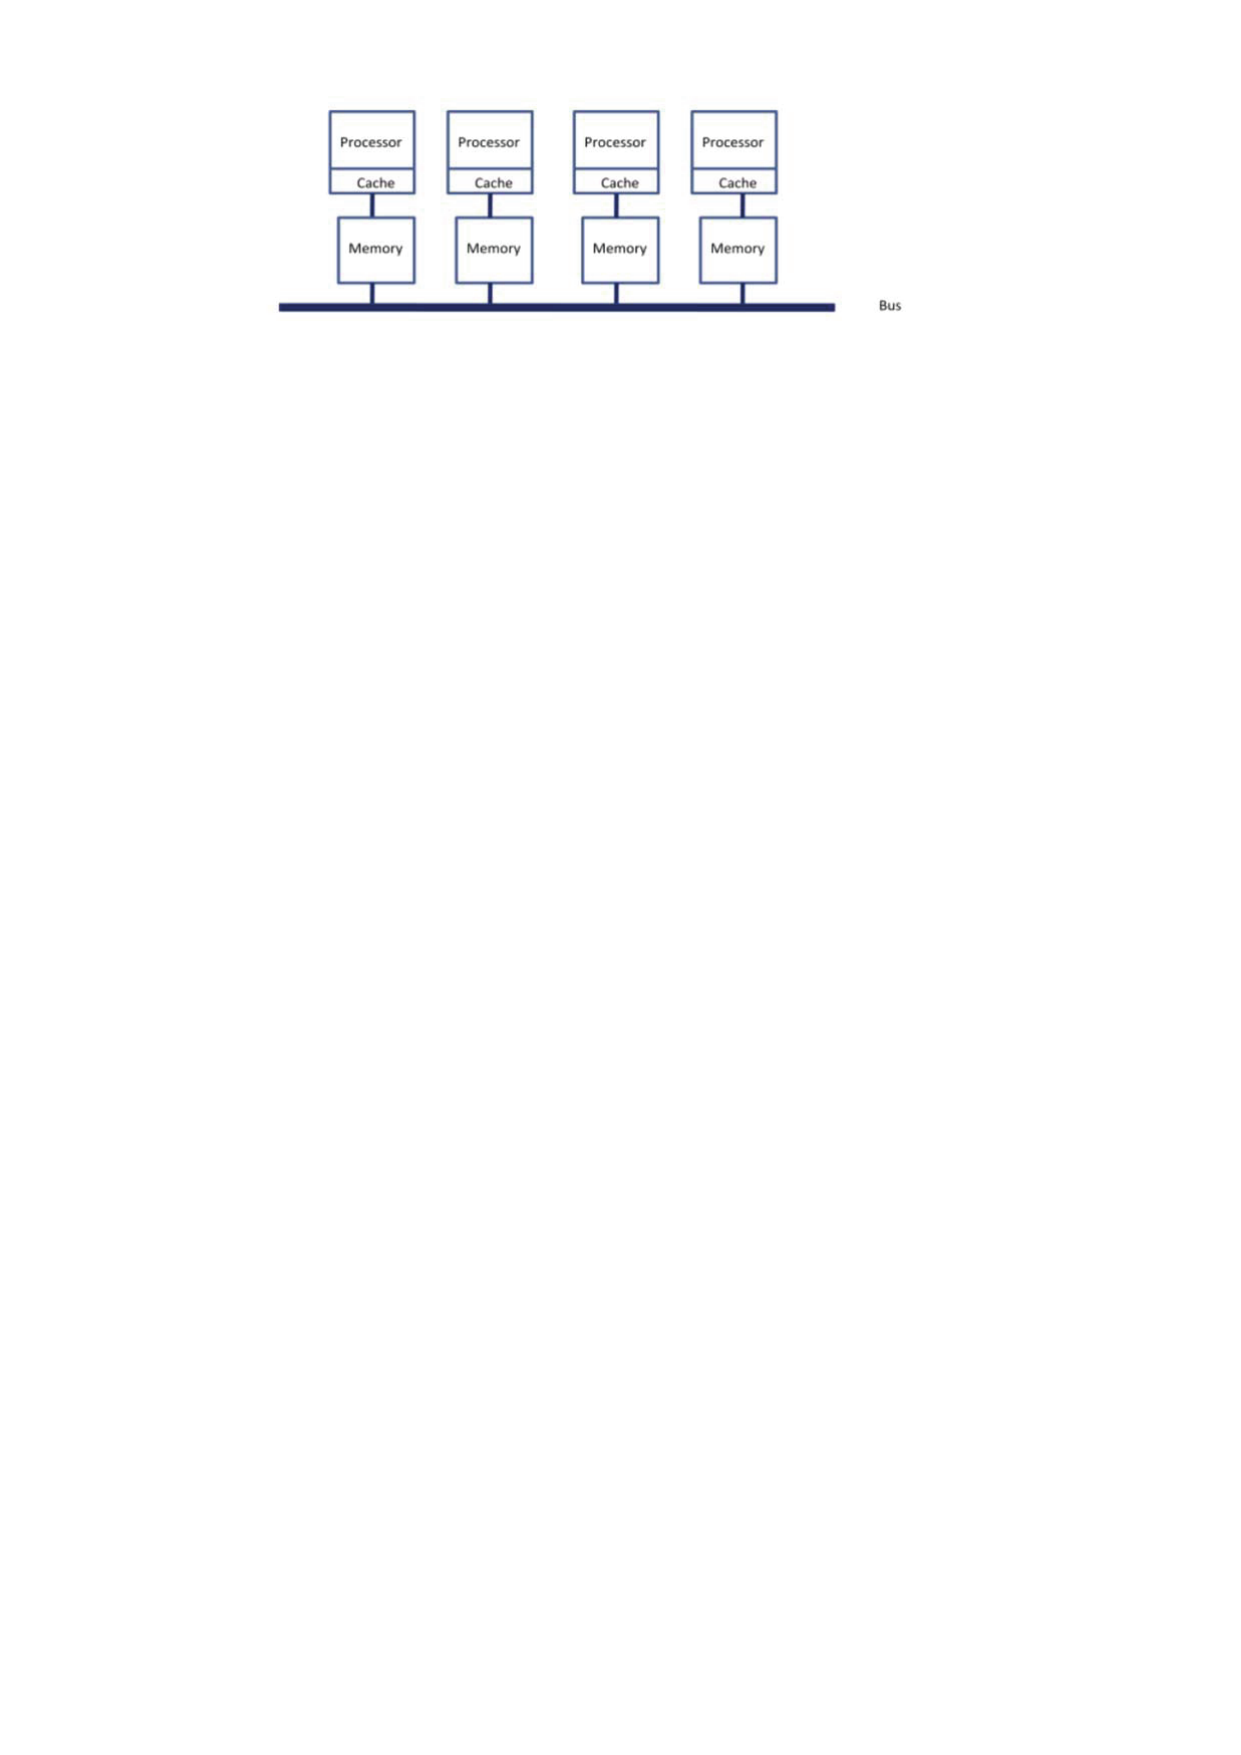
\includegraphics[scale=0.7890]{figures/fig-numa}

  \caption{Modern computer architecture using Non-Uniform momery
    access (NUMA).  }  \label{fig-numa}
\end{figure}


\textsc{Bpp4} can use multiple cores/threads.  The control variable
threads has the following syntax.
\begin{verbatim}
Threads = 8 19 1
\end{verbatim}
This means \textsc{bpp} will use 8 threads, starting from core/thread
19, with increment 1; in other words hardware threads 19-36 will be
used.  The software threads are pinned onto the hardware threads and
they not allowed to migrate.  We found that this helps with
performance.

Modern clusters based on microprocessors use a common shared-memory
configuration called NUMA (for non-uniform memory access).  The
cluster typically consists of two or four microprocessors
interconnected on a local bus to a shared memory on a single
motherboard.

You can use commands like \texttt{lscpu} to see the machine
architecture.  For example, on our server lscpu gives the following
output:

\begin{verbatim}
Architecture:          x86_64
CPU op-mode(s):        32-bit, 64-bit
Byte Order:            Little Endian
CPU(s):                144
On-line CPU(s) list:   0-143
Thread(s) per core:    2
Core(s) per socket:    18
Socket(s):             4
NUMA node(s):          4
...
NUMA node0 CPU(s):     0-17,72-89
NUMA node1 CPU(s):     18-35,90-107
NUMA node2 CPU(s):     36-53,108-125
NUMA node3 CPU(s):     54-71,126-143
\end{verbatim}
This means that hardware threads 1-18 are on CPU0, while threads 73-90
are the hyperthreads on CPU0.  The specification Threads = 8 19 1 thus
uses 8 threads on CPU1.  Our recommendation is that you do some tests
yourself using threads = 2 or 4 or 8, and use options that work well
for your servers.  Adjust the step lengths first.  Then use burnin=0
and a small nsample so that the running time is about 1-2 minutes.
Change threads and record running time.

Make sure all threads for the same \textsc{bpp} job are on the same
CPU.  Use lscpu to see the machine configuration and htop to examine
the load on the hardware threads.


\subsection{Checkpointing}

This option instructs \textsc{bpp} to create a checkpoint file (save
the progress) after a specified number of MCMC iterations.  The MCMC
loop in \textsc{bpp} consists of \texttt{N = burnin +
  sampfreq*nsample} iterations, numbered as $1,2,\cdots,N$.  There are
two formats, where X, Y are whole numbers:

\begin{verbatim}
checkpoint = X
checkpoint = X Y
\end{verbatim}
In the first format, a single checkpoint is created after X MCMC
iterations (including burnin).

In the second format, a checkpoint is created after X steps, and then
additional checkpoints are created every Y steps.  For example, if X =
10000 and Y = 10000, the first checkpoint is created at MCMC iteration
10000, and further checkpoints at iterations 20000, 30000, etc.

The checkpoint files are named OUTFILE.Z.chk, where OUTFILE is the
label specified for the outfile option, and Z is the number of the
checkpoint file, starting from 1 and incrementing with every new
checkpoint file.

To resume from a checkpoint file, use the resume switch, i.e.
\begin{verbatim}
bpp --resume checkpoint-file.chk
\end{verbatim}

\section{Marginal Likelihood Calculations}
The C program BFdriver generates control files and job subscription
scripts for running MCMC (using BPP or MCMCtree) to calculate the
marginal likelihood (or the Bayes factor), as described in
\citet{Rannala2017}.

The program takes a control file you provide (such as bpp.ctl) and
generates $K = 16$ control files with different beta values, which are
used to run bpp to sample from the different power posterior
distributions.  The program also generates job submission scripts and
submit the jobs using qsub.  All generated control files and output
files are in the same current directory.  The frogs dataset in the bpp
release \citep{Yang2015} is used as the example.

You need the following: a linux system with SUN grid engine managing
job submission (including commonds such as \texttt{qsub},
\texttt{qstat}, \texttt{qdel}, etc.), and a C compiler.  If you don't
have this job submission system, you can use BFdriver to generate the
control files and run the MCMC jobs from the command line.

\subsection{Compiling and running BFdriver}
\begin{verbatim}
cc -o BFdriver -O3 BFdriver.c tools.c -lm
BFdriver <controlfilename> <npoints> <scriptname.sh>
BFdriver A00.ctl 16 tmp.sh
\end{verbatim}

You may need to edit the following two lines inside BFdriver.c, and if
you do, remember to compile the program after editing.  Here bpp is
assumed to be on your search path.  You can use a full path for the
executable prorgam, such as \texttt{/home/gooduser/bin/bpp3.3}.  Also
the second line is for submitting the jobs using \texttt{qsub}.  Here
the limits are set to 4G of RAM and 360 hours of running time.  Check
those values if necessary (and recompile).
\begin{verbatim}
fprintf(fcommand, "     echo \"bpp %s.b$I.ctl > log.b$I.txt\" > %s\n", ctlf, scriptf);
fprintf(fcommand, "     qsub -S /bin/bash -l h_vmem=4G -l tmem=4G -l h_rt=360:0:0 -cwd %s\n", scriptf);
\end{verbatim}

\subsection{Running the program }

Create a folder inside \texttt{frogs/}, say \texttt{bf1}:
\begin{verbatim}
mkdir frogs/bf1
cd frogs/bf1
\end{verbatim}

Prepare a control file (A00.ctl, say) for the A00 analysis in the
folder.  Check that it works.  This should have a fixed species tree,
which is ((K, C), (L, H)).  Species delimitation and species tree
estimation should be turned off.  The control file specifies the
priors for theta, tau, and also specifies burnin, nsample, sampfreq
etc.  Run bpp to confirm that the control file works.  Then run
BDdriver as follows:

\begin{verbatim}
BFdriver A00.ctl 16 tree1.sh
\end{verbatim}

Here A00.ctl is the control file we have prepared.  $K = 16$ is the
number of points in the Gauss-Legendre qradrature algorithm for
numerical integration.  You can use 8 for testing, and 16 or 32 for
real calculation.  \texttt{tree1.sh} is the temporary script file for
job submission using \texttt{qsub}.  The BFdriver command does a few
things.  First it reads the control file specified (\texttt{A00.ctl})
and creates 16 control files with names like \texttt{A00.b01.ctl},
..., \texttt{A00.b16.ctl}.  Each of those control files has the same
content as \texttt{A00.ctl} except that one extra line is inserted at
the beginning, like the following
\begin{verbatim}
BayesFactorBeta = 0.122298 *  w=0.124629.ctl
\end{verbatim}
This specifies the beta value when the control file is used to run
\textsc{bpp}.

Second \texttt{BFdriver} creates a file named
\texttt{betaweights.txt}, which lists the beta values and
Gauss-Legendre weights.  I have copied those values into an excel file
in \texttt{frogs/BFdriver.frogs.xls}.

Third \texttt{BFdriver} creates a file named commands, which has the
bash shell scripts for submitting the 16 jobs using \texttt{qsub}.
You use the following to submit the jobs.
\begin{verbatim}
source commands
\end{verbatim}

You can look at the content of \texttt{tree1.sh} to see the script for
the last job:
\begin{verbatim}
more tree1.sh
\end{verbatim}
which should have the content like the following:
\begin{verbatim}
bpp --cfile bpp.b16.ctl > log.b16.txt
\end{verbatim}

You can use \texttt{qstat} to check the status of the 16 jobs you have
submitted.  When the jobs are running, they generate output files in
the current folder, such as \texttt{mcmc.b01.txt},
\texttt{out.b01.txt}, and \texttt{log.b01.txt} (which logs the screen
output).  After all jobs are finished, you can use grep to extract the
line with \texttt{BFbeta} from screen log (this command is at the
bottom of the file commands).
\begin{verbatim}
grep BFbeta log.b*.txt
\end{verbatim}
Then copy the ElnfX values into the excel file, and estimate the
logarithm of the marginal likelihood by summing (\texttt{weights *
  ElnfX / 2}) over the 16 points. This gives the log marginal
likelihood to be $-3185.93$.

\subsection{Exercise and results}

Duplicate the calculation for the alternative species tree (tree2) in
the folder /bf2.  Change the species tree topology to (((L, H), C),
K), and use tree2.sh as the temporary job script file.  Everything
else should be the same as described above.

My runs gave the log marginal likelihood for tree 2 to be $-3186.14$.
The ratio of the posterior probabilities for the two trees is then
estimated to be
$P_1/P_2 = \exp\{-3185.93 - (-3186.14)\} = exp\{0.21\} = 1.24$.  With
\textsc{bpp}4.0 and the inverse-gamma priors on $\theta$ and $\tau$s,
the MCMC runs (A01) gave the posterior probabilities for trees 1 and 2
as 0.167 and 0.137, with the ratio 1.22.  The MCMC runs and the
marginal likelihood calculations seem to agree with each other.  (Note
that with \textsc{bpp3} and the gamma priors on $\theta$ and $\tau$s,
the posteriors are 0.16 and 0.13 with the ratio 1.2
\citep[][fig.~4]{Yang2015}.

\subsection{Common errors and problems}

Check the bpp control file by running bpp at the command line before
submitting the jobs.  Make sure that the bpp program is on your path
or use a full path.  You may have to edit the source file
\texttt{BFdriver.c} and recompile.


\chapter{Simulation Using BPP}

The simulation option of \textsc{bpp4} is the MCCOAL program in
version 3.4 and earlier.  This can be used to simulate gene trees and
sequence alignments at multiple loci under the MSC \citep{Rannala2003}
and MSci \citep{Flouri2020a} models.  While the inference program
\textsc{bpp} implements the JC model only, the simulation program
allows GTR+G (and its special cases) and allows among-loci
heterogeneity in the process of sequence evolution.  The different
loci can have different exchangeability parameters
($a, b, c, d, e, f$) and base compositions in the GTR model, different
overall evolutionary rates, different extent of among-site rate
variation (reflected in the alpha parameter for the gamma model), and
different among-branch rate drifts (violation of the clock).  See
\citet{Shi2018} for examples of such simulations.  The simulation
option also includes a continuous migration model, with a
user-specified migration rate matrix between species/populations.

Look at the \texttt{README.txt} file for compiling the program.  To
run the program, type one of the following.  The default control file
name is \texttt{MCcoal.ctl}.  Always look at the screen output to
confirm that the program reads the control file correctly.
\begin{verbatim}
bpp --simulate MCcoal.ctl
bpp --simulate MCcoalMigration.ctl
\end{verbatim}


\subsection{B1 Control-file options for simulating without migration}

Here is a sample control file.
\begin{verbatim}
seed = 12345
seqfile = MySeq.txt 0 * comment out this line if you don't want seqs
treefile = MyTree.tre  * comment out this line if you don't want trees
Imapfile = MyImap.txt
*   concatfile = concatenatedfile.txt  * concatenated alignment
modelparafile = modelparas.txt   * comment out this line if you don't want seqs

species&tree = 4  A  B  C  D
3  2  1  1
((A #0.01, B #0.01) :0.01 #.01, (C, D) :0.011 #0.01) : 0.012 #0.01;
phase =    1  1  1  0   * 0: do not phase (fully phased seqs), 1: diploid unphased seqs

loci&length = 100 1000 * number of loci & number of sites at each locus
*    locusrate = 0 (default: same rate for all loci)
*    locusrate = mu_bar a_mui prior
*        clock = 1 (default: strict clock)
*        clock = 2 v_bar a_vi prior dist  (independent-rates)
*        clock = 3 v_bar a_vi prior dist  (correlated-rates)

model = 7       * model: 0:JC69, 7:REV (GTR)
Qrates = 0  10 5 5 5 5 10     * 1: fixed; 0: dirichlet, for TC TA TG CA CG AG
basefreqs = 0  10  10  10  10   * 0: random, Dirichlet(aT,aC,aA,aG), for base frequencies
alpha_siterate = 0  100  20  5  * G(a, b) for alpha for sites & K for discrete gamma
\end{verbatim}

\texttt{seed} Use $-1$ to simulate different datasets every time the
program is run.  If you use a positive integer the data will stay
exactly the same, which is a bad idea.

\texttt{seqfile, treefile, Imapfile, concatfile, modelparafile.}
These are names of files to be generated.  If you want to simulate
gene trees and not sequence files, you can comment out the line for
the seqfile.  concatfile will have the sequence alignment concatenated
across loci.  The sequence files can become very large.  modelparafile
records the parameter values for the GTR model, as well as the locus
rate and the rates for nodes on the species tree.  There is one line
of output per locus.

By default MCcoal prints out the sequence alignment at each locus, but
if you use file format 1 (\texttt{seqfile = MySeq.txt 1}), the program
will print out site pattern counts instead. The file may then be
smaller.  This format is readable by \textsc{bpp} and \textsc{3s}, but
not by other programs.

\texttt{phase.}  This variable is used in the same way as in the
inference (data analysis) mode. Each species is assigned a
switch/flag, with 0 meaning fully phased (haplotype) sequences and 1
for unphased diploid sequences.  With the specifications in the
example (sampling configuration 3 2 1 1 and phase = 1 1 1 0), the
program will simulate 6, 4, 2, 1 sequences for A, B, C, D,
respectively, and then combine every two sequences from A, B, C into
one single diploid sequence with heterozygote sites represented using
ambiguity characters (YRMKSW).  If you use the same random number
seed, the diploid data generated using the sampling configuration (3 2
1 1) with phase = 1 1 1 0 should match the fully resolved sequences
generated using the sampling configuration (6 4 2 1) with phase = 0 0
0 0.  The program also prints out the fully resolved sequences in a
file with the suffix \texttt{\_full} (or \texttt{MySeq\_full.txt} in
the example).

\texttt{species\&tree.}  This block specifies the number and names of
species, the species tree, and the parameters under the multispecies
coalescent model, including the species divergence times ($\tau$s) and
population size parameters ($\theta = 4N\mu$).  For the example above,
100 loci, each of 1000 sites, will be simulated, on the species tree
((A, B), (C, D)), with 3, 2, 1, 1 sequences for A, B, C, D, so that
there are 7 sequences at each locus.  The divergence time parameters
($\tau$s) are after `:' in the tree, while the population size
parameters ($\theta$s) are after `\#'.  Thus we have 0.01 for all
$\theta$s, and $\tau_{ABCD} = 0.012$, $\tau_{AB} = 0.01$, and
$\tau_{CD} = 0.011$.  We need $\theta_A$ and $\theta_B$ because 2 or
more sequences are sampled from species A and B.  Parameters
$\theta_C$ and $\theta_D$ are unnecessary in this case as only one
sequence is sampled from C and D: if you specify them, they will be
ignored by the program.  Note that both $\theta$s and $\tau$s are
measured by the expected number of mutations per site, so that
$\theta = 0.01$ means that two sequences sampled from the population
are 1\% different.  For reference, the estimate for the human species
is $\theta_H = 0.0006$.

\texttt{model.} This can take two possible values: 0 for JC69 and 7
for GTR. The next few lines are relevant for the GTR model.

\texttt{Qrates} specifies the exchangeability parameters in the GTR
model ($a, b, c, d, e, f$ for TC, TA, TG, CA, CG, and AG, in
\citealt{Yang1994a}). There are two options, either to have those
rates fixed for all loci or to have them sampled at random.  The first
has the following format (note that the first 0-1 number is a switch):
\begin{verbatim}
Qrates = 1  2 1 1 1 1 2   *  1: fixed; for TC TA TG CA CG AG
\end{verbatim}

The input is one integer value (0 or 1) which acts as a switch
followed by six real numbers. The line above fixes the rates at
$a = 2, b = c = d = e = 1$ and $f = 2$, so that the transition rate is
twice as high as the transversion rate, and the model corresponds to
K80 or HKY.  Note that only the relative rates matter, because the
rate matrix ($Q$) is scaled so that the average rate (over the base
frequencies) is 1 and branch lengths are measured in the expected
number of mutations/substitutions per site.  Nevertheless the program
expects six rate parameters in the input here.
\begin{verbatim}
Qrates = 0  10 5 5 5 5 10   *  0: dirichlet, for TC TA TG CA CG AG
\end{verbatim}
The second option, above, is to sample $a, b, c, d, e$ from the
Dirichlet distribution for every locus.  The above specifies Dir(10,
5, 5, 5, 5, 10), with parameters
$\alpha_a = 10, \alpha_b = \alpha_c = \alpha_d = \alpha_e = 10$, and
$\alpha_f = 10$.  The rates generated from the Dirichlet sum to 1, and
they are rescaled.  Note that larger values for those parameters mean
less variance, while the mean for $a$, say, is given by
$\alpha_a/\alpha$ with
$\alpha = \alpha_a + \alpha_b + \alpha_c + \alpha_d + \alpha_e +
\alpha_f$.  The specification here gives on average a
transition/transversion rate ratio of 2 (if the base frequencies are
fixed at $\frac{1}{4}$ each), but it varies among loci.

\texttt{basefreqs.} The base frequency parameters
($\pi_T, \pi_C, \pi_A, \pi_G$) can also be fixed or sampled from the
Dirichlet distribution, like the \texttt{Qrates}.  The two options are
as follows.
\begin{verbatim}
basefreqs = 1 0.15 0.35 0.15 0.35  * 1: fixed; Base frequencies are for TCAG.
basefreqs = 0  10  10 10  10       * 0: random, Dirichlet(aT, aC, aA, aG), for base frequencies
\end{verbatim}

\texttt{alpha\_siterate.}  The gamma shape parameter ($\alpha$) for
rate variation among sites of the same locus can be fixed or sampled
from a gamma distribution.  The possible options are as follows.  When
alpha is fixed, the same value is used for all loci.  Otherwise
different $\alpha$s are used for different loci.  Note that given
alpha, the rates for sites at the same locus have a
G(($\alpha, \alpha$) distribution with mean 1 \citep{Yang1993,
  Yang1994b}.  The fourth option below will allow the program to sample
$\alpha$ from $G(100, 20)$, with mean 5, for each locus and then use
$G(\alpha, \alpha)$ to describe the among-site rate variation for the
locus.
\begin{verbatim}
alpha_siterate = 1 0            * 1: alpha fixed at 0(inf), one rate for all sites at the locus
alpha_siterate = 1  5.6 0       * 1: alpha fixed at 5.6, K = 0(inf) for continuous gamma
alpha_siterate = 1  5.6 5       * 1: alpha fixed at 5.6, K = 5 categories for discrete gamma
alpha_siterate = 0  100  20  5  * 0: alpha sampled from G(100, 20), with mean 5, K = 5 for discrete gamma
\end{verbatim}

\texttt{locusrate.}  The variables \texttt{locusrate} and
\texttt{clock} are used to specify relaxed-clock models, with rate
variation among branches and among loci.  These are the same models as
implemented in the inference program.  Please see notes in section ??
for details.

\texttt{locusrate} specifies variable rates for different loci.  The
default is 0, meaning that all loci have the same rate.  To specify
variable rates for loci, use the following format.
\begin{verbatim}
locusrate = 0 (default)
locusrate = mu_bar a_mui prior
locusrate = mu_bar a_mui
locusrate = 1.0 5.0 dir
\end{verbatim}
Here \texttt{mu\_bar} is the mean rate across loci.

If \texttt{prior = dir} (gamma-Dirichlet), the total rate ($L\bar\mu$)
is partitioned to generate the locus-rates ($\mu_i$) according to the
Dirichlet distribution with concentration parameter $\alpha$
(\texttt{a\_mui}).  Large $\alpha$ (10 or 100, say) means that the
rates are similar among loci, while small values (1 or 0.5, say) mean
that rates are highly variable among loci. If \texttt{prior = iid}
(conditional i.i.d.), the locus rates ($\mu_i$) are i.i.d. given the
mean rate ($\bar\mu$):
\begin{verbatim}
mu_i ~ Gamma(a_mui, a_mui/mubar)
\end{verbatim}

\texttt{clock.}  This is used to specify strict-clock or relaxed-clock
models.  The default is \texttt{clock = 1} for strict clock, while
\texttt{clock = 2} is the independents-rates model, and \texttt{clock
  = 3} is the correlated-rates model (which is implemented for the MSC
model with no introgression and is unavailable for the MSci model).
\begin{verbatim}
clock = 1 (default: strict clock)
clock = 2 v_bar a_vi prior dist  * independent-rates model
clock = 2 0.1 10 dir G    * gamma-dirichlet for loci & gamma for branches
clock = 2 0.1 10 iid LN   * iid for loci & log-normal for branches
clock = 3 v_bar a_vi prior dist  * correlated-rates model
clock = 3 0.1 10 iid G    * iid for loci & gamma for branches
clock = 3 0.1 10 iid LN   * iid for loci & log-normal for branches
\end{verbatim}
The specification (\texttt{clock = 2 0.1 10 dir G}) means the
following.  First the average variance parameter is = 0.1.  Then the
total $L\bar\mu$ is partitioned into $\mu_i$ (for
$i = 1, 2, \cdots, L$) according to the Dirichlet distribution with
concentration parameter $\alpha = 10$ (\texttt{a\_vi}).

In contrast, the specification (\texttt{clock = 2 0.1 10 iid LN})
means that the variance parameter for locus $\nu_i$ is generated as
$\nu_i|\bar\nu \sim G(\alpha, \alpha/\bar\nu)$ with shape parameter
$\alpha = 10$ (\texttt{a\_vi}) and mean $\bar\nu = 0.1$.

In both prior models (\texttt{prior=dir} and \texttt{iid}), $\alpha$
(\texttt{a\_vi}) is inversely related to the variance in $\mu_i$ among
loci: use small values of $\alpha$ (2, 1, or 0.5) if the clock nearly
holds at some loci but is seriously violated at others, and large
values (such as 10 or 100) if the clock is violated in the same extent
at different loci.

\texttt{clock = 2.} Given the locus rate $\mu_i$ (specified using the
\texttt{locusrate} variable) and the variance parameter $\nu_i$
(specified using the \texttt{clock} variable) for locus $i$, the rates
for species-tree branches are specified as follows.  If \texttt{dist =
  G} (for gamma), the rate for branch $j$ at locus $i$ has the
following gamma distribution with mean $\mu_i$ and variance $\nu_i$
\begin{equation*}
  r_{ij} | \mu_i, \nu_i \sim G(\mu_i^2/\nu_i, \mu_i/\nu_i).
\end{equation*}

If \texttt{dist = LN} (for log-normal), the rate has the log-normal
distribution
\begin{equation*}
  r_{ij} | \mu_i, \nu_i \sim LN(\mu_i, \nu_i).
\end{equation*}

\texttt{clock = 3.}  The correlated-rates model is specified
similarly, and for the MSC model only.  Given the locus rate $\mu_i$
(specified using the \texttt{locusrate} variable) and the variance
parameter $\nu_i$ (specified using the \texttt{clock} variable) for
locus $i$, the rates for species-tree branches are specified
recursively, starting from the root towards the tips.

If \texttt{dist = G} (for gamma), the rate for branch $j$ at locus $i$
has the following gamma distribution with shape parameter
$\alpha = \mu_i^2/\nu_i$ and with the mean to be the rate for the
parental branch of $j$ or $r_{i,p(j)}$:
\begin{equation*}
  r_{ij} | \mu_i, \nu_i, r_{i,p(j)} \sim G(\frac{\mu_i^2}{\nu_i}, \frac{\mu_i^2}{\nu_i r_{i,p(j)}}).
\end{equation*}
If \texttt{dist = LN} (for log-normal), the rate for branch $j$ at
locus $i$ has the log-normal distribution with the mean to be the
parental rate and variance parameter $\nu_i$:
\begin{equation*}
  r_{ij} | \nu_i, r_{i,p(j)} \sim LN(r_{i,p(j)}, \nu_i).
\end{equation*}

After the rates for branches (populations) on the species tree are
generated for the locus, they are used to calculate the gene-tree
branch lengths.  Gene-tree branches residing in the same
species/populations have the same rate (the rate of that species at
the locus), while those residing in different species may have
different rates.  A branch on a gene tree may have segments residing
in different species/populations, and the length of the branch
(measured by the expected number of mutations/substitutions per site)
is calculated by adding up those segments.


\subsection{B2 Simulating with migration (under the IM model)}

\begin{verbatim}
migration = 7   * number of pops (order fixed by program)

A     B     C     D    ABCD    AB   CD
A      0     1.1   1.2   1.3    0     0    -1
B      0.1   0     1.4   1.5    0     0    -1
C      0.2   0.4   0     1.6    0     1.7   0
D      0.3   0.5   0.6   0      0     1.8   0
ABCD   0     0     0     0      0     0     0
AB     0     0     0.7   0.8    0     0     1.9
CD    -1    -1     0     0      0     0.9   0
\end{verbatim}

The control file for simulating migration as well as coalescence
includes a block as above (see the file \texttt{MCcoalMigration.ctl}).
The line \texttt{migration = 7}, where 7 is the number of populations
on the species tree, tells the program to simulate migrations.  This
number is fixed by the species tree and is used here for error
checking.  This is then followed by a migration matrix, of size
$7\times 7$.  The names of the populations are read and ignored by the
program, and the order of the populations is fixed.  You should run
the program without the migration matrix first and then use the screen
output to use the correct order of populations to specify the
migration matrix.

In the migration matrix, values 0 and $-1$ mean that migration is
either impossible (for example, if the two populations did not live at
the same time) or not allowed (if the two populations were
contemporary but no migration between them is assumed to occur).  Use
0 for both cases here.  Positive values are scaled migration rates,
with the element on the $i$th row $j$th column to be
$M_{ij} = N_j m_{ij}$, where $m_{ij}$ is the migration rate per
generation in population $j$ from population $i$, or the proportion of
individuals in population $j$ that are immigrants from population $i$,
and where $\mu$ is the mutation rate per site per generation. In the
example above, $M_{A\to B} = 1.1$, which means that on average 1.1
individuals are immigrants from population $A$ to population $B$.

Note that the $\theta$ parameter for a modern species has to be
specified in the tree file even if only one sequence is sampled from
that species but migrations into that species are allowed by the
migration matrix.


\section{Features New To BPP 4.0}

\begin{itemize}
\item i.  Multiple threads
\item ii.  Introgression model (MSci)
\item iii. Local-clock and locus-rates models (clock and locusrate)
\item iv.  Topological constraints (constraint and outgroup)
\end{itemize}



\newpage
\bibliographystyle{natbib} \bibliography{bpp-4-manual.bib}



\end{document}
